\clearpage
\section{Event selection}
\label{sec:event-selection}

As discussed in Section~\ref{sec:search-strategy}, three event categories are used in this analysis: the dimuon category and an exclusive track category for each lepton flavor (muon and electron). The preselection is summarized in Section~\ref{sec:preselection}, followed by the selection that defines each category in Section~\ref{sec:category-selection}. Finally, the multivariate selection for each category is discussed in Section~\ref{sec:event-bdt}.

\subsection{Preselection}
\label{sec:preselection}

In Section~\ref{tab:base-selection}, the preselection criteria that apply to all categories was defined. This section reiterates the reasons for this selection as well as describes other event-level selection.

\begin{itemize}

\item $\mht\geq220\GeV$ and $\MET \geq 140\GeV$ cuts are intended to boost sensitivity by rejecting \gls{sm} background and to operate in the acceptance regime of the MET trigger, as described in Section~\ref{sec:trigger}. These cuts are especially efficient in rejecting \gls{qcd} background, which does not produce real \MET. Any \MET apparent in \gls{qcd} is due to jet energy miss-measurements. The harder cut on \mht is made instead of \MET because \mht sums jets with $\pt>30\GeV$ and is blind to objects with $\pt<30\GeV$. Background estimation relies on jets with \pt in the range of $[15,30]\GeV$, so \mht avoids introducing bias in the data-driven background estimation methods.

\item $\njets \left( \pt \geq 30\GeV\, \mathrm{and}\, \abs{\eta} < 2.4 \right) \geq 1$. At least one jet is required in the event because such an \gls{isr} jet gives a boost to the produced neutralino, thus increasing the missing transverse energy and the sensitivity of the analysis.

\item $\nbjets \left( \pt \geq 30\GeV\, \mathrm{and}\, \abs{\eta} < 2.4 \right) = 0$. Any event with \PQb-tagged jet is vetoed since our signal does not contain real \PQb-tagged jets. This veto is efficient in rejecting background from \ttbar, in which the \PQb quarks arise from a \PQt quark decay.

\item $\mindphimhtjets$  $ > 0.4$. Requiring an \gls{isr} jet in the event leads to the expectation that the $\mht$ should point in the opposite direction of the jet or at an angle close to $\pi$. Events with multiple jets in the \gls{sm} background, such as those arising from \gls{qcd}, will not exhibit such a feature. Therefore, this cut reduces the \gls{qcd} background.

\item veto events with isolated loose-ID lepton having $\pt\geq 30\GeV$. Lepton can be either muon or electron.

\item $0.4<\mll<12 \GeV$. The signal resides in an invariant mass window with an edge at the mass difference between \neutt and \neuto. This is a relatively loose cut that is expected to be further tightened by the boosted decision tree.

\end{itemize}

The object level selection was described in detail in Section~\ref{sec:object-selection}. For the sake of completeness it is reiterated. The electrons in the analysis require are required to pass the following selection (also described in Section~\ref{sec:object-selection-electrons}):

\begin{itemize}

\item $5 \leq \pt \leq 15\GeV$;
\item $\abs{\eta} < 2.5$;
\item pass jet isolation;
\item loose ID.

\end{itemize}

The muons in the analysis are required to pass the following selection (see also Section~\ref{sec:muon-selection}):

\begin{itemize}

\item $2 \leq \pt \leq 15\GeV$;
\item $\abs{\eta} < 2.4$;
\item pass jet isolation;
\item medium ID.

\end{itemize}

\subsection{Category selection}
\label{sec:category-selection}

The analysis includes three main categories: the dilepton category and an exclusive track category for each lepton flavor. The dilepton category requires two fully-identified leptons, both of which are muons. In contrast, the exclusive track category includes a single lepton and a track that has not been identified as a lepton. Both electrons and muons are accepted as the single lepton in the exclusive track category. The selection criteria for the dilepton category are described in Section~\ref{sec:dilepton-selection}, while those for the exclusive track category are detailed in Section~\ref{sec:exclusive-track-selection}.

\subsubsection{Dilepton selection}
\label{sec:dilepton-selection}

In the dilepton category, two reconstructed and identified muons are required. Events in the di-lepton category must satisfy the preselection and the baseline selection, as well as the following criteria:

\begin{itemize}

\item $N_\mu = 2$ - opposite-charge satisfying the analysis muon selection;
\item $\pt(\mu_2)\leq 3.5\GeV$ or $\DR(\mu_1,\mu_2) < 0.3$. This requirement ensures the analysis is orthogonal, that is, non-overlapping in terms of event content, with the previously published soft lepton analysis~\cite{sos};
\item Event BDT score $\mathrm{BDT} > 0$. This is the main method of selecting signal events while rejecting the \gls{sm} background. Details are given in Section~\ref{sec:event-bdt};
\item $\DR(\mu_{1,2},j_1) > 0.4$, where $j_1$ is the leading jet. The leptons should not be inside the \gls{isr} jet;
\item \PGo, $\PGr^0$ and \JPsi invariant mass vetoes. $\mll \notin [0.75,0.81]\GeV,\,\mll \notin [3,3.2]\GeV$.
\end{itemize}

\subsubsection{Exclusive track selection}
\label{sec:exclusive-track-selection}

The exclusive track category requires one reconstructed and identified lepton, which can be either an electron or a muon, and an exclusive track, meaning a track that is not identified as a lepton. The track with the highest track \gls{bdt} score, as described in Section~\ref{sec:track-bdt}, is picked as the signal lepton candidate. Events in this category must satisfy the preselection and the baseline selection, as well as the following criteria:

\begin{itemize}

\item $N_\ell = 1$ lepton passing the analysis muon or electron selection;
\item maximum track picking BDT score $ > 0$, as discussed in~\ref{sec:track-bdt};
\item event level BDT score $ > 0$. This is the main method of selecting signal events while rejecting the \gls{sm} background. , as discussed in Section~\ref{sec:event-bdt};
\item $\DR(\ell,j_1) > 0.4$, where $j_1$ is the highest-pT jet. The lepton should not be inside the \gls{isr} jet.
\end{itemize}

\subsection{Binary event classifier}
\label{sec:event-bdt}

This analysis employs a multivariate classifier to select signal events while optimally rejecting SM background events. The classifier algorithm is a \gls{bdt}, and its output score is used to define \glsreset{sr}\glspl{sr} as well as \glsreset{sr}\glspl{cr}. For the dimuon category, one \gls{bdt} is trained, while for the exclusive track category, a \gls{bdt} is trained for each lepton flavor and for the two phases of the tracker detector (Phase 0 and Phase 1), resulting in a total of five \glspl{bdt}.

All \glspl{bdt} are based on the same architecture, making use of 120 trees with a maximum depth of 3. The \gls{bdt} training is performed with AdaBoost and GiniIndex separation. The BDTs are trained and evaluated using the TMVA package~\cite{tmva}. 

For training, signal events are taken from the dedicated samples used to train the track-picking BDT for the exclusive track category, listed in Section~\ref{sec:signal-simulation} for the signal, and SM samples listed in Section~\ref{sec:sm-mc} for the background. For the exclusive track category, MC from 2016 and 2017 are used to represent Phase 0 and Phase 1 of the tracker, respectively. For the dimuon category, only 2017 MC is used to represent both phases, with an added systematic uncertainty resulting from this choice.

For the signal the same broad range of higgsino parameter $\mu$ (\PSGcpmDo) is used as was considered for the track-picking BDT training sample, but only the range of \dm targeted by the analysis. For Phase 0, $\dmo$ is selected in the range of [0.3, 4.3]\GeV and $\mu$ is selected in the range [100,130]\GeV. For Phase 1, $\dmpm$ is selected in the range of [0.3-4.6]\GeV and $\mu$ is selected in the range of [100-500]\GeV. The preselection and baseline selection is applied to the events included in the training, as well as a subset of the selection criteria listed in Section~\ref{sec:dilepton-selection} and Section~\ref{sec:exclusive-track-selection} as follows:

\begin{itemize}

\item $N_\mu = 2 (1)$ opposite-charge passing the muons selection for the dimuon category (for the exlusive track category);

\item $\DR(\ell),\text{leading jet}) > 0.4$;

\item track picking BDT score $ > 0$ for the exclusive track category.

\end{itemize}

The training was conducted without using \gls{mc} weights to avoid possible overtraining issues. This choice does not compromise the performance of the BDT because the kinematics of low-\pt leptons are similar across most \gls{sm} background production processes. When examining the distributions of input variables in the following sections, this fact must be taken into account. The distributions are plotted without \gls{mc} weights and with signal events taken from a pool of different parameter values as described above. Therefore, the ROC curves cannot be understood as a simple signal efficiency versus background rejection. Each \gls{bdt} output working point results in a different signal efficiency depending on the signal parameter values. As will be seen later, one does not use a single value of \gls{bdt} with a simple cut and count. Instead, the \glspl{sr} are binned according to \gls{bdt} output values. Therefore, the ROC curve is plotted with a default cut of 0.0 for the sake of completeness. To fully estimate the power of the training, one needs to consider the significance when each signal point has been properly weighted together with the background processes from the \gls{sm}.

\subsubsection{Dimuon category}

The training samples for the dimuon category contain 4350 signal events and 21842 background events. The \gls{bdt} evaluated in statistically independent samples of the same size in order to identify any overtraining. The distributions of the testing samples superimposed on the training samples, as well as the ROC curve, are shown in Figure~\ref{fig:event-bdt-dimuon-output}. No significant overtraining is observed. The BDT takes 18 variables as input, listed in Table~\ref{tab:dimuon-bdt-variables} in decreasing order of importance ranking.

\begin{figure}[!htb]
\centering
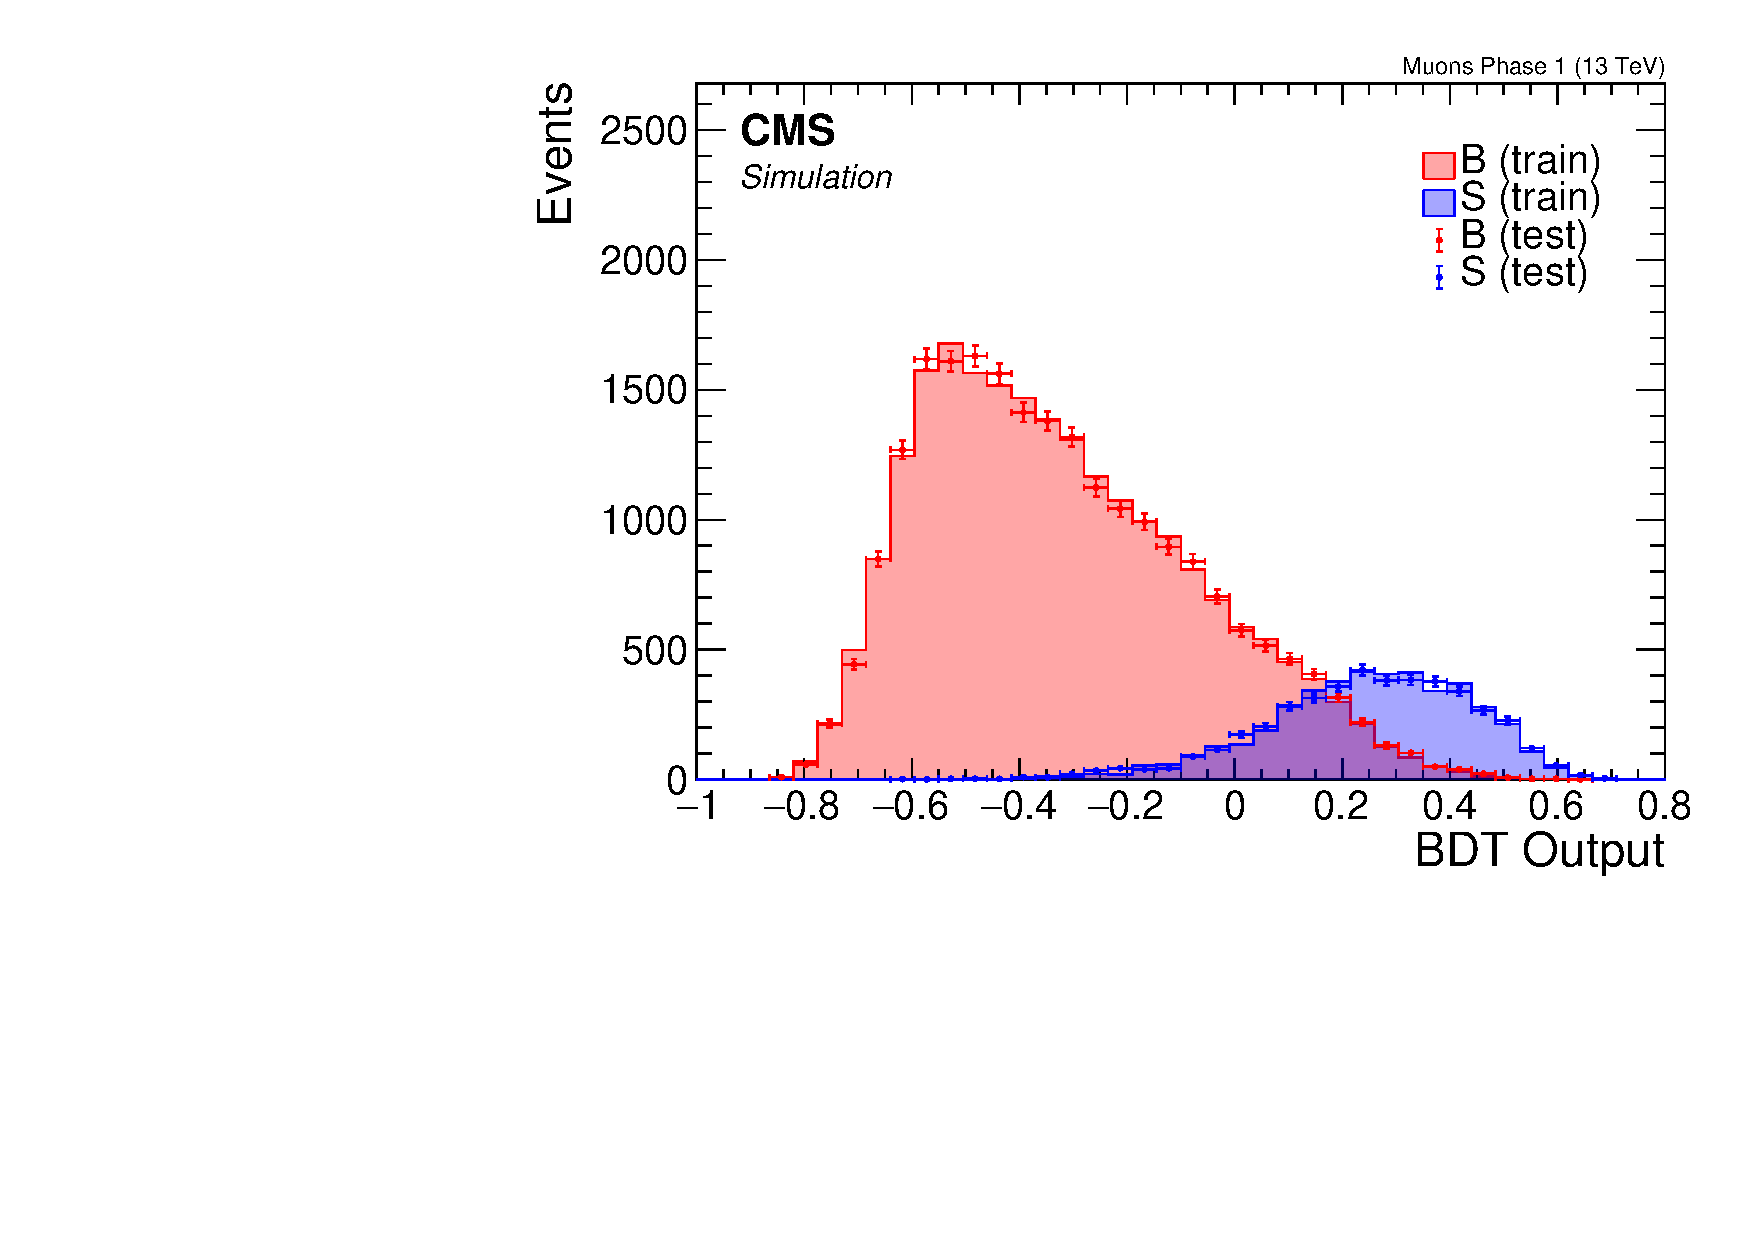
\includegraphics[width=0.48\linewidth]{plots/dimuon_bdt/overtraining_Event_Dilepton_Muons_Phase_1.pdf} \,
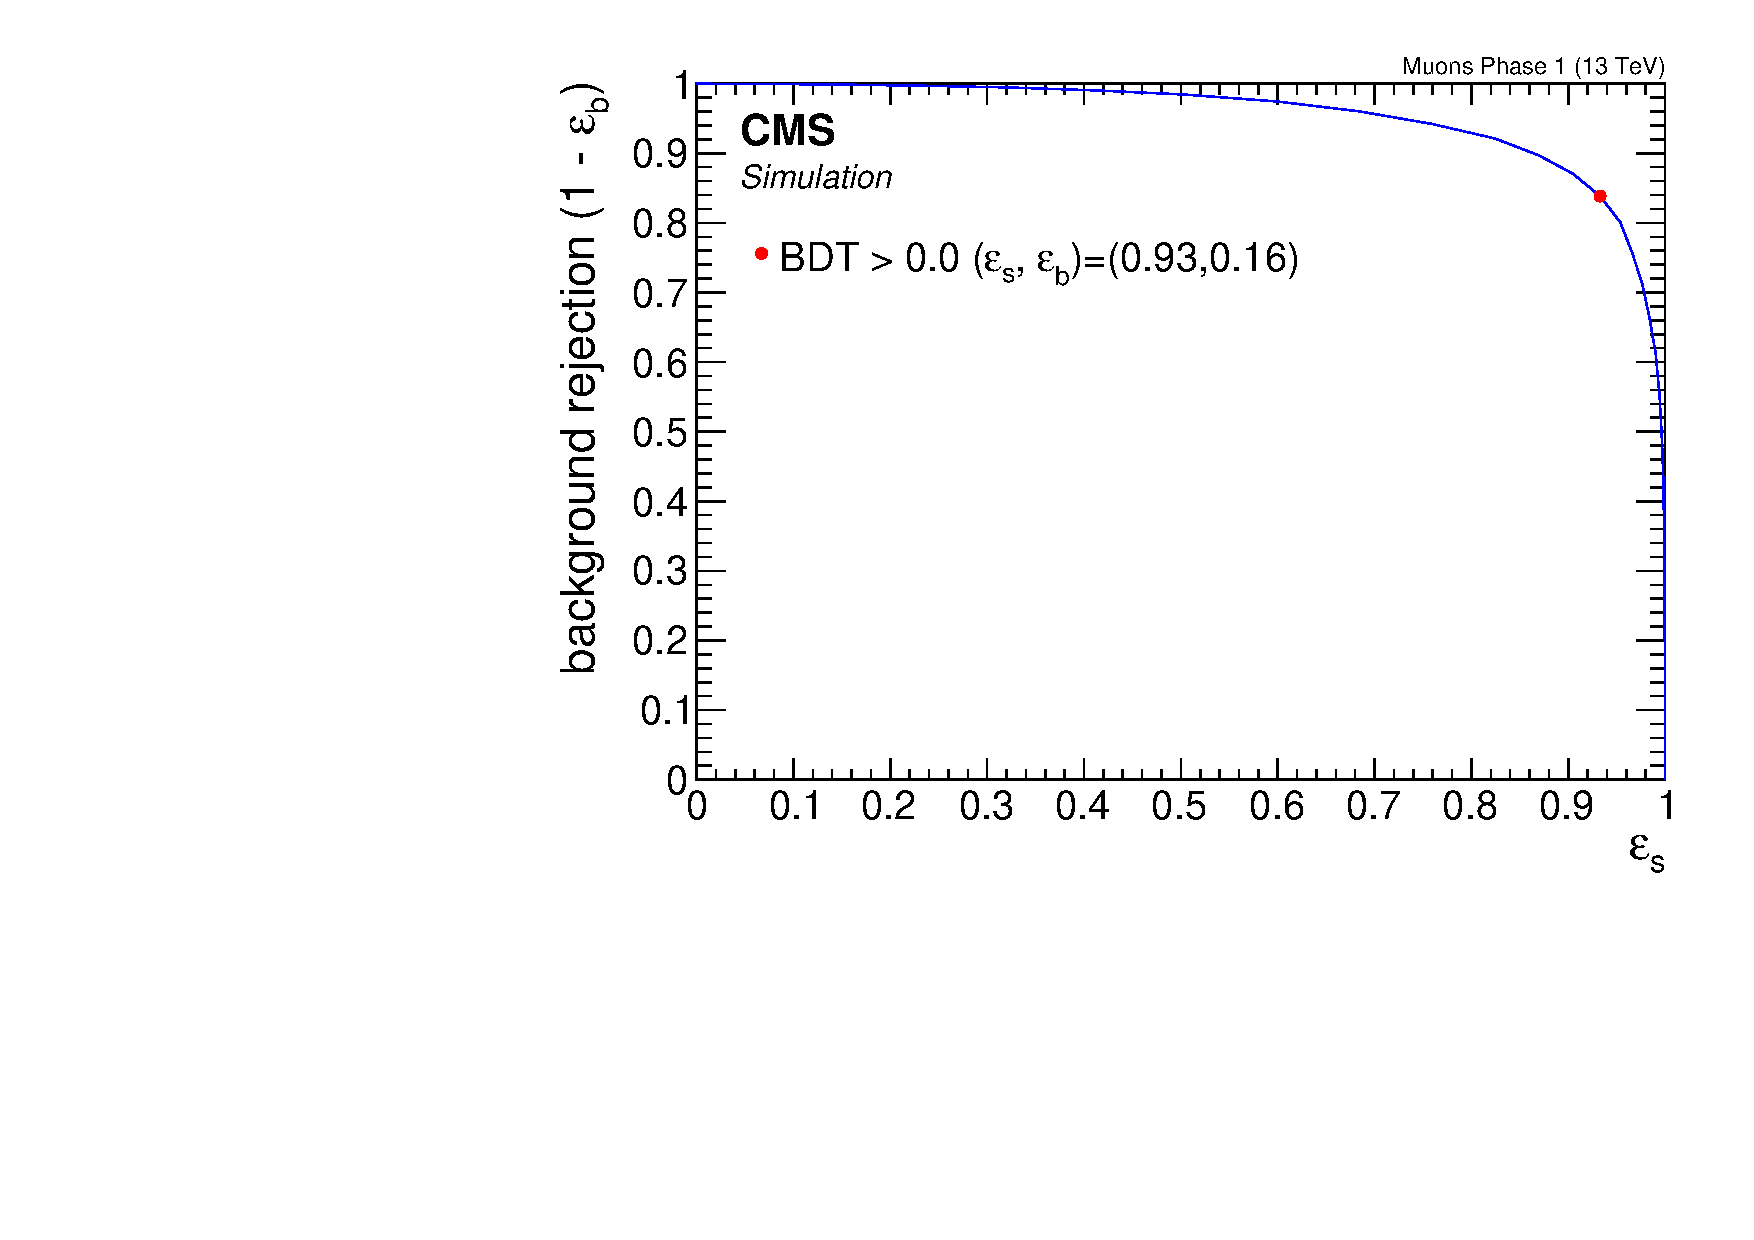
\includegraphics[width=0.48\linewidth]{plots/dimuon_bdt/roc_Event_Dilepton_Muons_Phase_1.pdf} \\


\caption[Dimuon BDT output and ROC curve]{Dimuon BDT output (left) and ROC curve (right).}
\label{fig:event-bdt-dimuon-output}
\end{figure}

\begin{table}[!htb]
	\centering
	\label{tab:dimuon-bdt-variables}
		\caption{Dimuon BDT input variables ranked in order of importance, as reported in the TMVA performance summary table.}
		%\vspace{1mm}
			\begin{tabular}{cll} \hline
			Rank & Variable & Description \\ \hline
			1 & $\mll$ & invariant mass \\
			2 & $\pt(\ell_1)$ & leading lepton \pt\\
			3 & \mht & \\
			4 & \HT & \\
			5 & $\DR\left(\ell\ell\right)$ & \\
			6 & $\mindphimhtjets$ & \\
			7 & $\pt(\vec{\ell}_1+\vec{\ell}_2)$ & dilepton \pt \\
			
			8 & $\pt(\text{leading jet})$ & \\		
			9 & $\pt(\ell_2)$ & subleading lepton \pt \\
			10 & $\eta(\ell_1)$ & leading lepton $\eta$ \\
			11 & $m_T(\ell_1)$ & leading lepton transverse mass\\
			
			12 & $\abs{\Delta\phi\left(\ell_2, \htvecmiss \right)}$ & \\
			13 & $\abs{\Delta\phi\left(\ell_1, \htvecmiss \right)}$ & \\			
			14 & $\abs{\Delta\phi\left(\ell\ell \right)}$ & \\			
			15 & $\njets$ & Number of jets \\ 
			16 & $\eta(\text{leading jet})$ & \\
			17 & $\abs{\Delta \eta \left(\ell \ell\right) }$ & \\
			18 & $\mtautau$ & collinear approximation of $\mtautau$\\
			\hline
			\end{tabular}
\end{table}

Distributions of the input variables to the \gls{bdt} are shown in Figure~\ref{fig:dimuon-input-distributions}.

\begin{figure}[!htb]
\centering
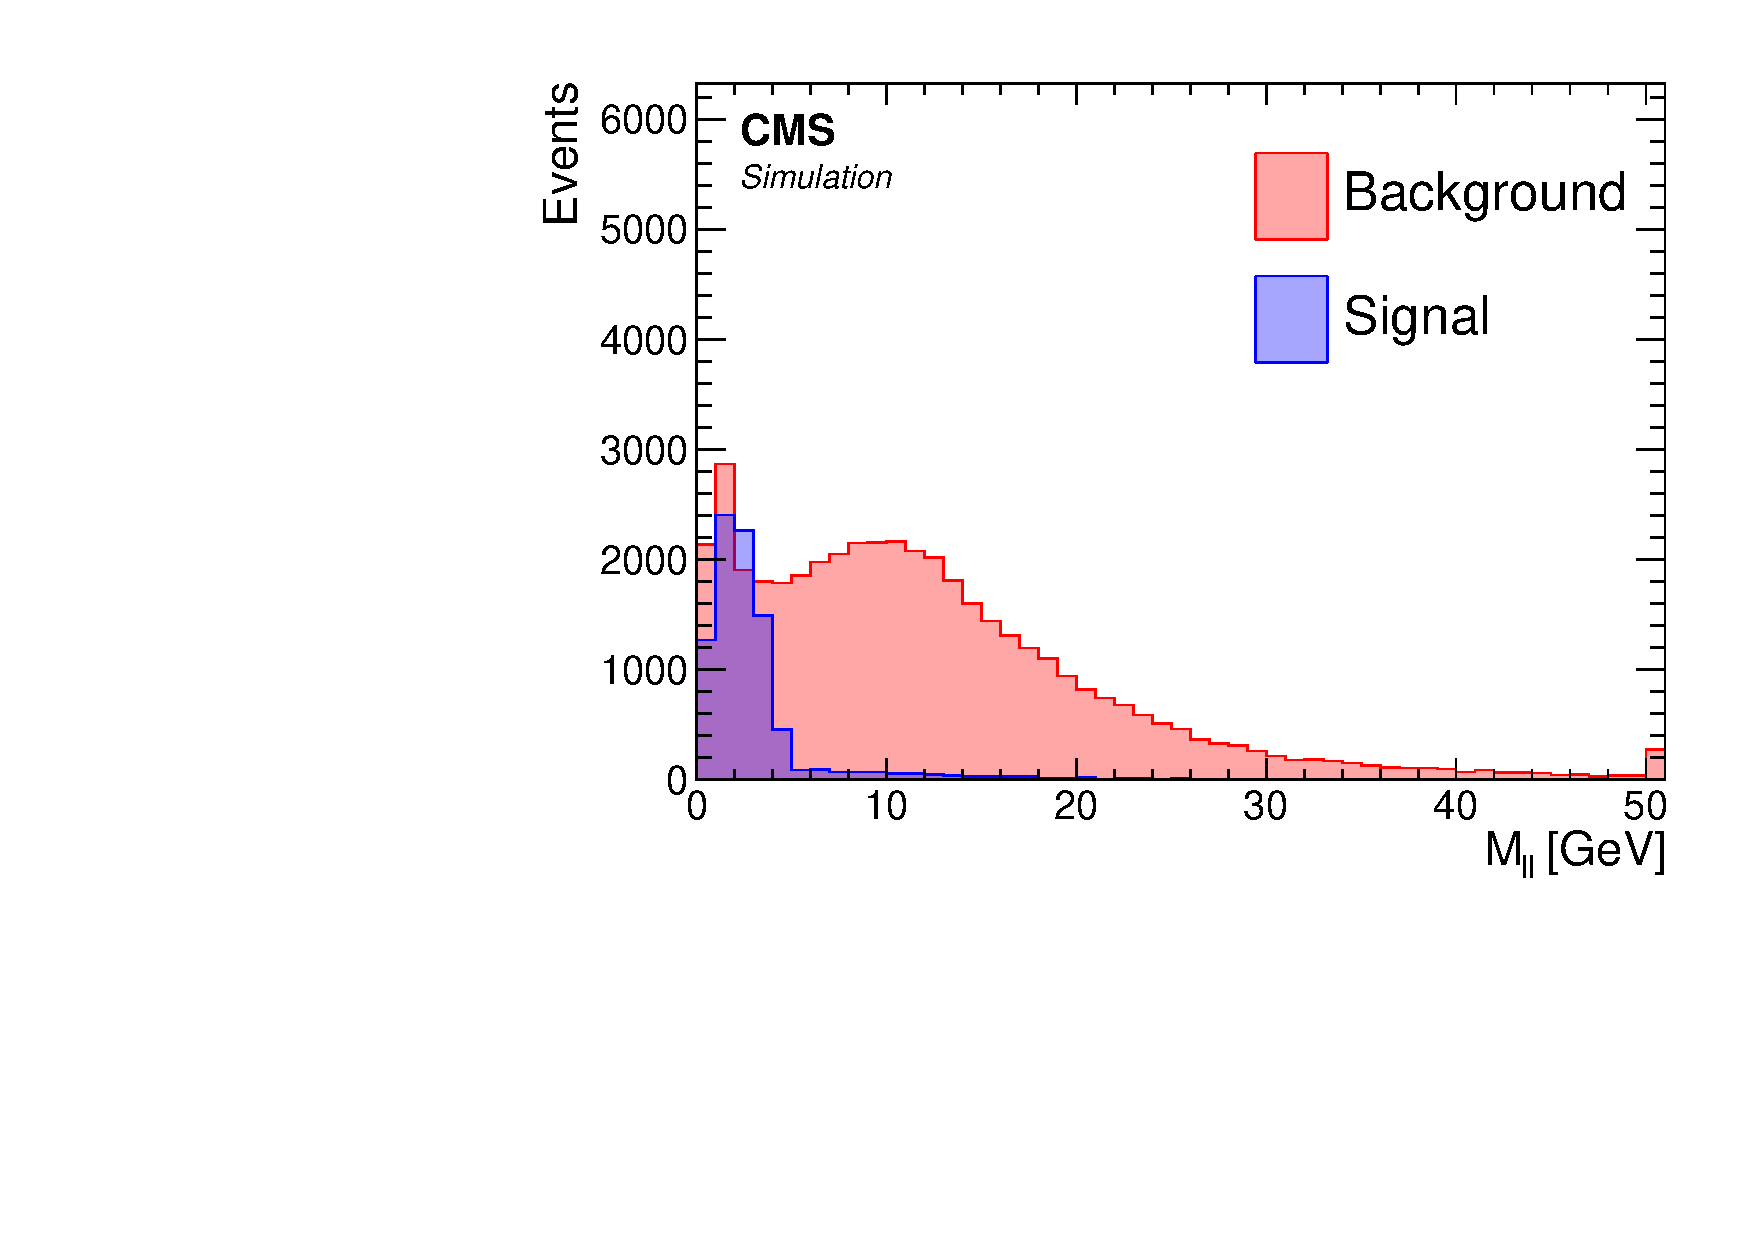
\includegraphics[width=0.32\linewidth]{plots/dilepton_bdt_inputs_muons/none_invMassCorrJetNoMultIso10Dr0.6.pdf} \,
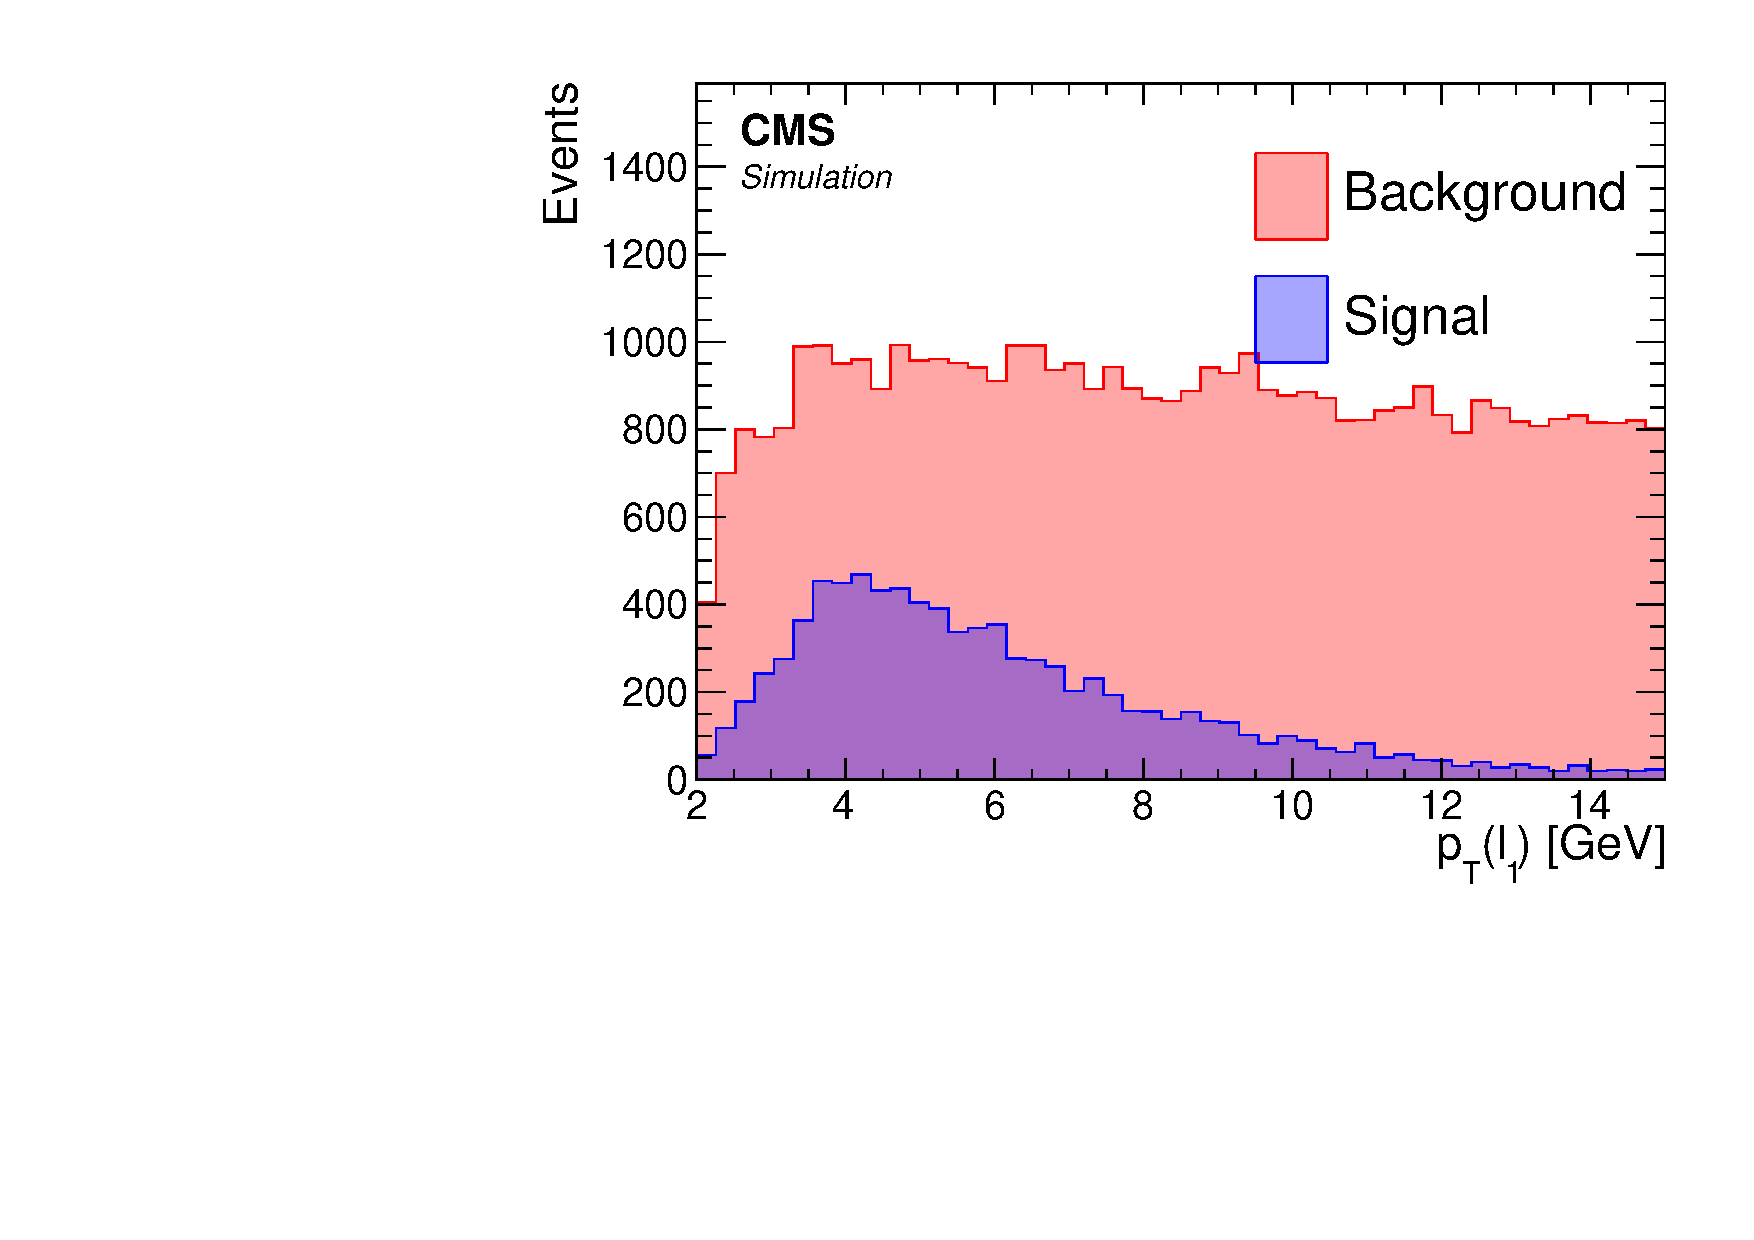
\includegraphics[width=0.32\linewidth]{plots/dilepton_bdt_inputs_muons/none_leptonsCorrJetNoMultIso10Dr0.6_0_.Pt__.pdf} \,
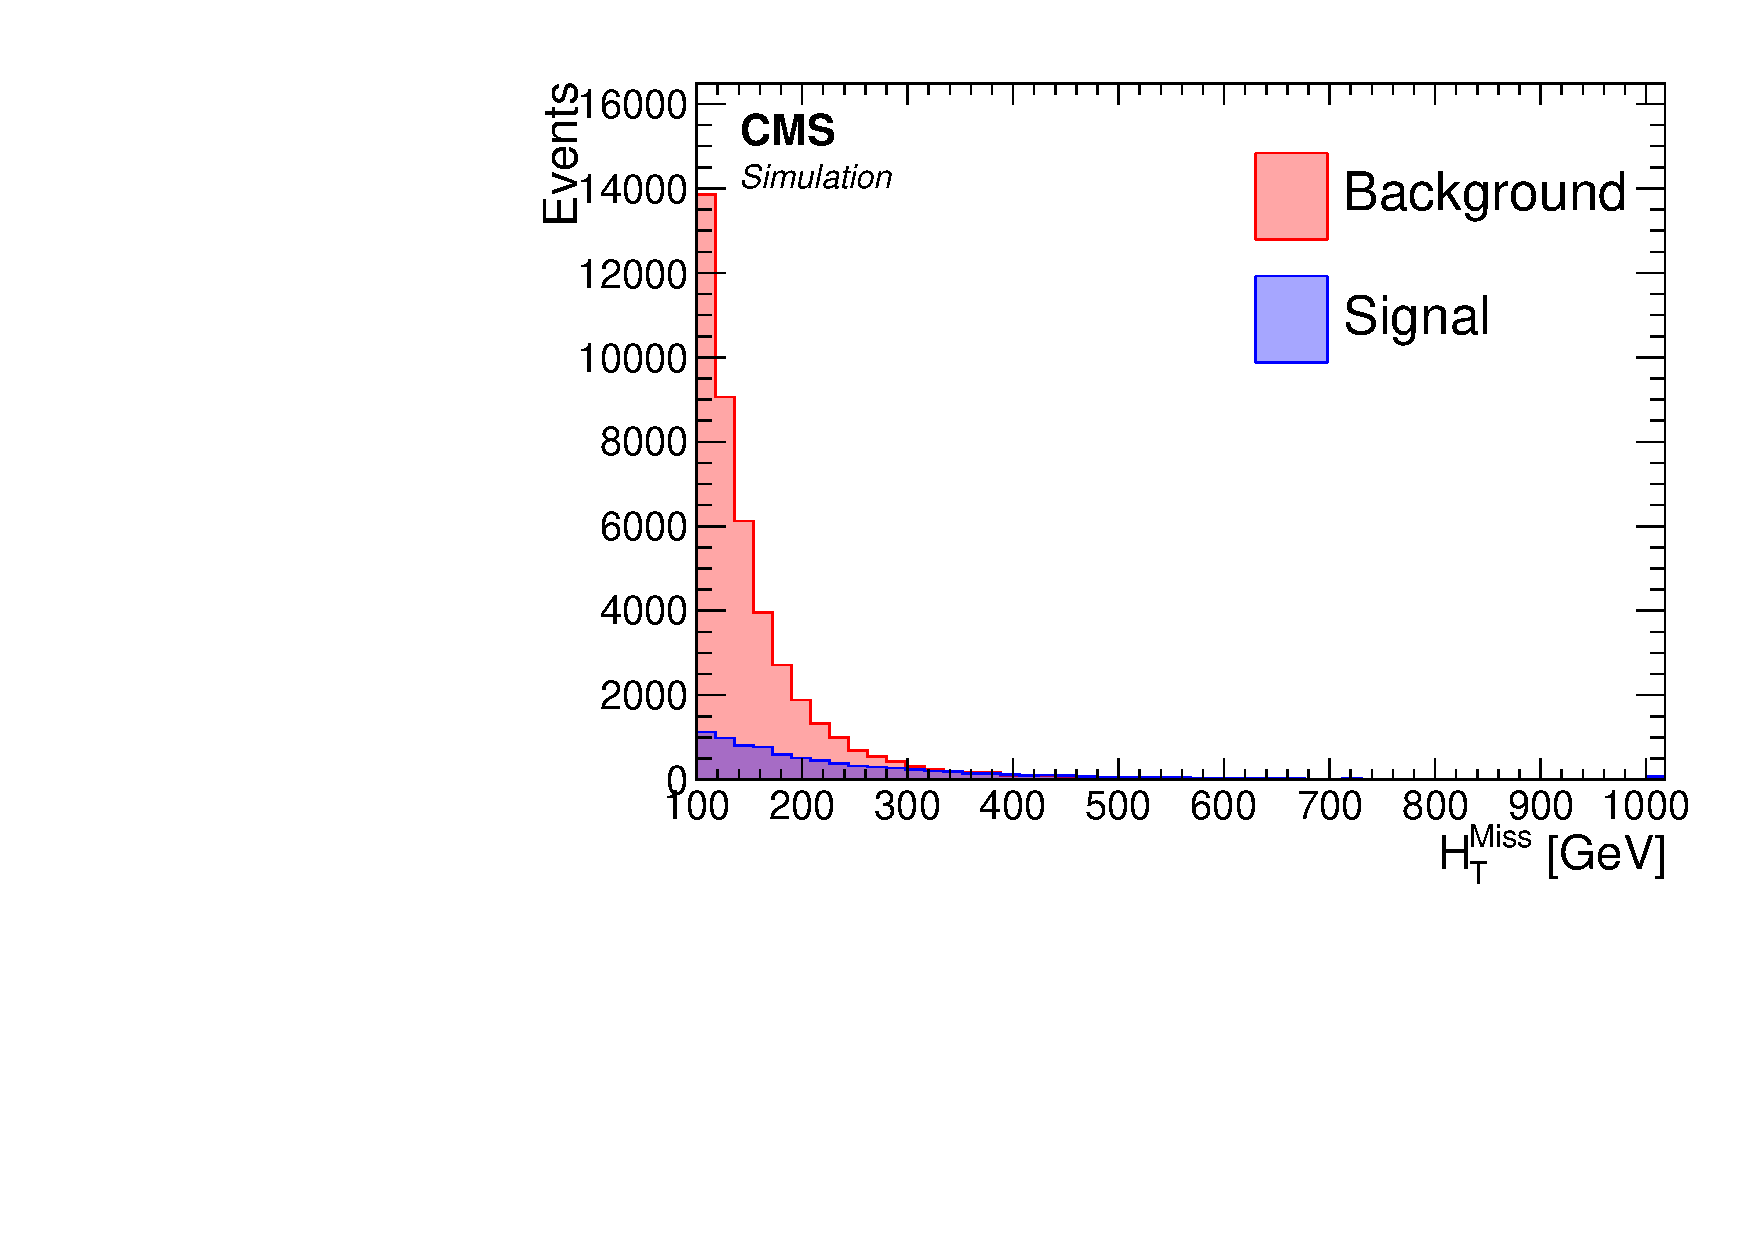
\includegraphics[width=0.32\linewidth]{plots/dilepton_bdt_inputs_muons/none_MHT.pdf}   \\
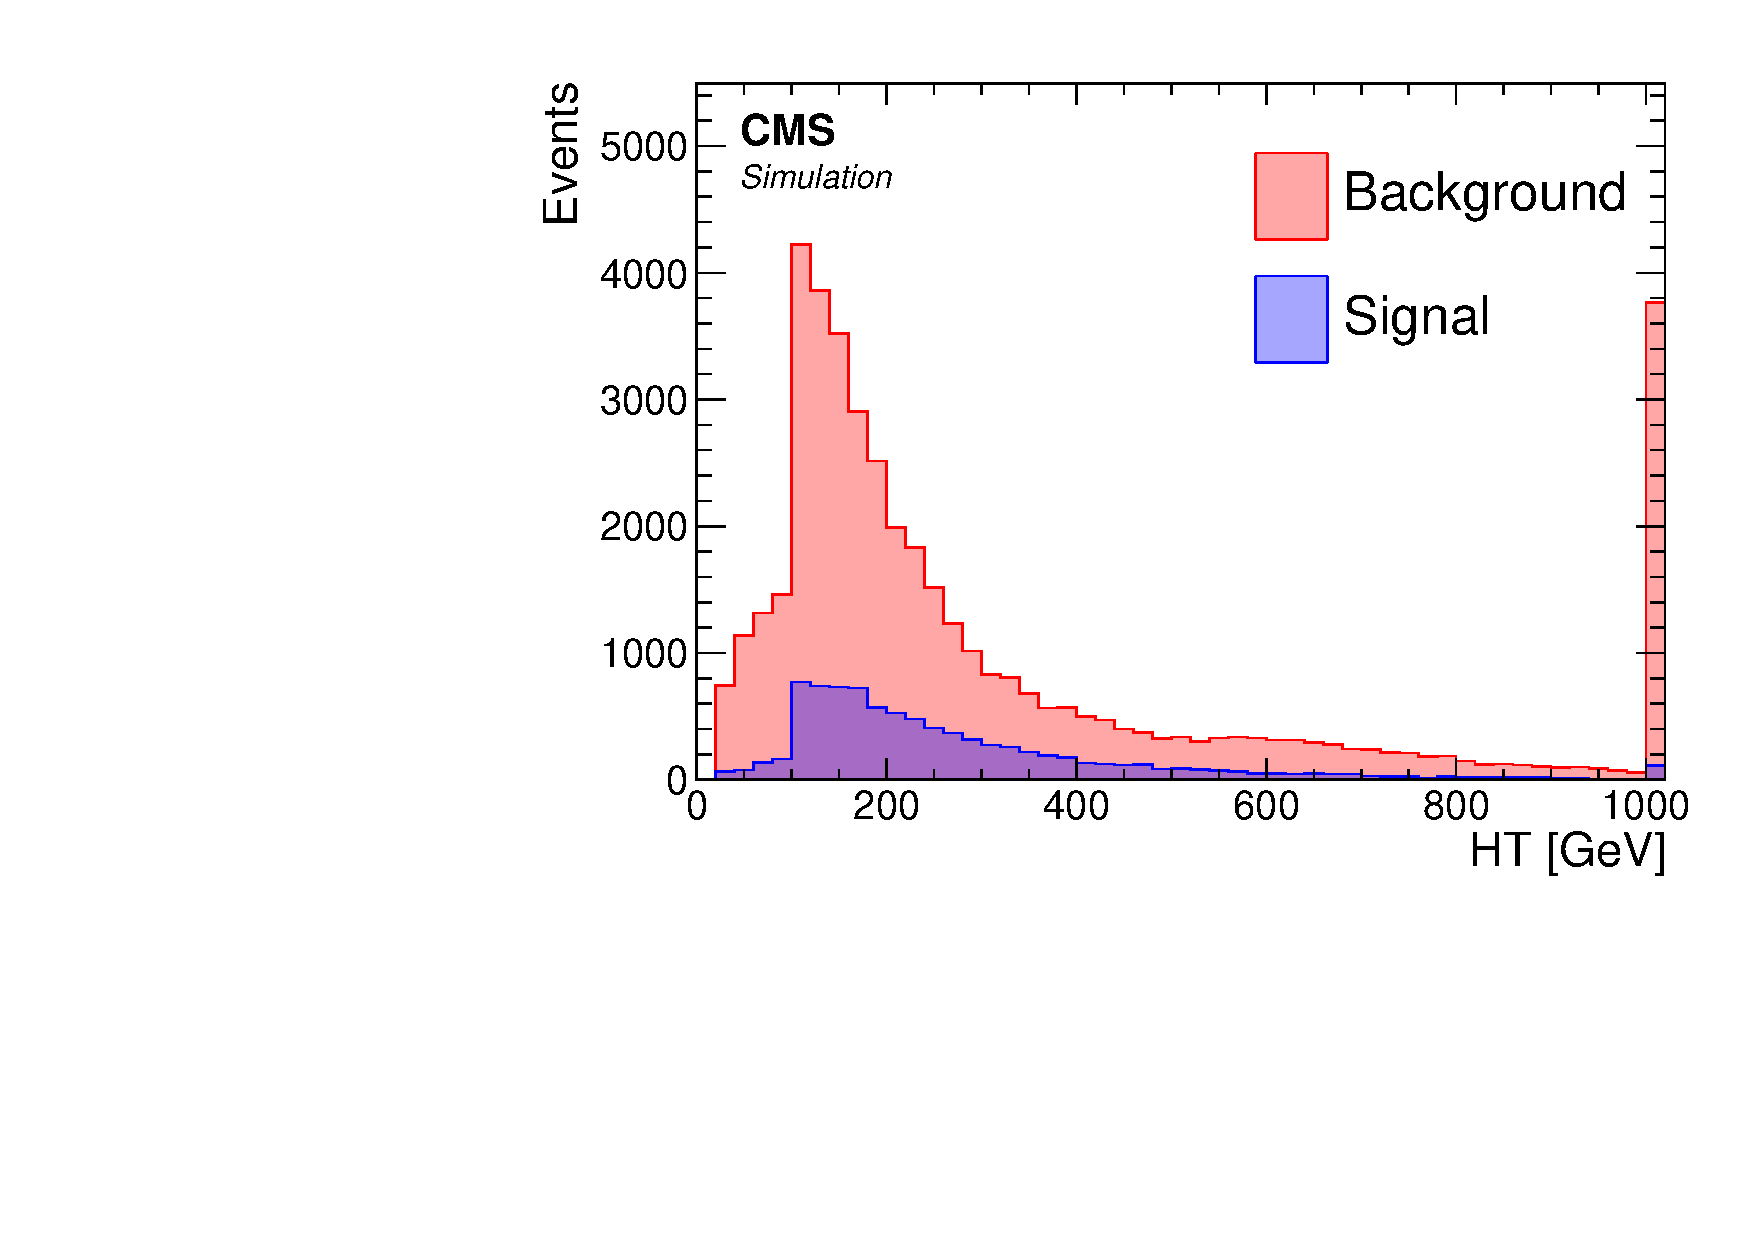
\includegraphics[width=0.32\linewidth]{plots/dilepton_bdt_inputs_muons/none_HT.pdf} \,
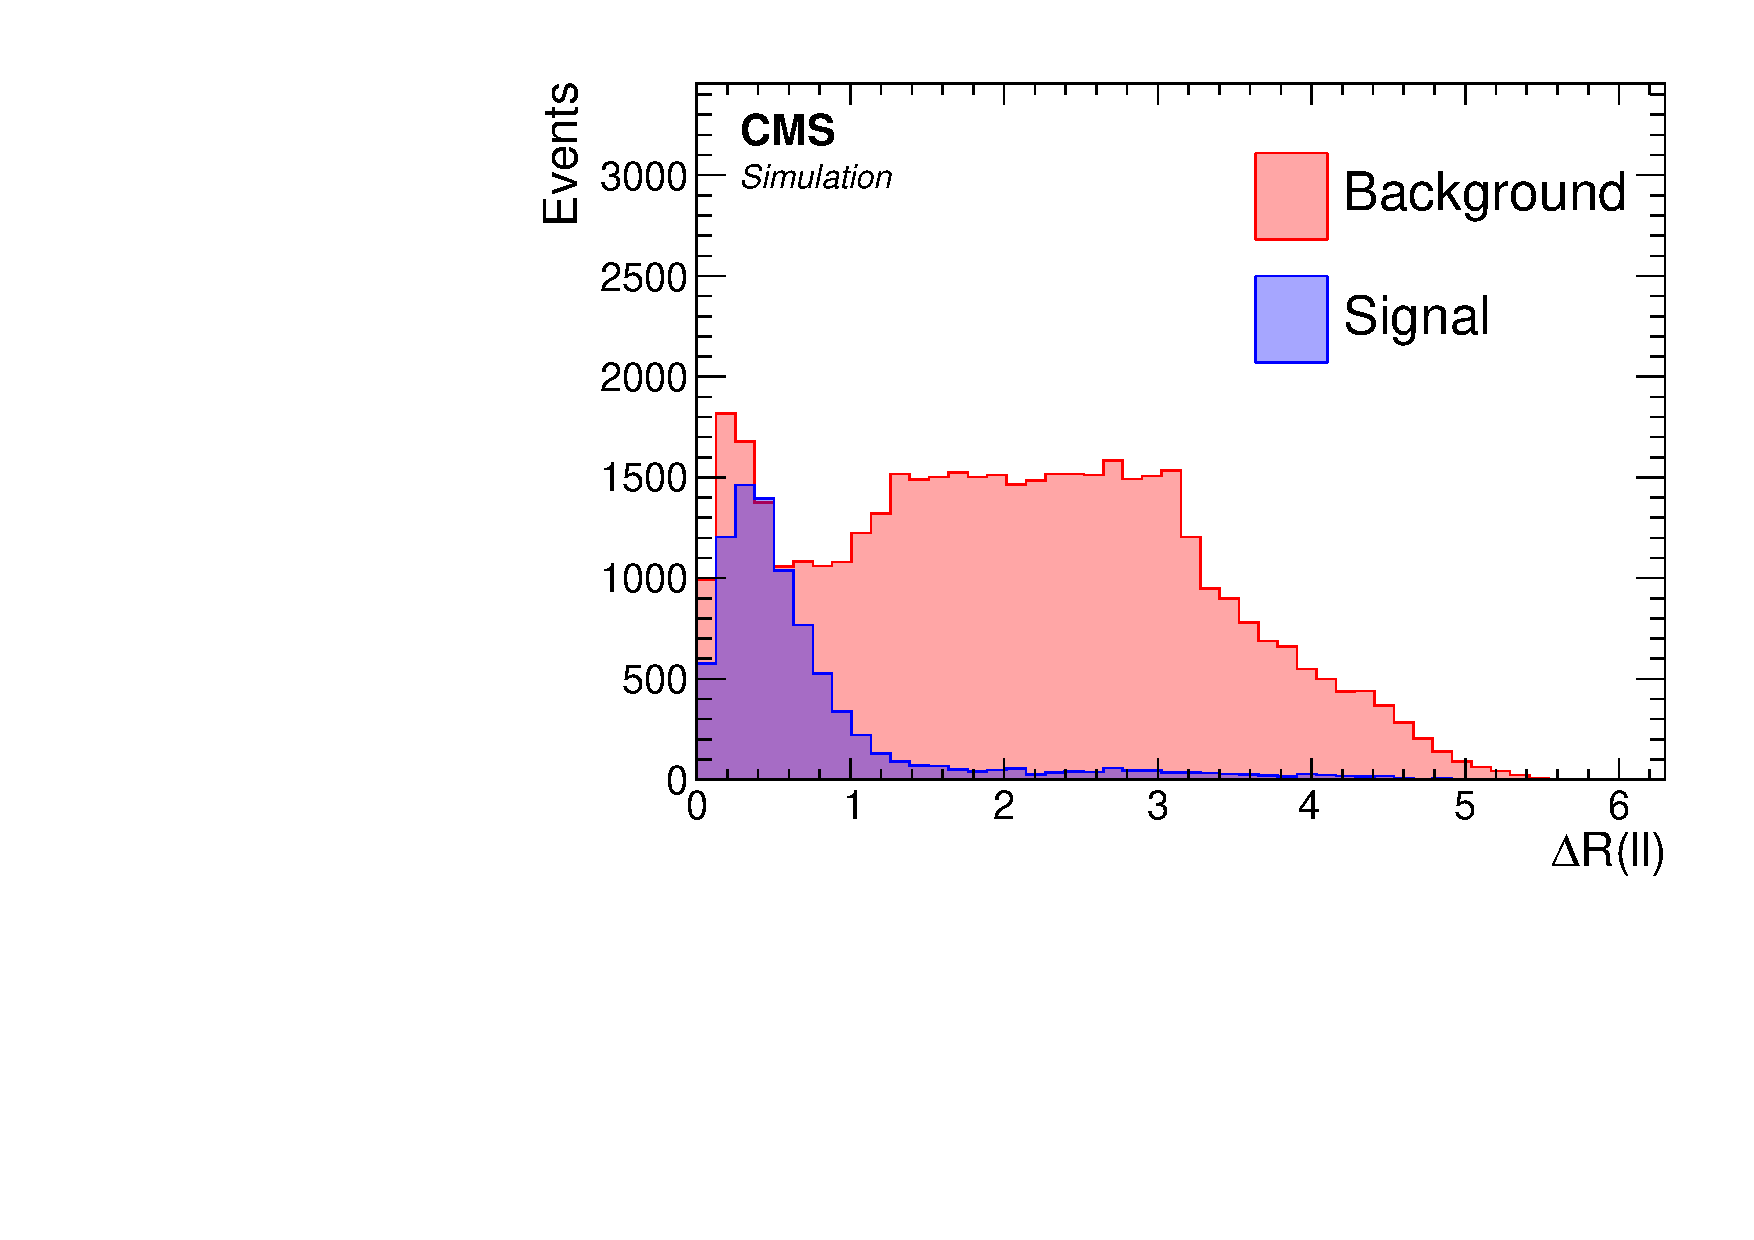
\includegraphics[width=0.32\linewidth]{plots/dilepton_bdt_inputs_muons/none_deltaRCorrJetNoMultIso10Dr0.6.pdf}  \,
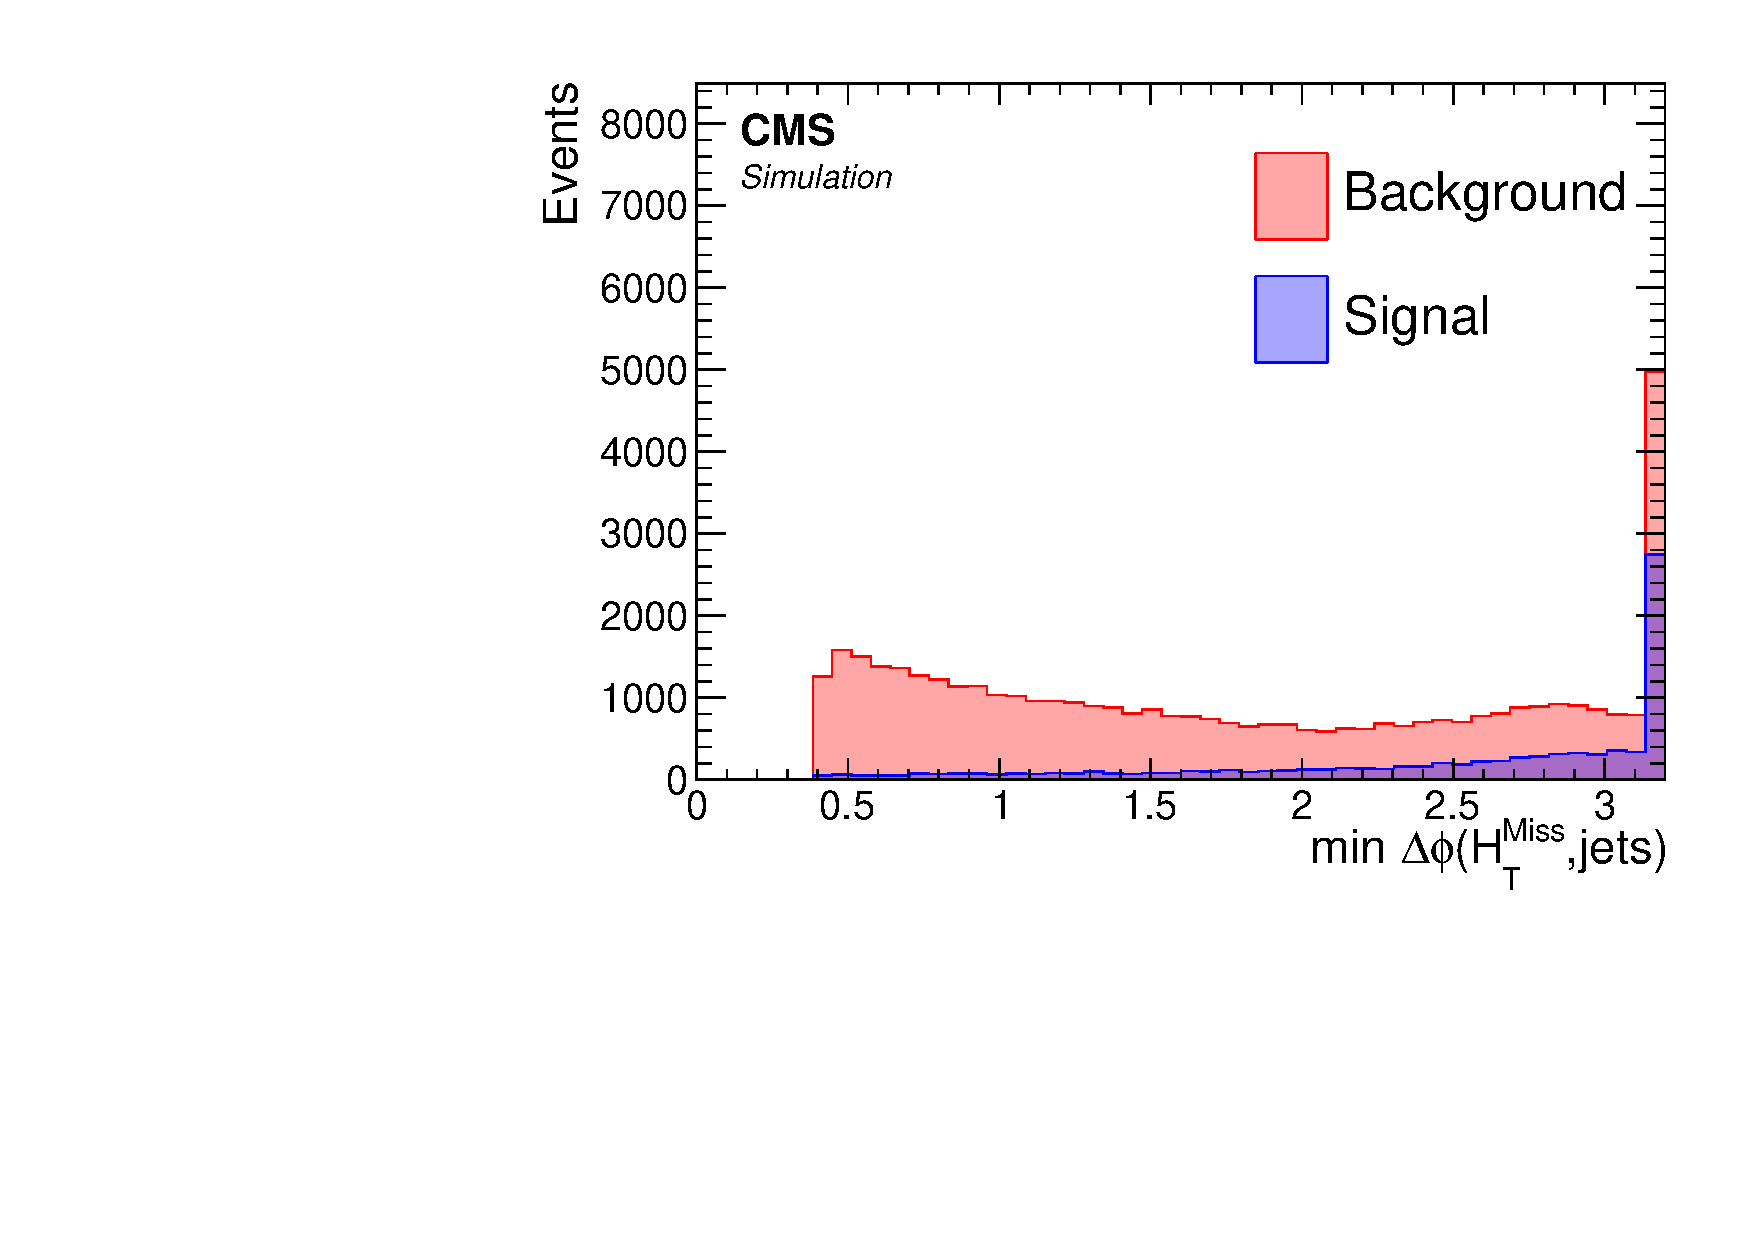
\includegraphics[width=0.32\linewidth]{plots/dilepton_bdt_inputs_muons/none_MinDeltaPhiMhtJets.pdf} \\


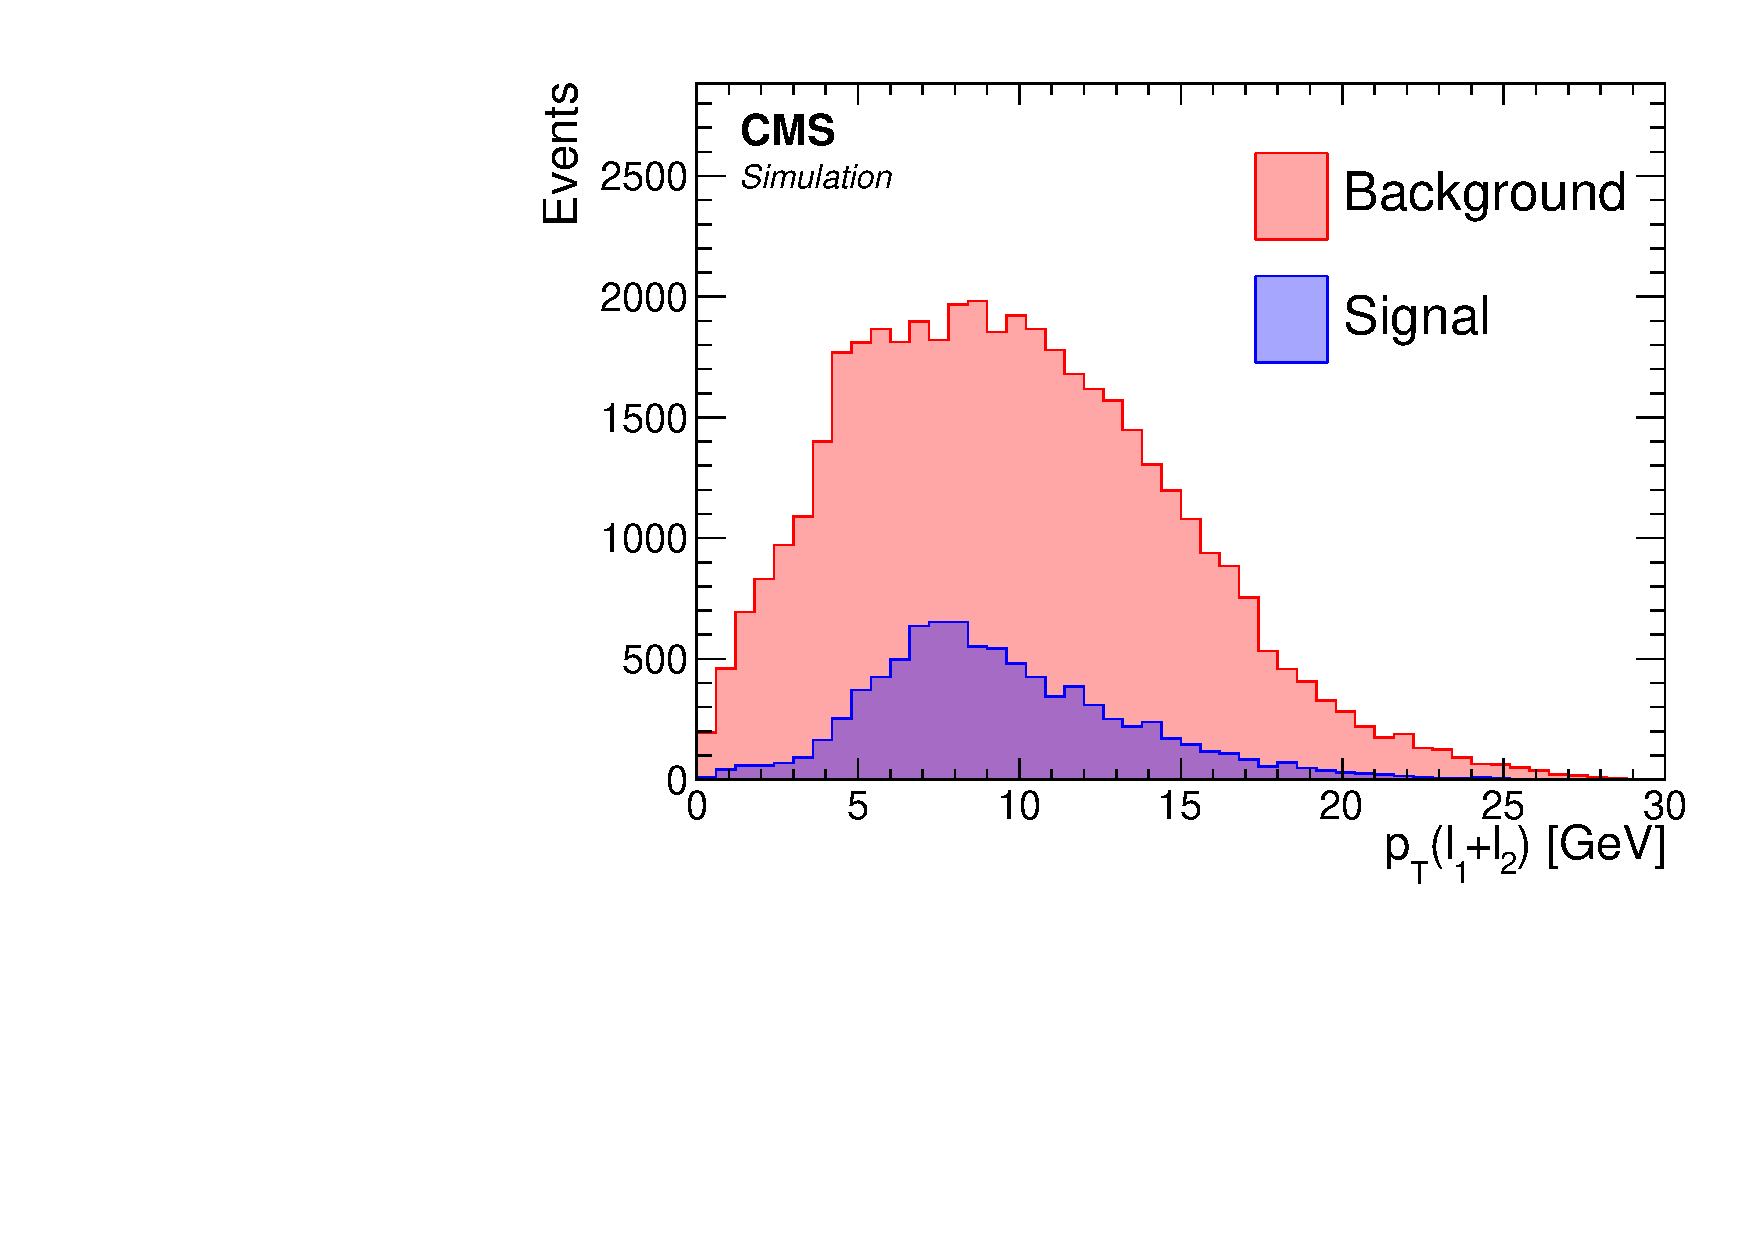
\includegraphics[width=0.32\linewidth]{plots/dilepton_bdt_inputs_muons/none_dileptonPtCorrJetNoMultIso10Dr0.6.pdf} \,
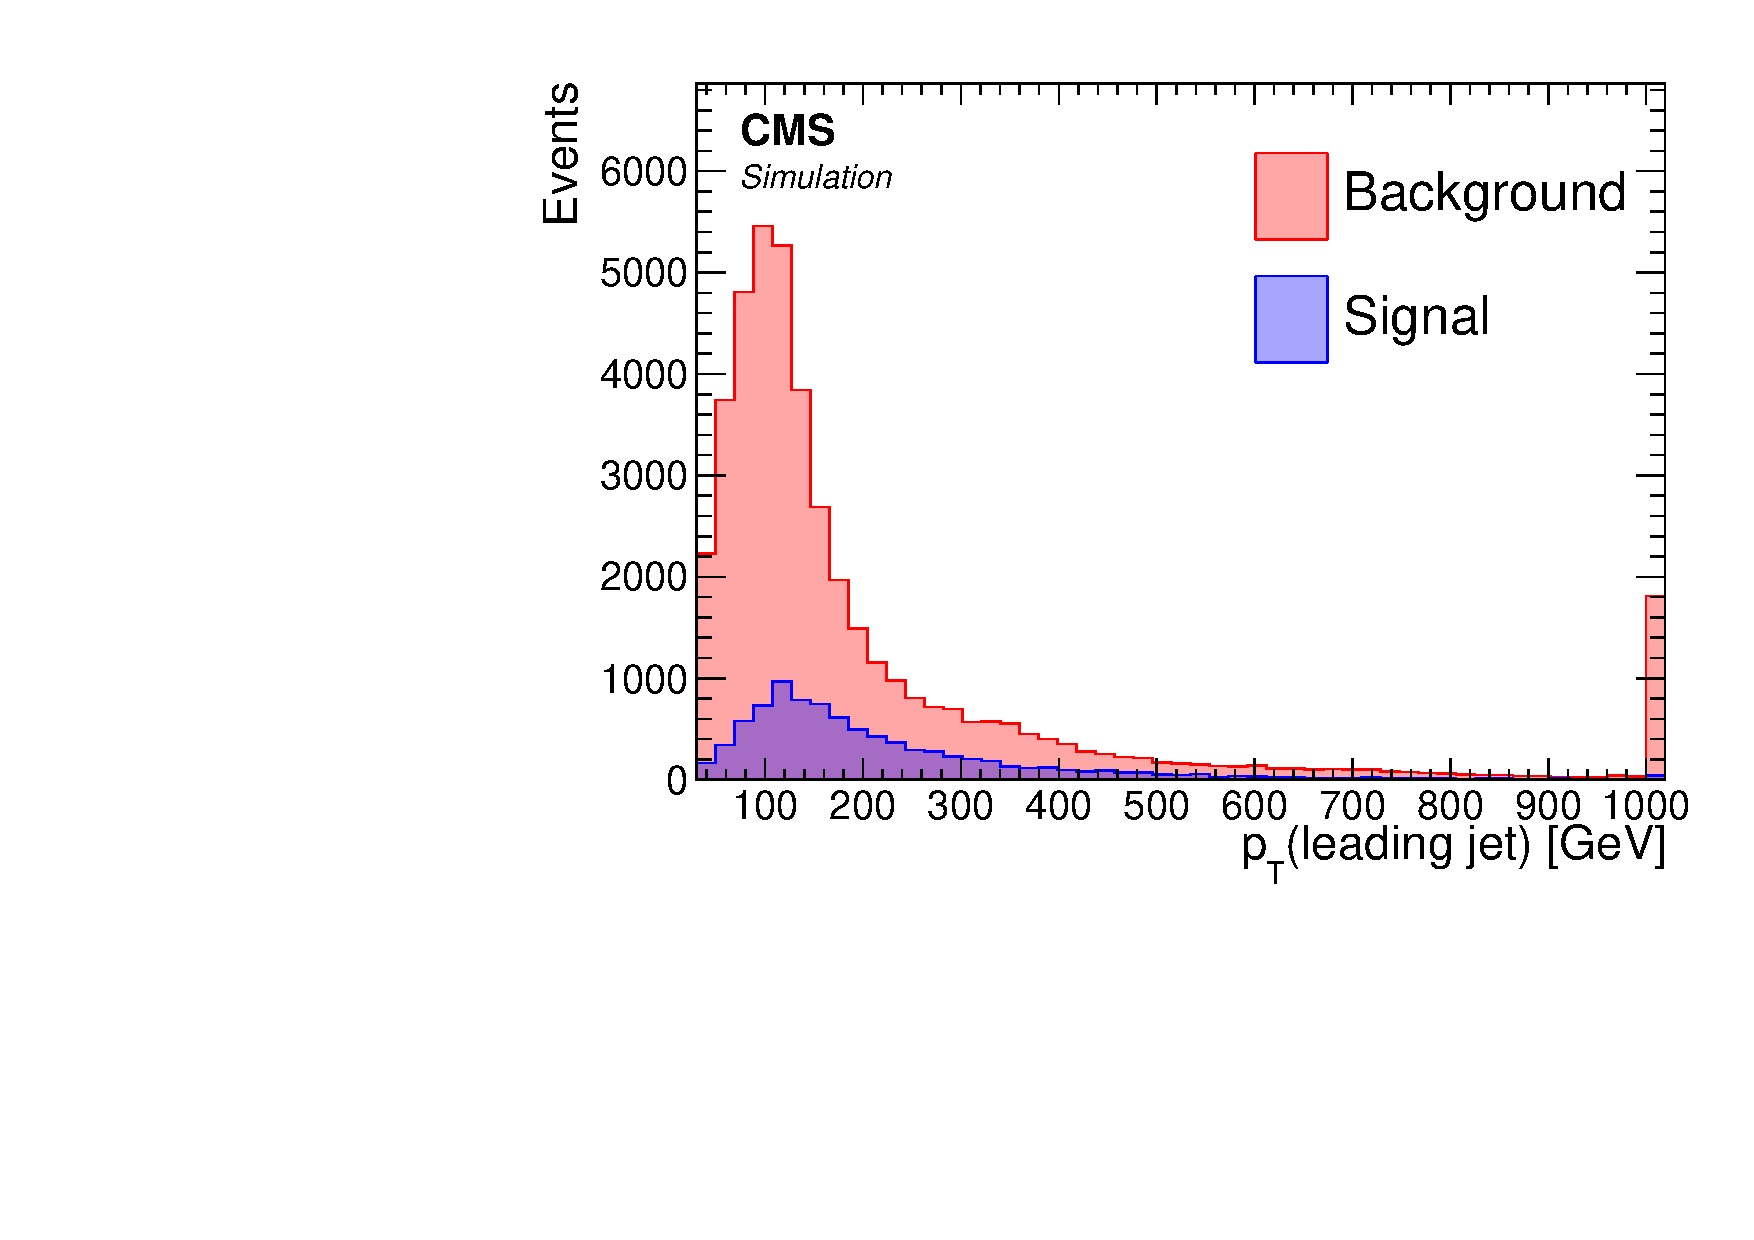
\includegraphics[width=0.32\linewidth]{plots/dilepton_bdt_inputs_muons/none_LeadingJetPt.pdf} \,
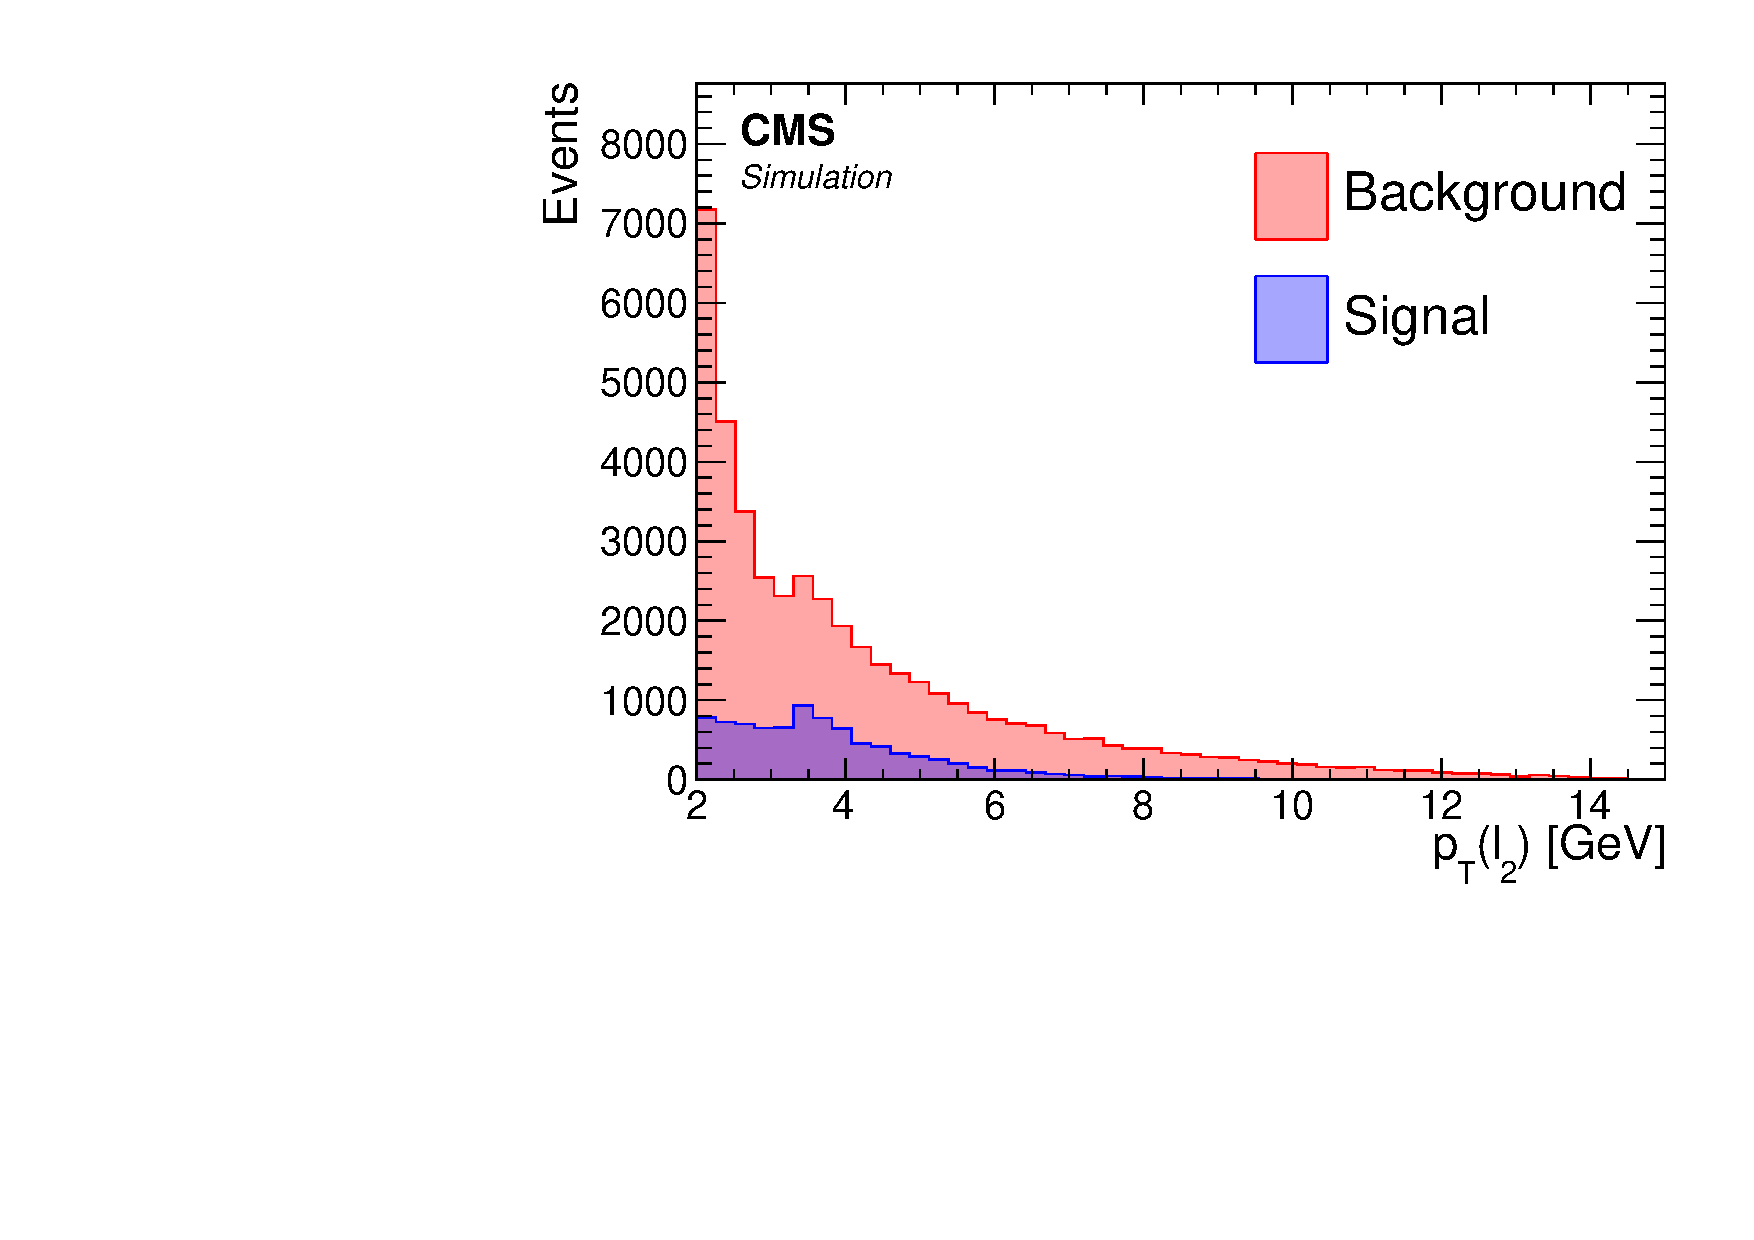
\includegraphics[width=0.32\linewidth]{plots/dilepton_bdt_inputs_muons/none_leptonsCorrJetNoMultIso10Dr0.6_1_.Pt__.pdf}   \\
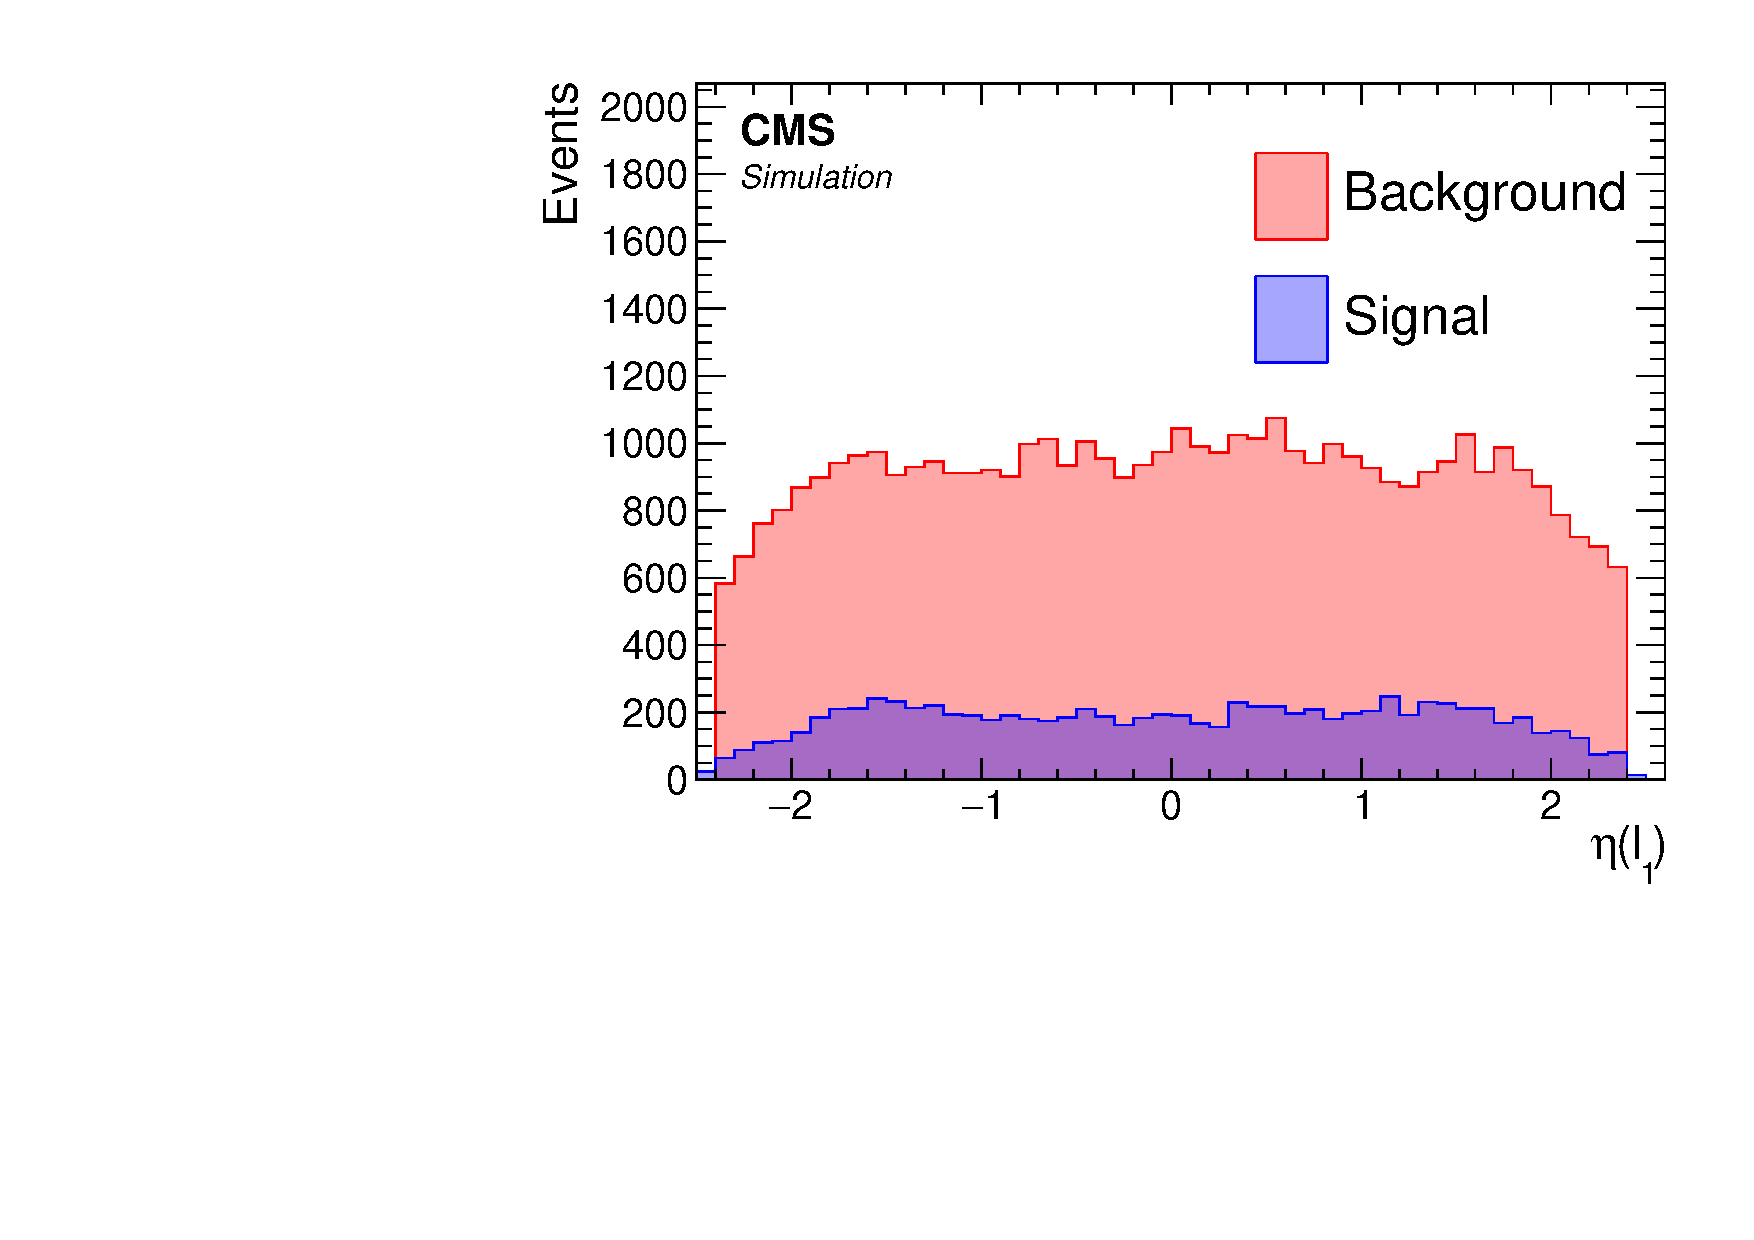
\includegraphics[width=0.32\linewidth]{plots/dilepton_bdt_inputs_muons/none_leptonsCorrJetNoMultIso10Dr0.6_0_.Eta__.pdf} \,
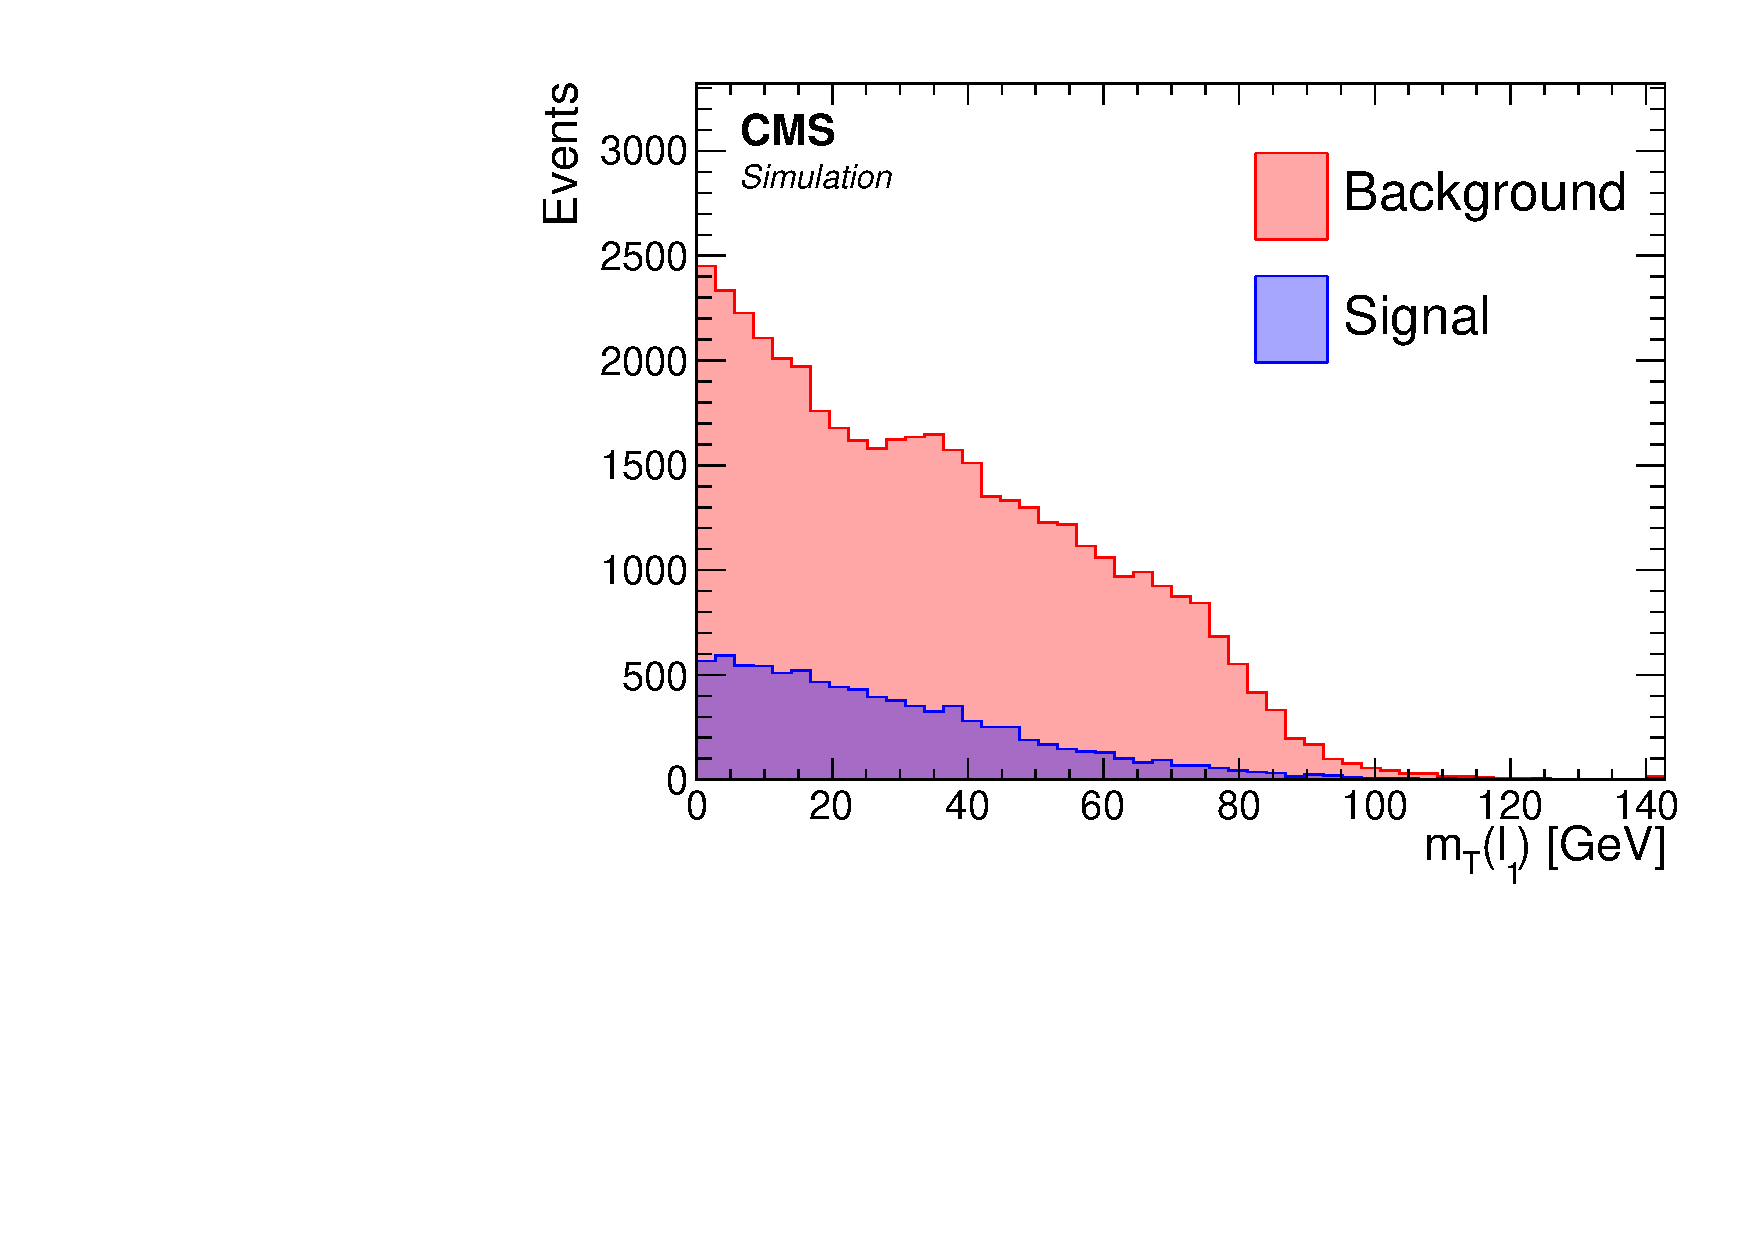
\includegraphics[width=0.32\linewidth]{plots/dilepton_bdt_inputs_muons/none_mth1CorrJetNoMultIso10Dr0.6.pdf}  \,
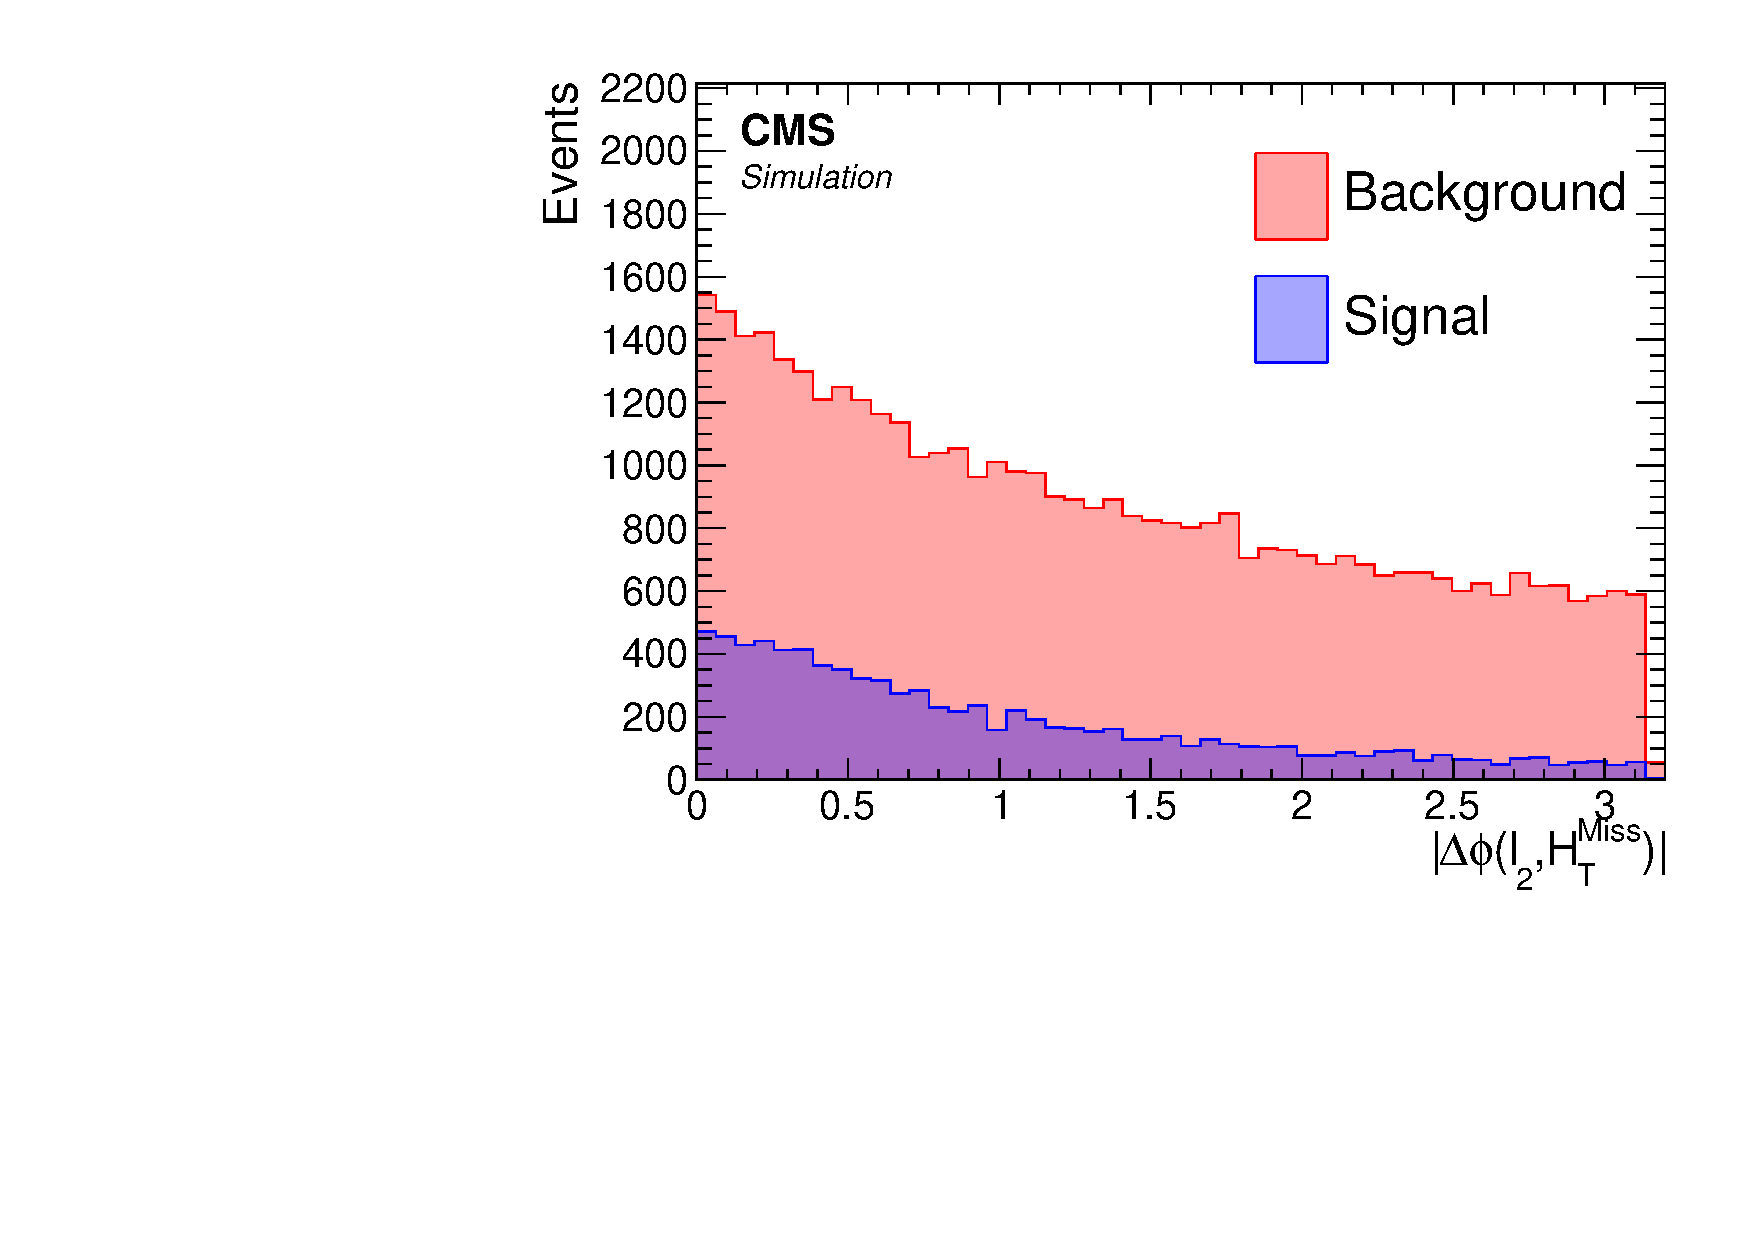
\includegraphics[width=0.32\linewidth]{plots/dilepton_bdt_inputs_muons/none_deltaPhiMhtLepton2CorrJetNoMultIso10Dr0.6.pdf} \\


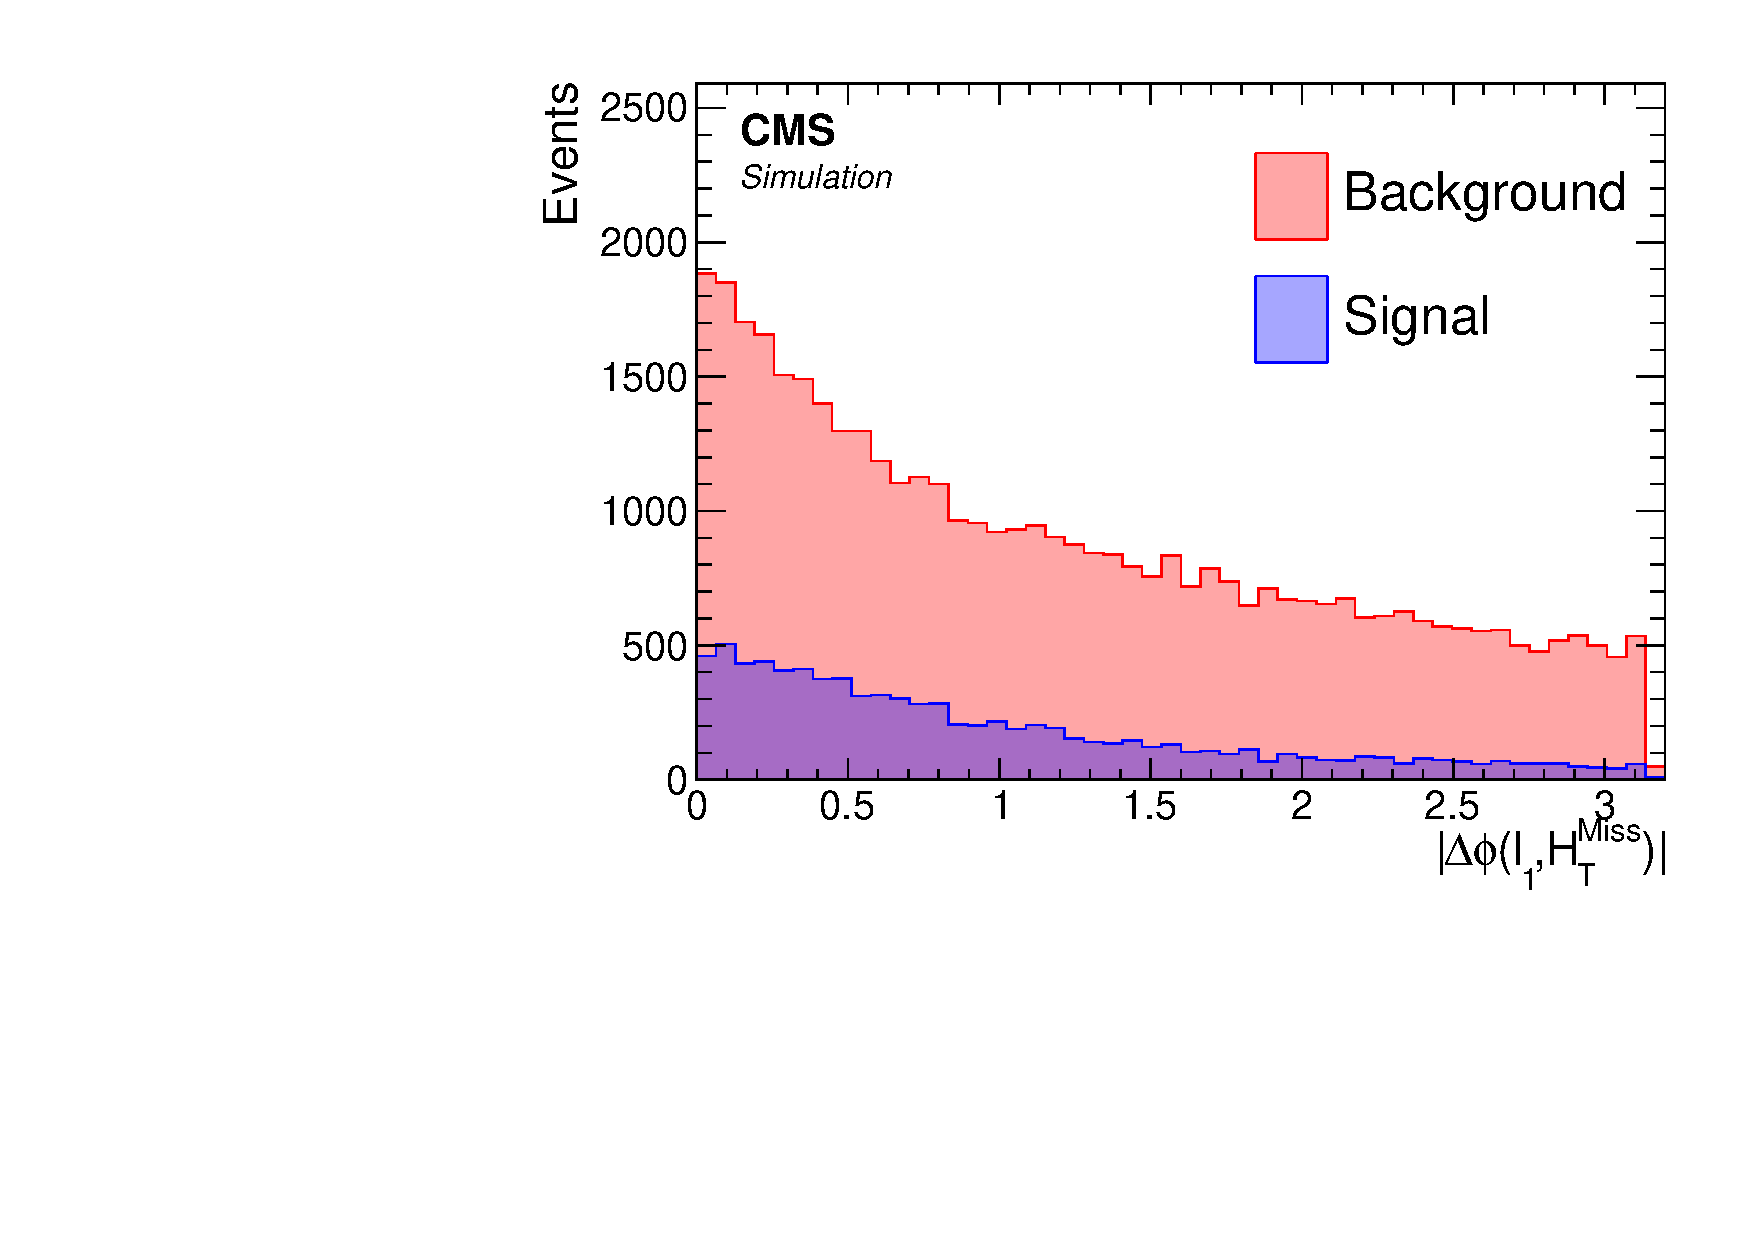
\includegraphics[width=0.32\linewidth]{plots/dilepton_bdt_inputs_muons/none_deltaPhiMhtLepton1CorrJetNoMultIso10Dr0.6.pdf} \,
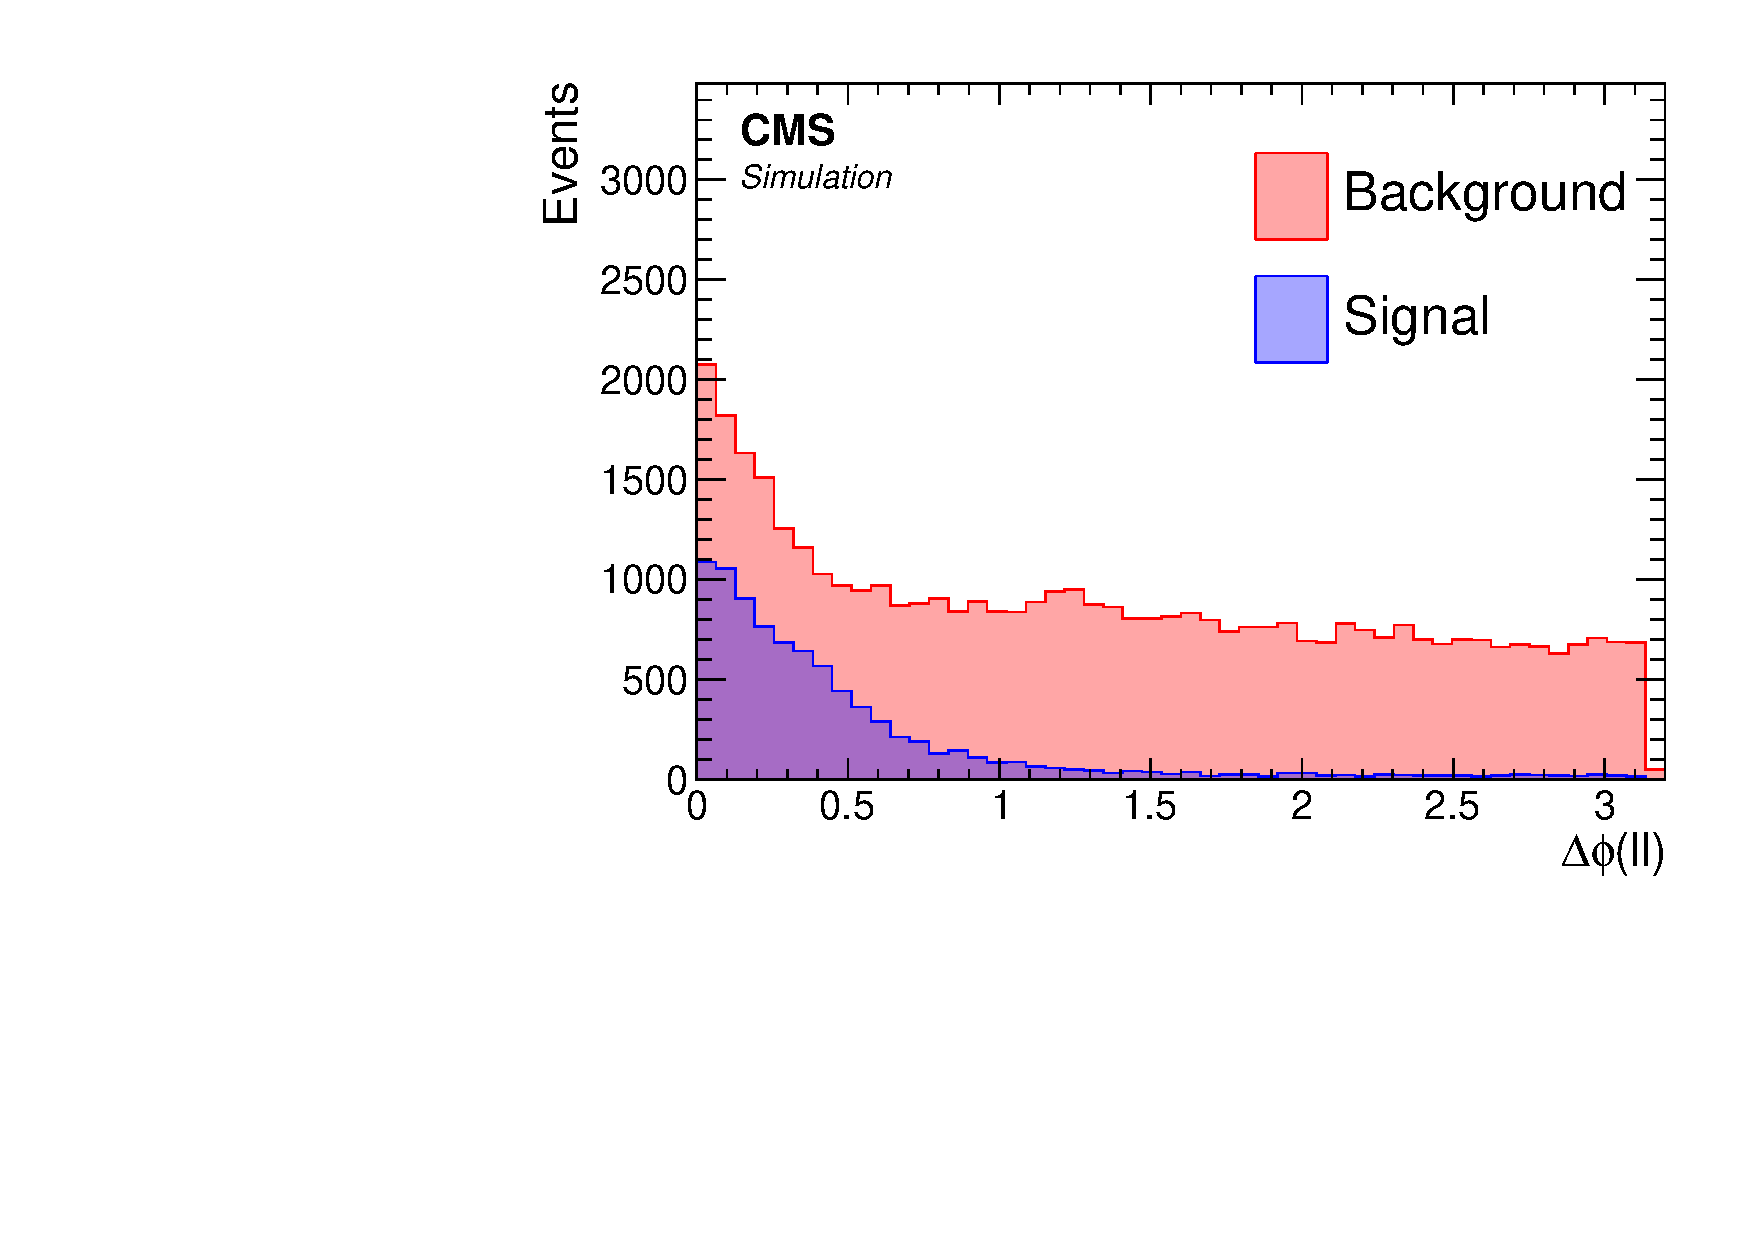
\includegraphics[width=0.32\linewidth]{plots/dilepton_bdt_inputs_muons/none_deltaPhiCorrJetNoMultIso10Dr0.6.pdf} \,
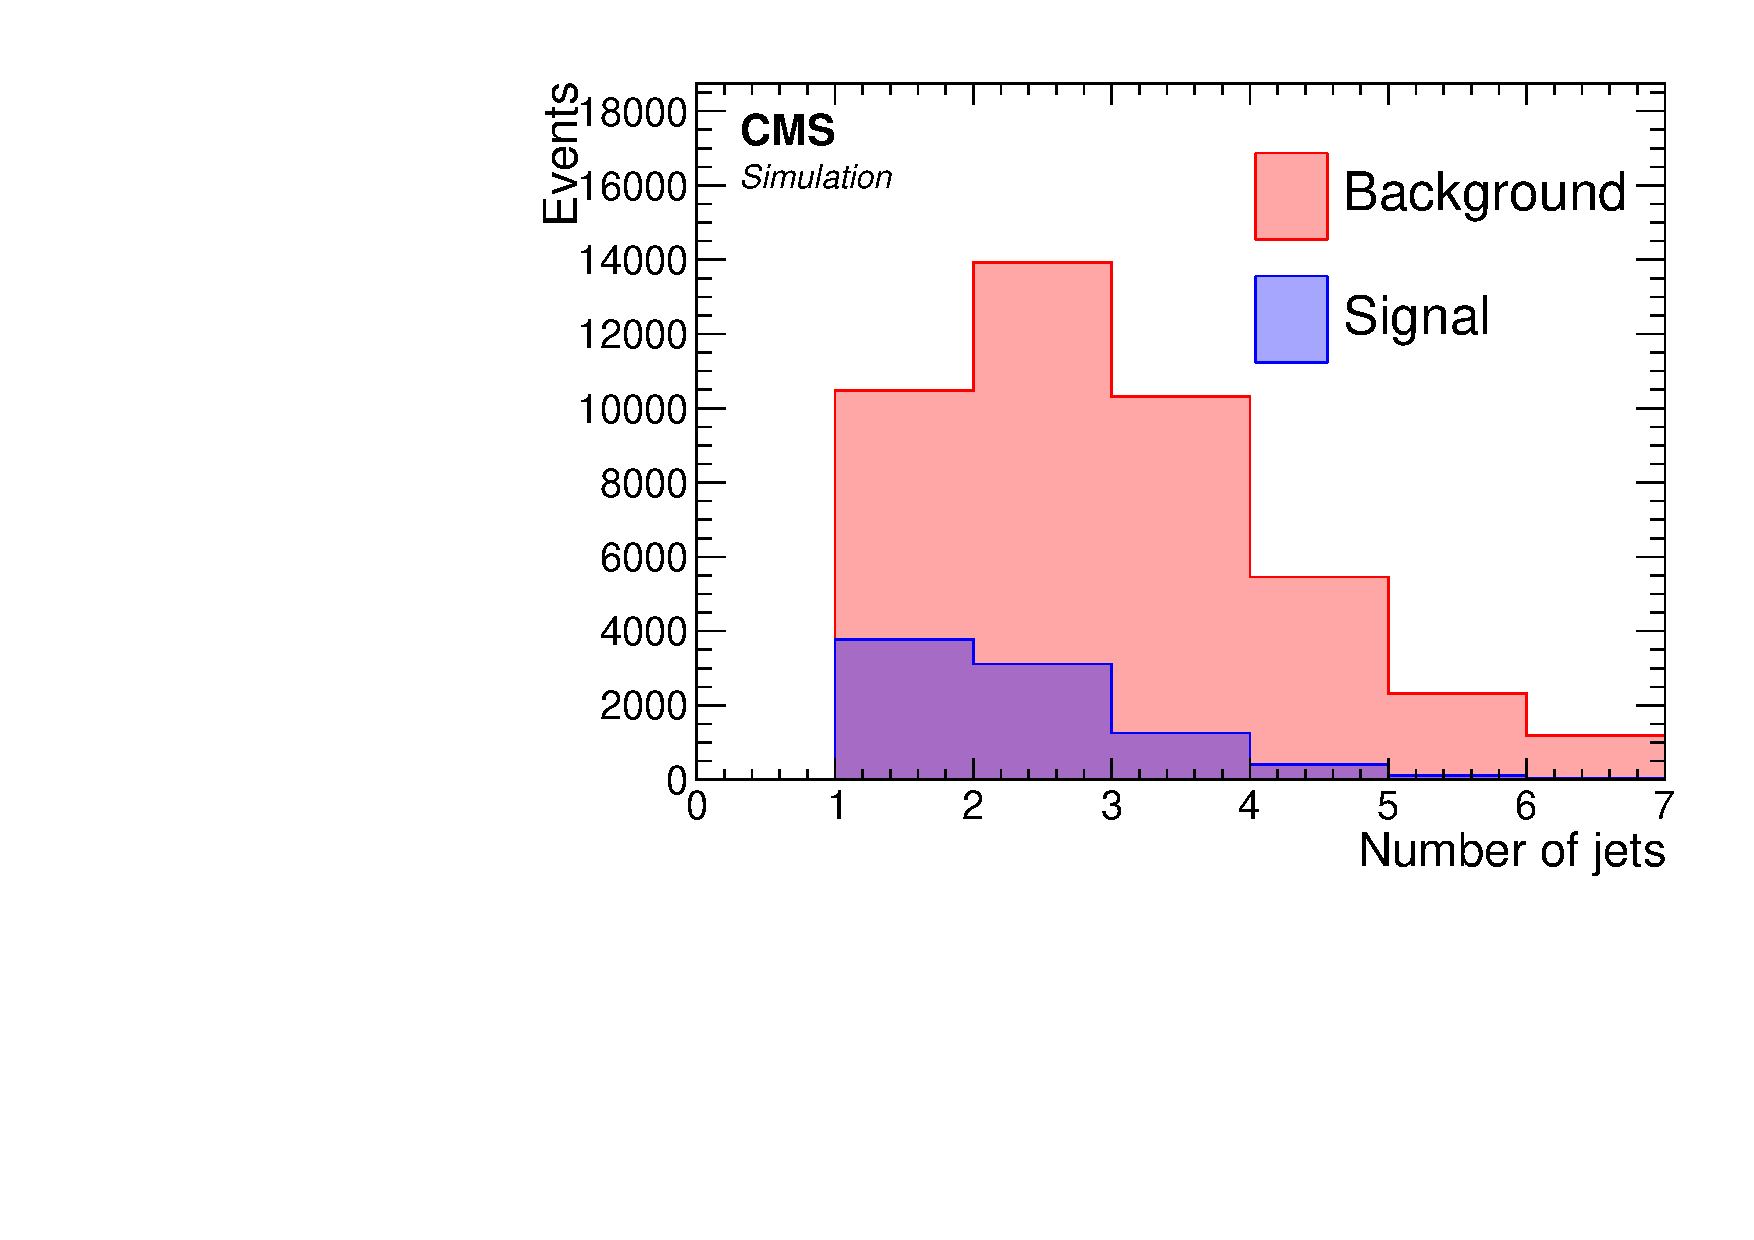
\includegraphics[width=0.32\linewidth]{plots/dilepton_bdt_inputs_muons/none_NJets.pdf}   \\
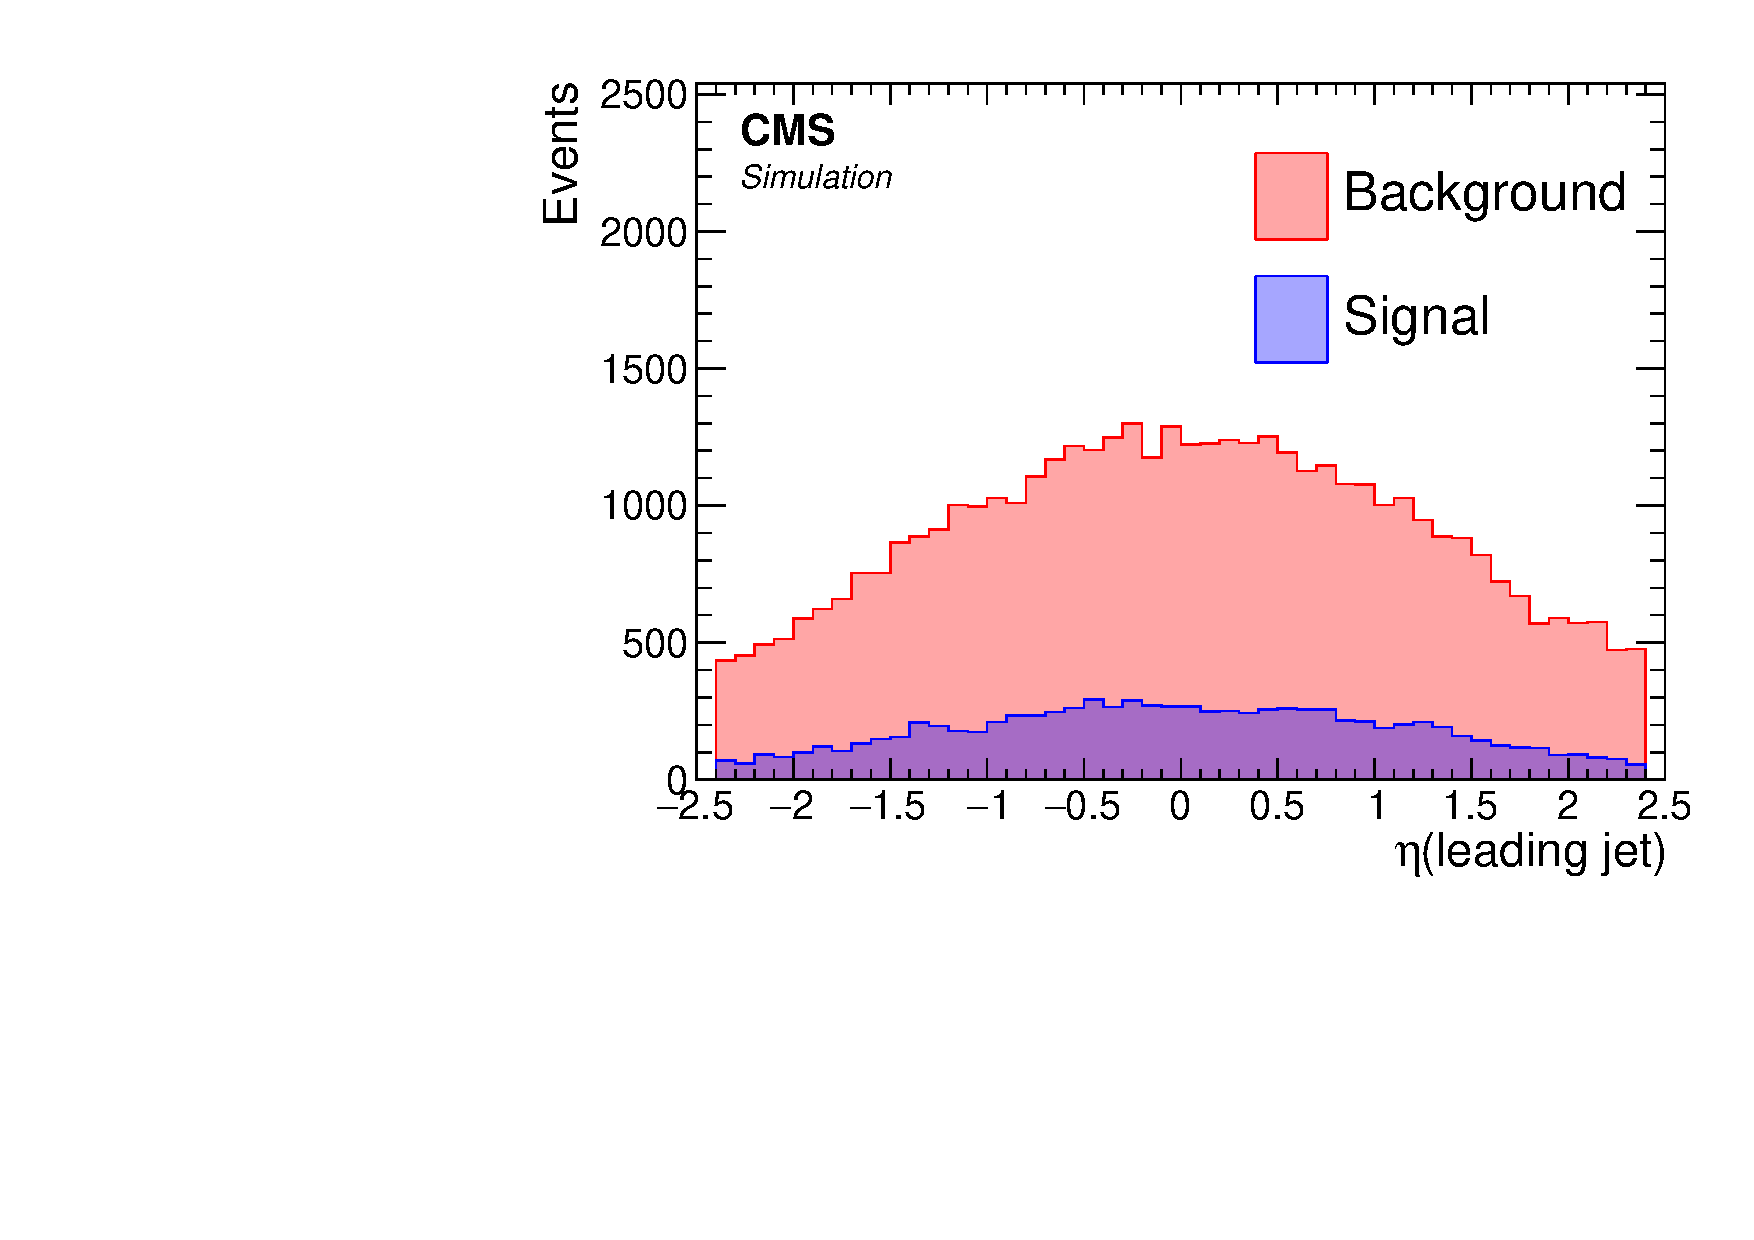
\includegraphics[width=0.32\linewidth]{plots/dilepton_bdt_inputs_muons/none_LeadingJet.Eta__.pdf} \,
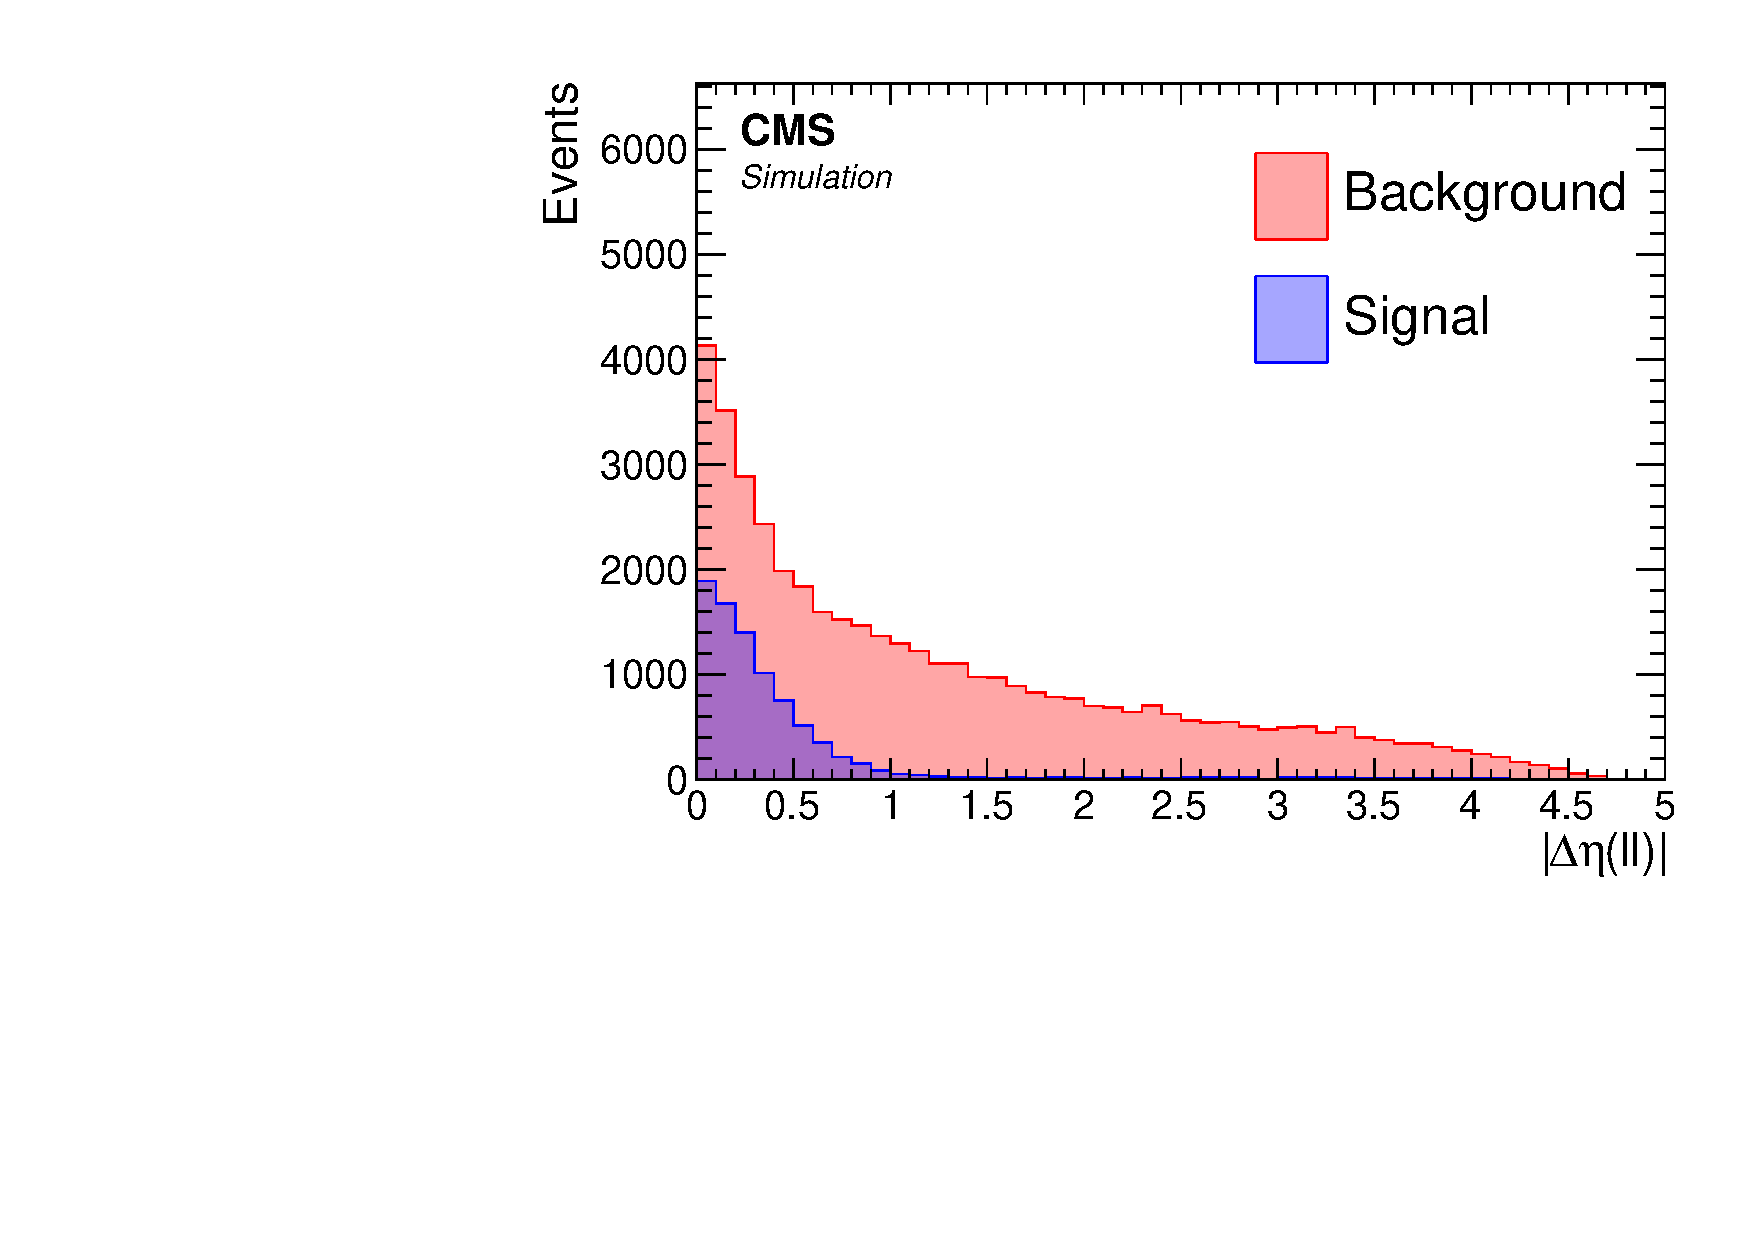
\includegraphics[width=0.32\linewidth]{plots/dilepton_bdt_inputs_muons/none_deltaEtaCorrJetNoMultIso10Dr0.6.pdf}  \,
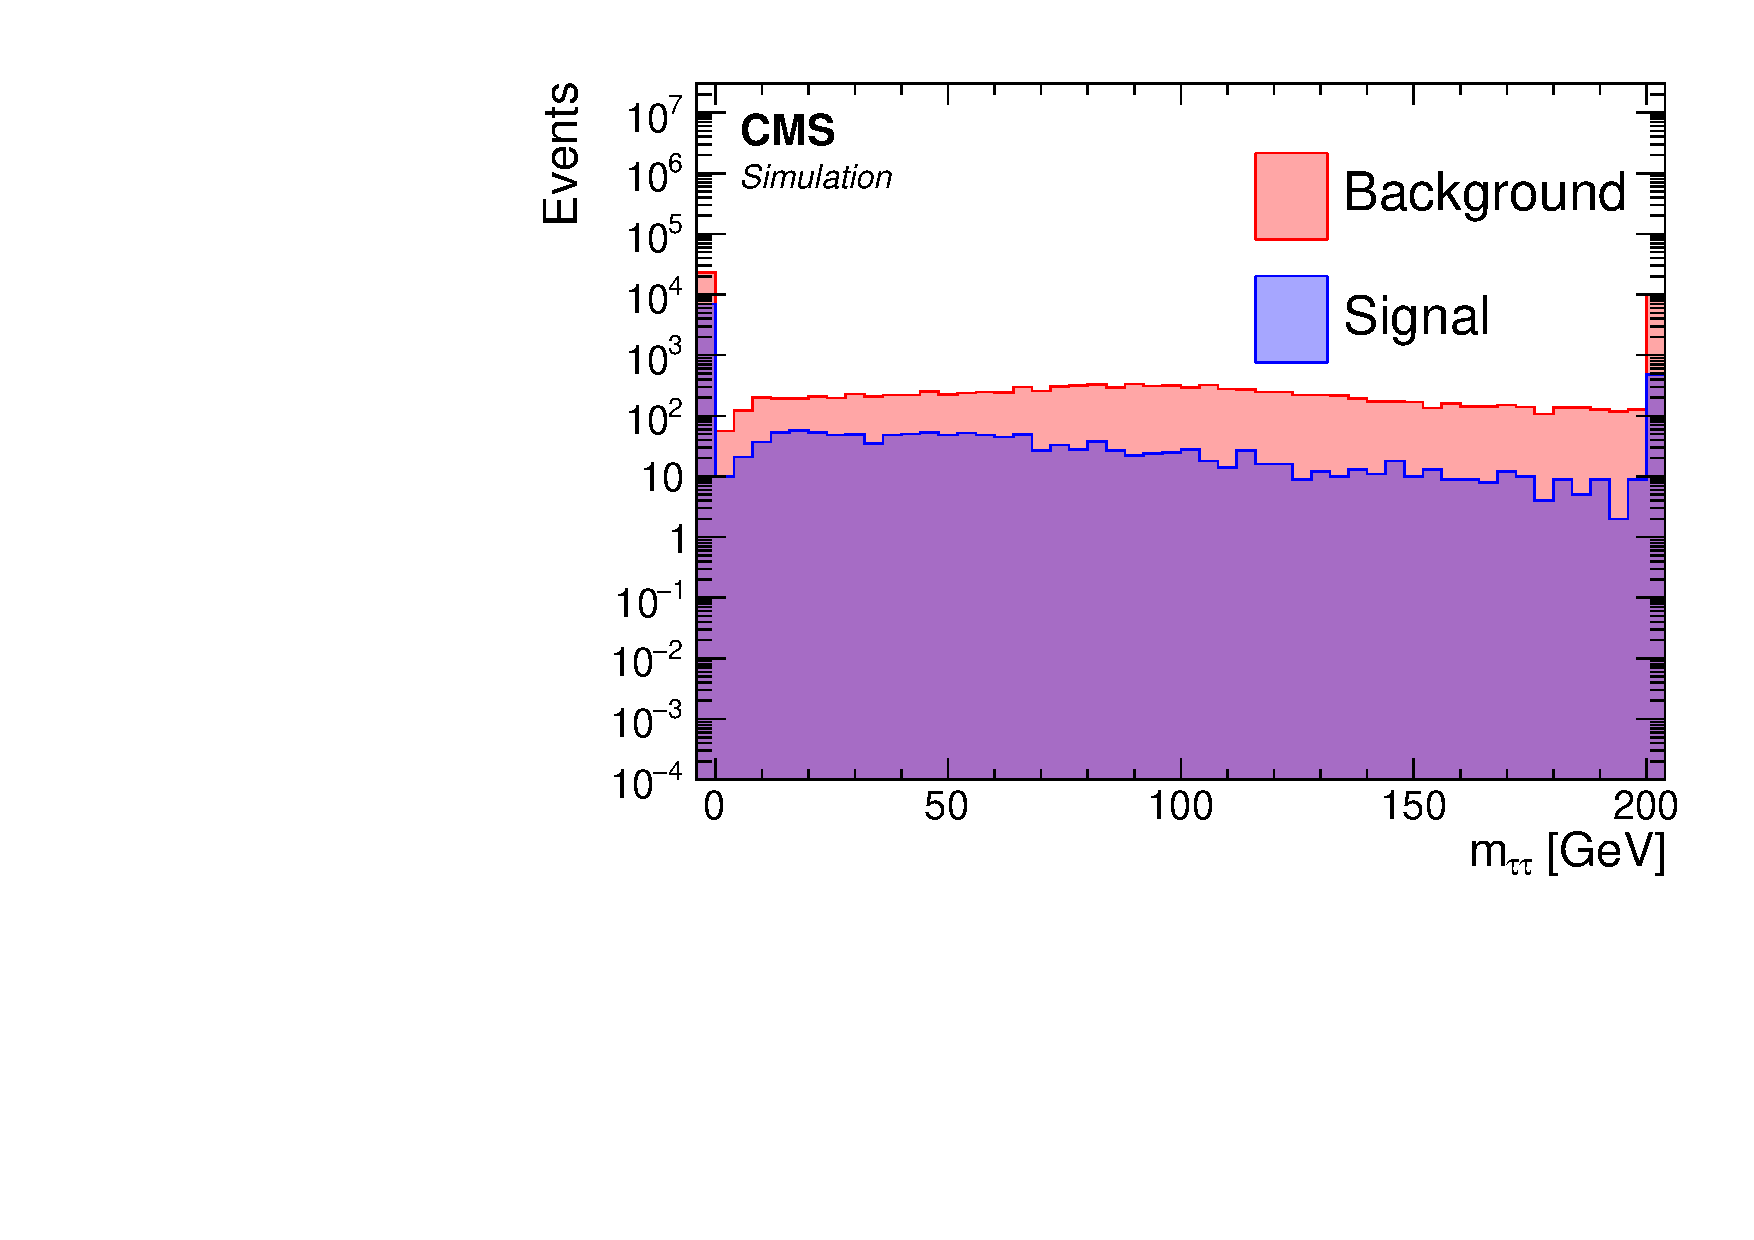
\includegraphics[width=0.32\linewidth]{plots/dilepton_bdt_inputs_muons/none_nmtautauCorrJetNoMultIso10Dr0.6_log.pdf} \\

\caption[dimuon training input distribution]{Dimuon BDT training input variables. The plots are ordered by importance ranking.}
\label{fig:dimuon-input-distributions}
\end{figure}

\clearpage
\subsubsection{Exclusive track category}

The training samples for Phase 0 for the exclusive  category contain 7863 (1750) signal events and 55765 (29135) background events for muons (electrons). For Phase 1, the exclusive category contain 5266 (1332) signal events and 51308 (31149) background events for muons (electrons). The distributions of the testing samples superimposed on the training samples are shown in Figure~\ref{fig:event-bdt-ex-track-output}. The ROC curves are seen in Figure~\ref{fig:event-bdt-ex-track-roc}. No over training is observed.

\begin{figure}[!htb]
\centering
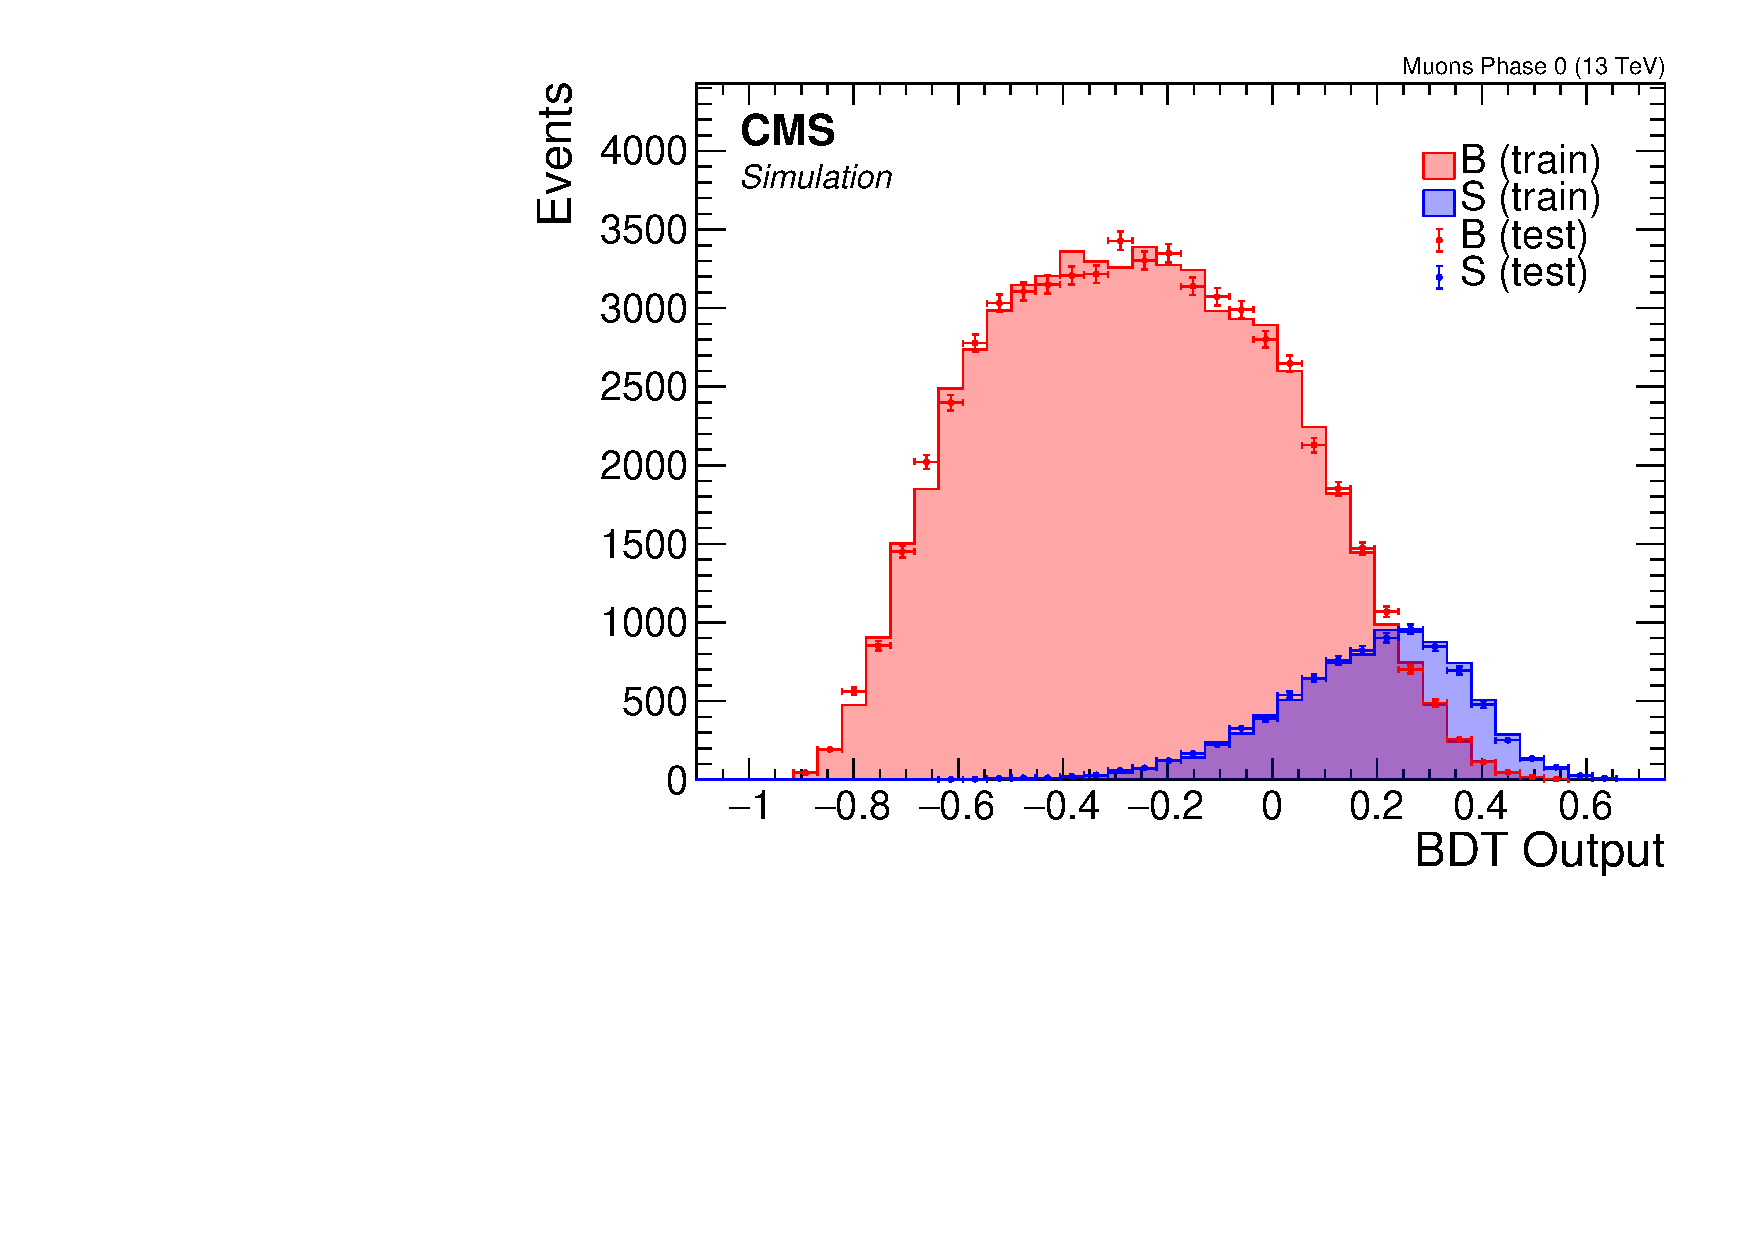
\includegraphics[width=0.48\linewidth]{plots/extrack_bdt/overtraining_Event_Ex_Track_Muons_Phase_0.pdf} \,
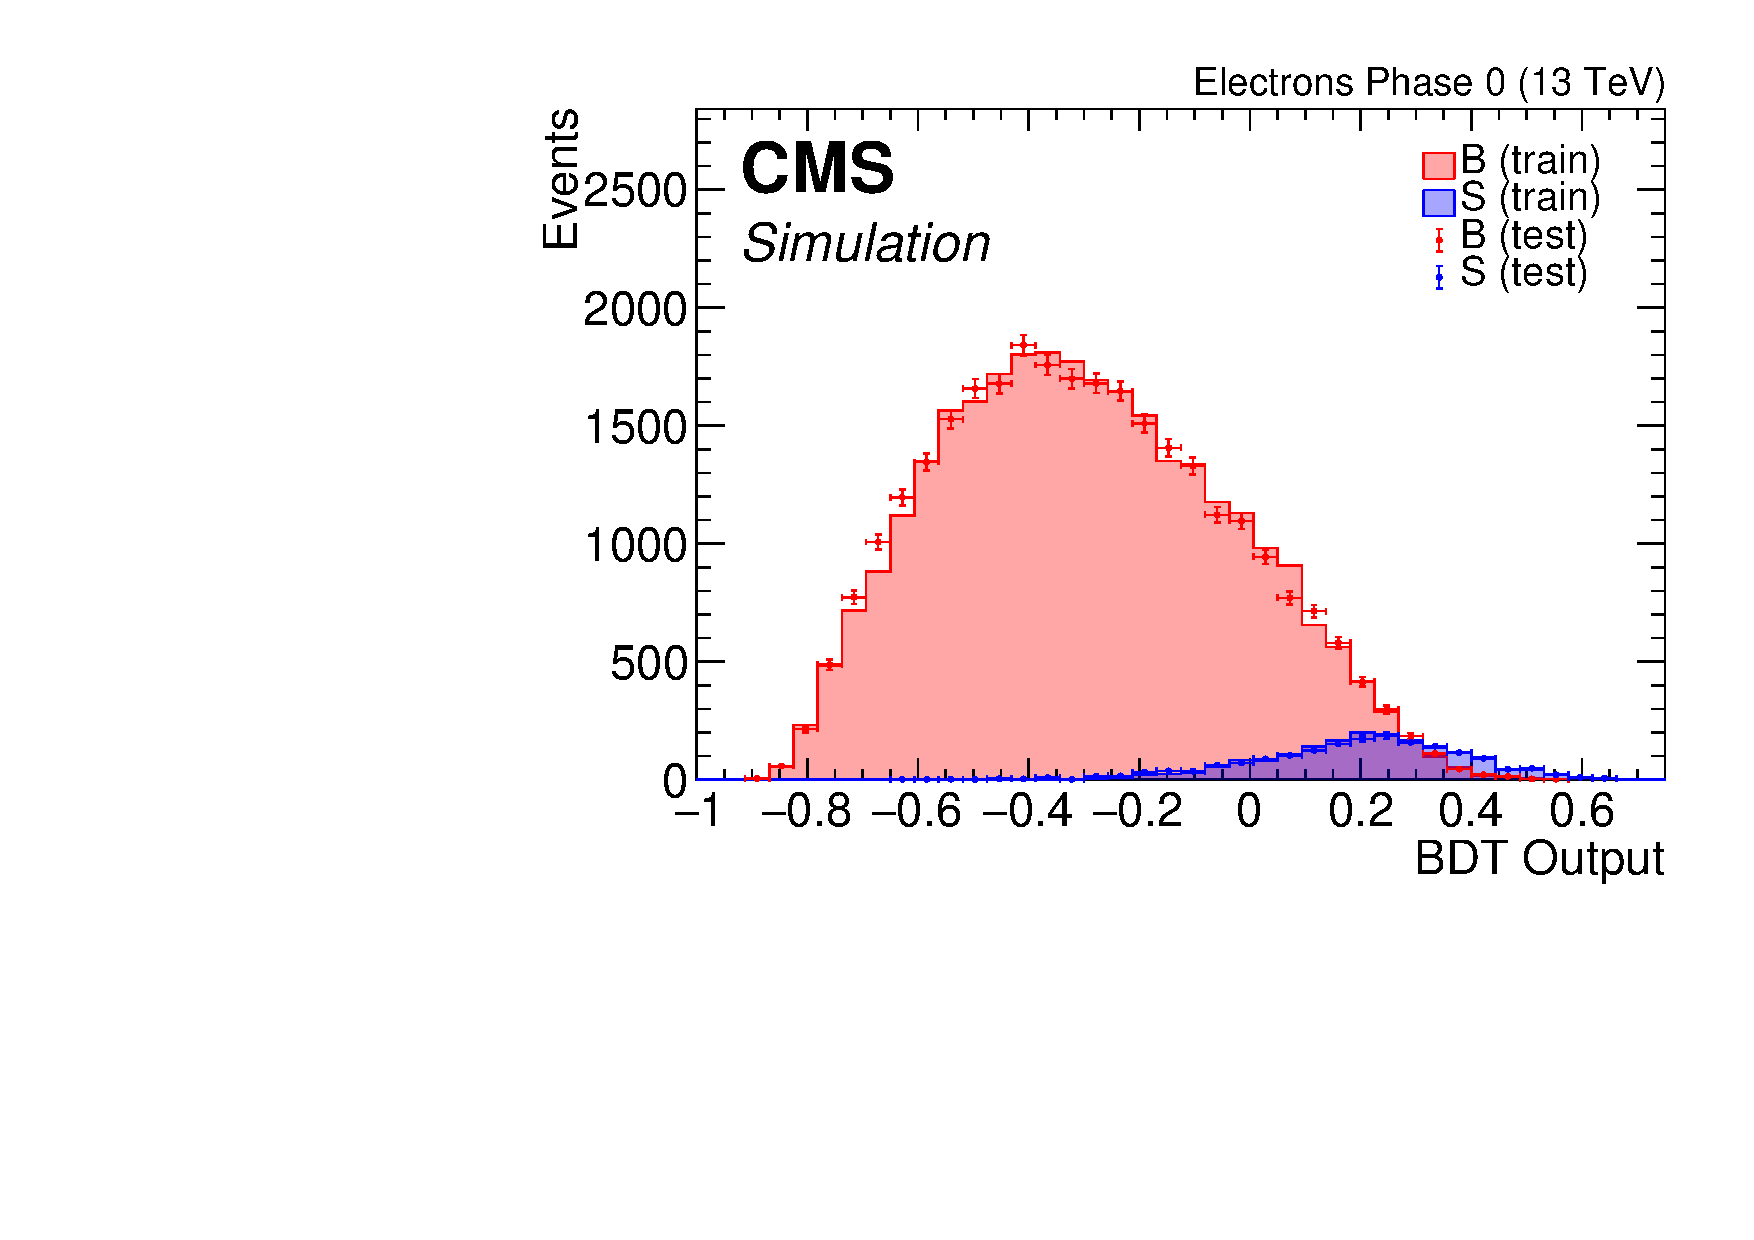
\includegraphics[width=0.48\linewidth]{plots/extrack_bdt/overtraining_Event_Ex_Track_Electrons_Phase_0.pdf} \\

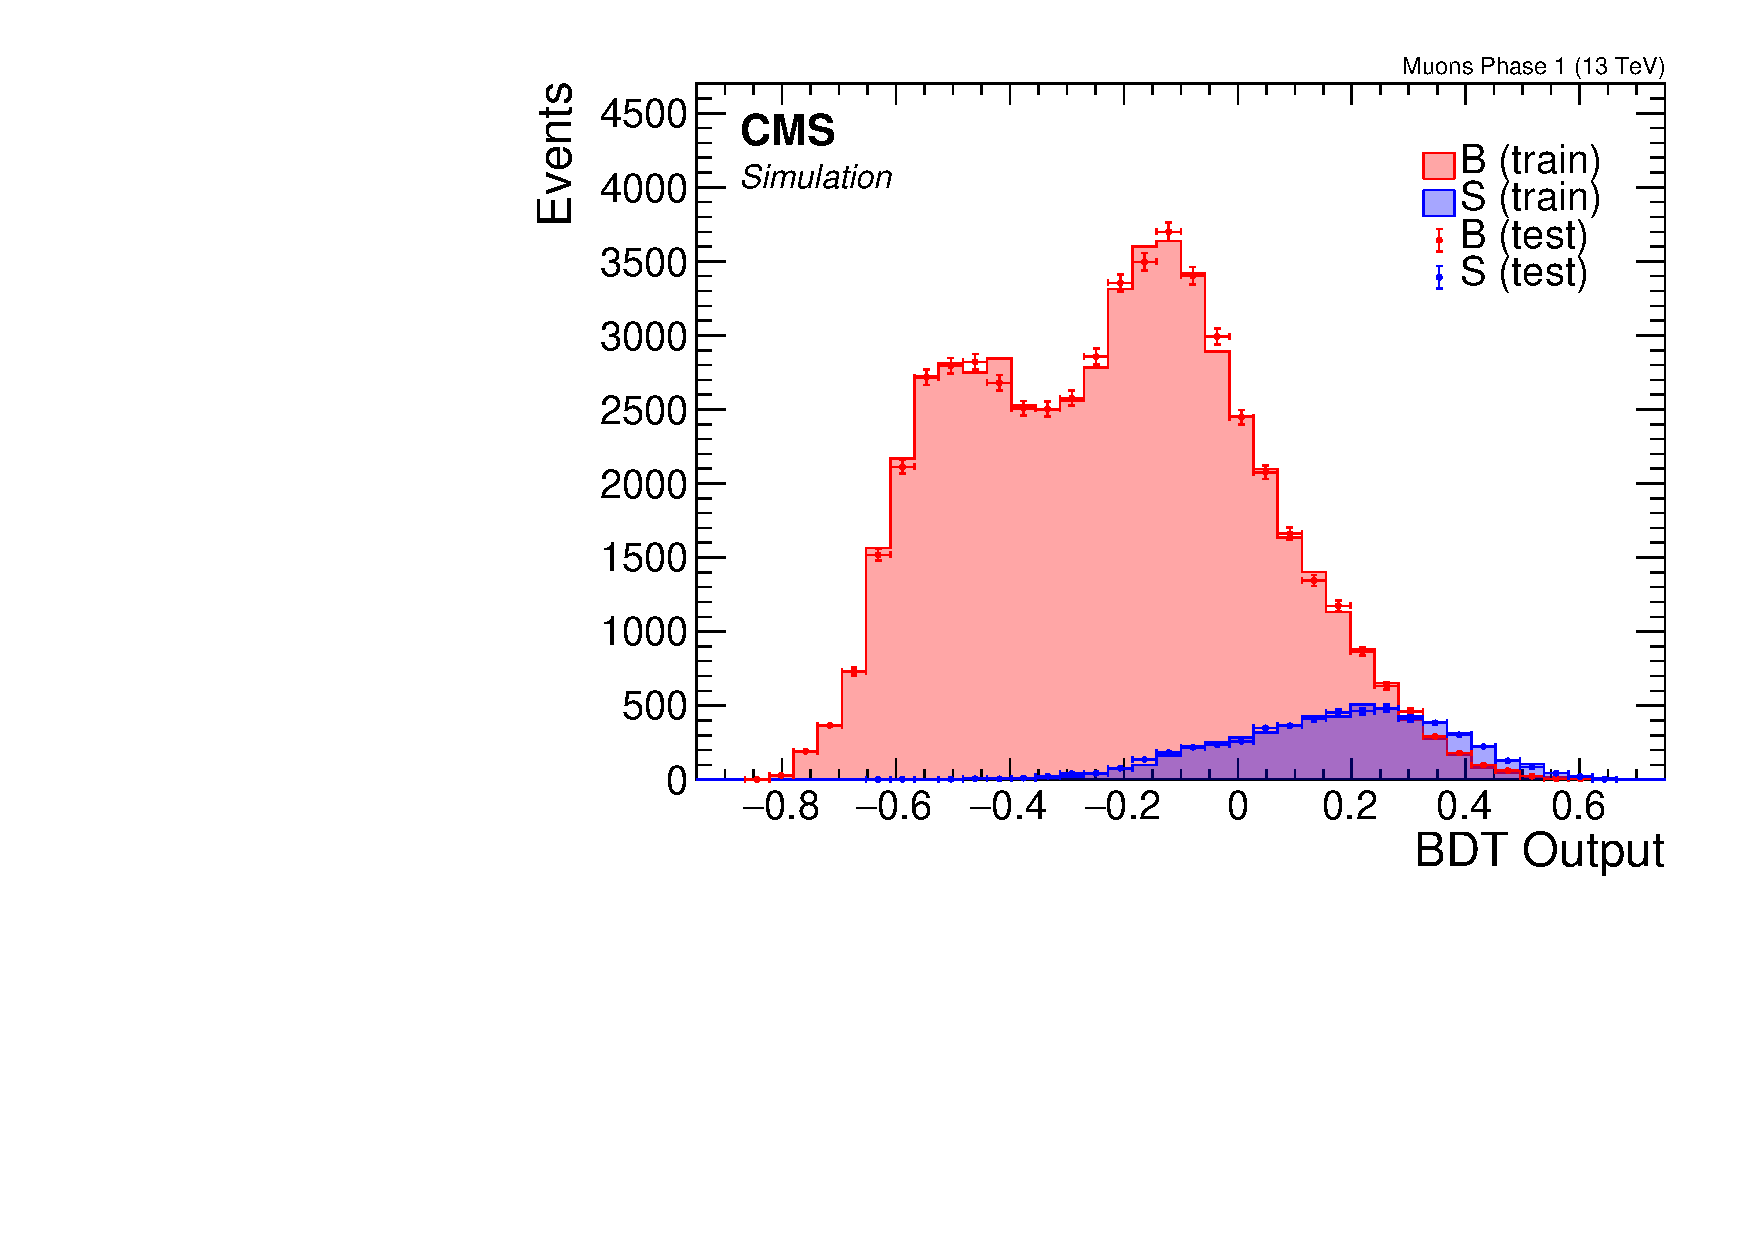
\includegraphics[width=0.48\linewidth]{plots/extrack_bdt/overtraining_Event_Ex_Track_Muons_Phase_1.pdf} \,
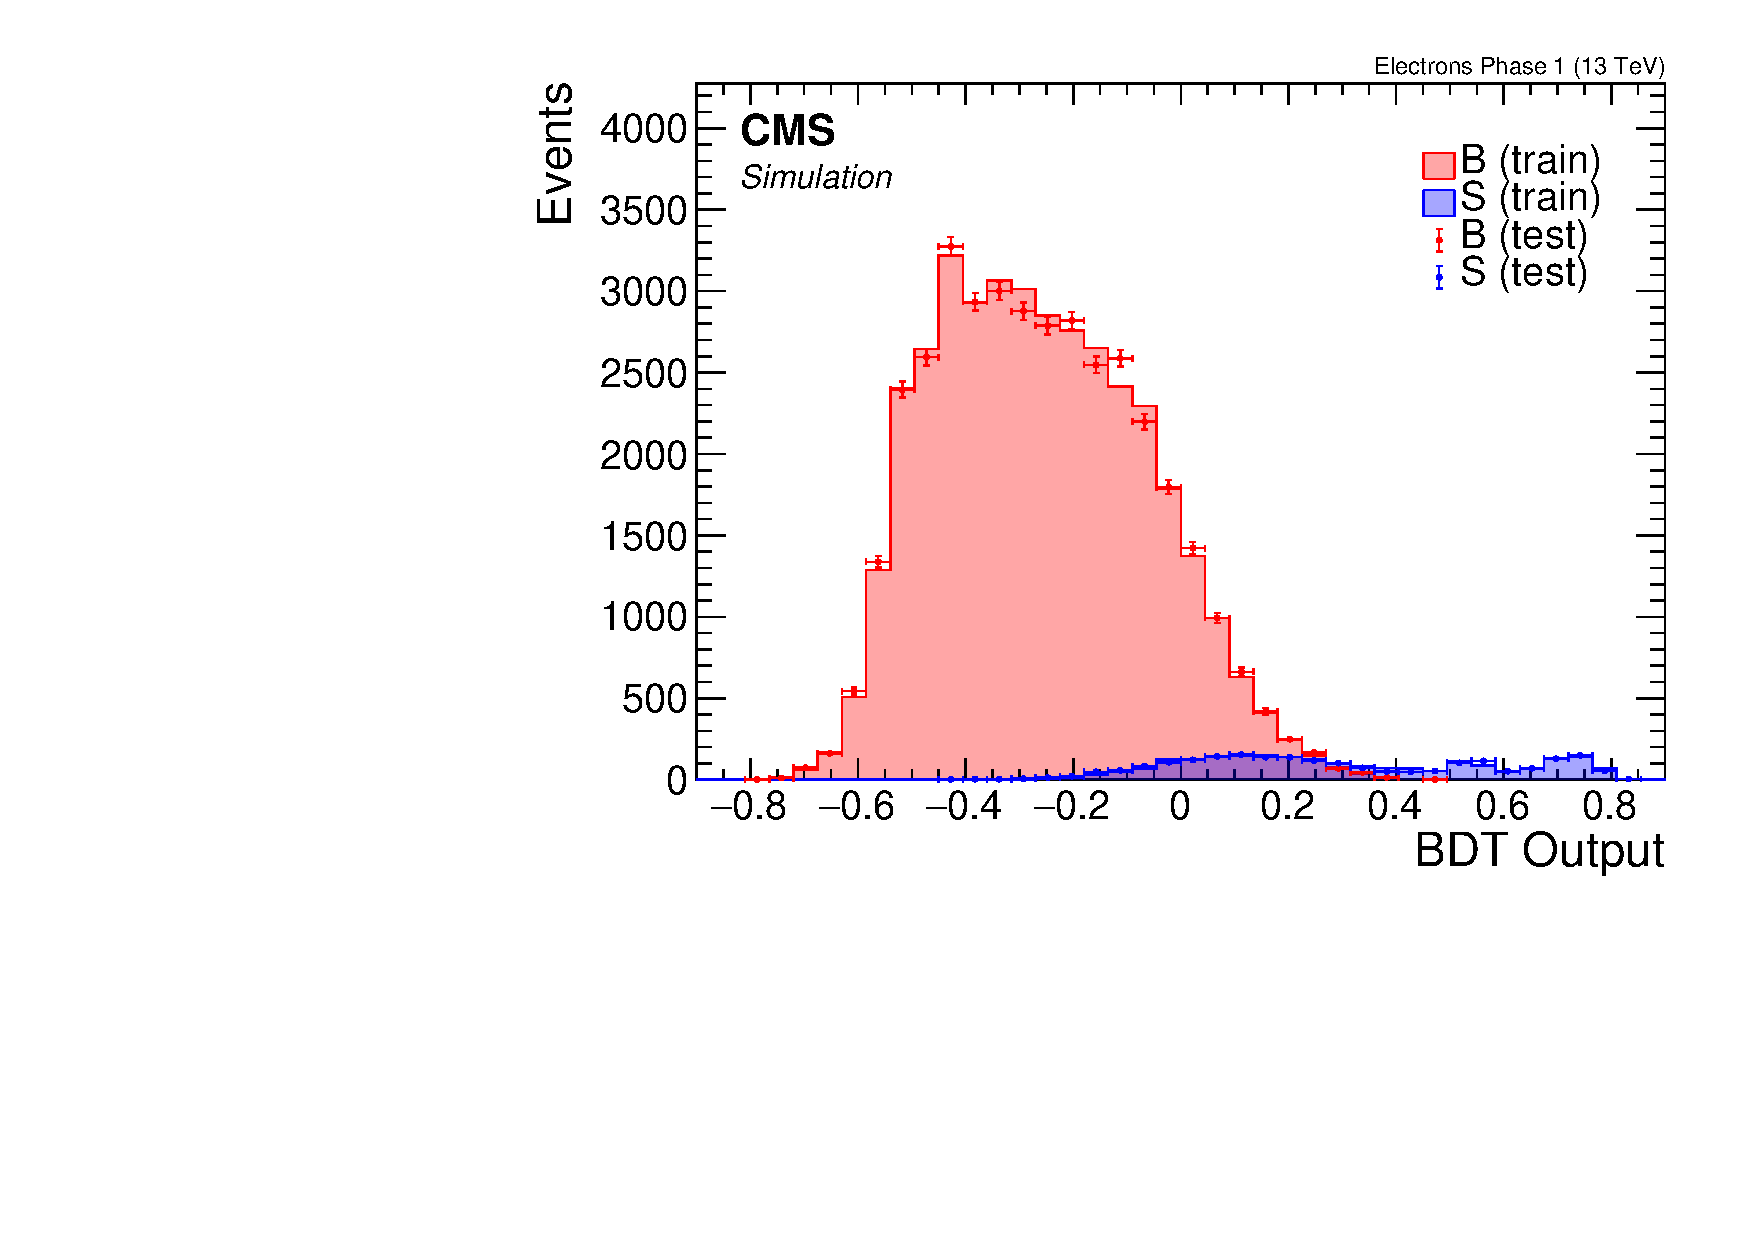
\includegraphics[width=0.48\linewidth]{plots/extrack_bdt/overtraining_Event_Ex_Track_Electrons_Phase_1.pdf} \\

\caption[Exclusive track category BDT outputs]{Exclusive track category BDT output in Phase 0 (top) and Phase 1 (bottom) for muons (left) and electrons (right).}
\label{fig:event-bdt-ex-track-output}
\end{figure}

\begin{figure}[!htb]
\centering
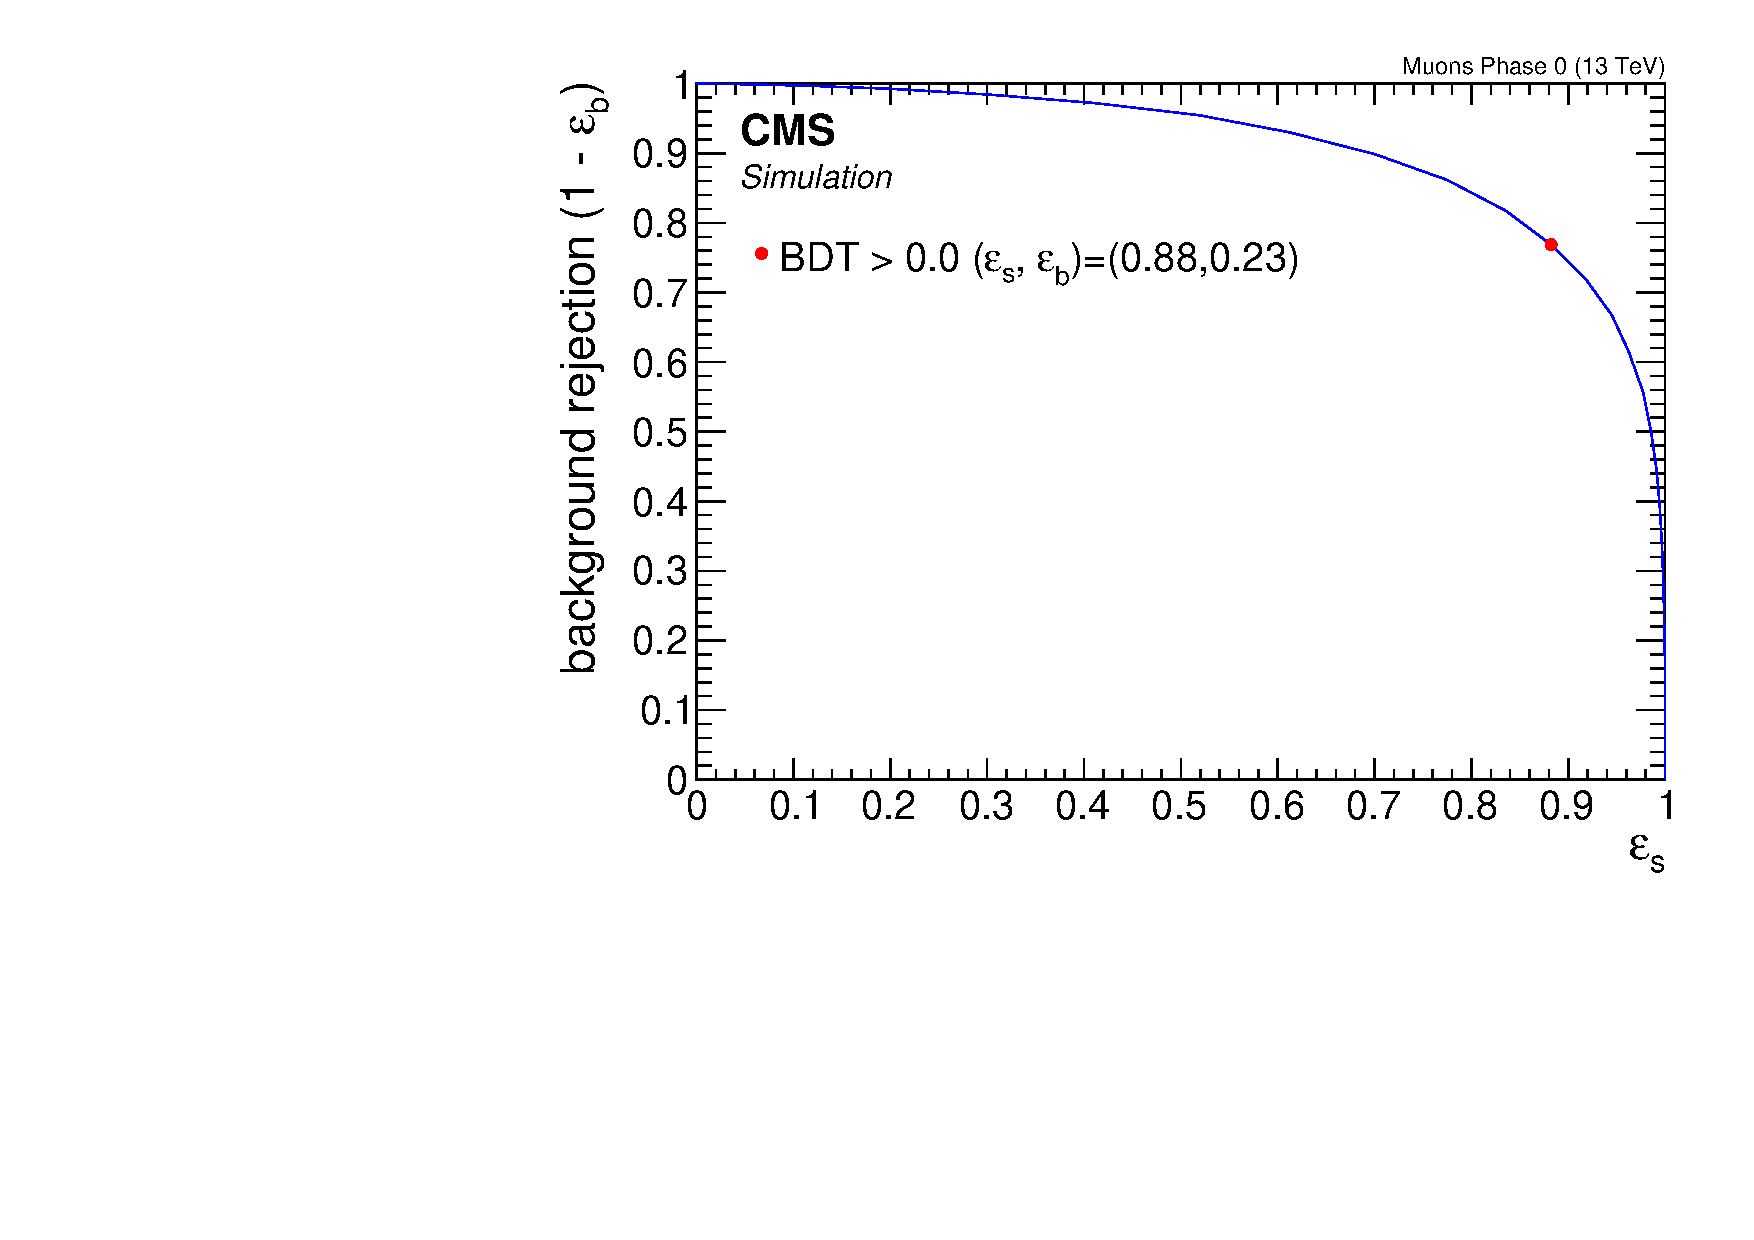
\includegraphics[width=0.48\linewidth]{plots/extrack_bdt/roc_Event_Ex_Track_Muons_Phase_0.pdf} \,
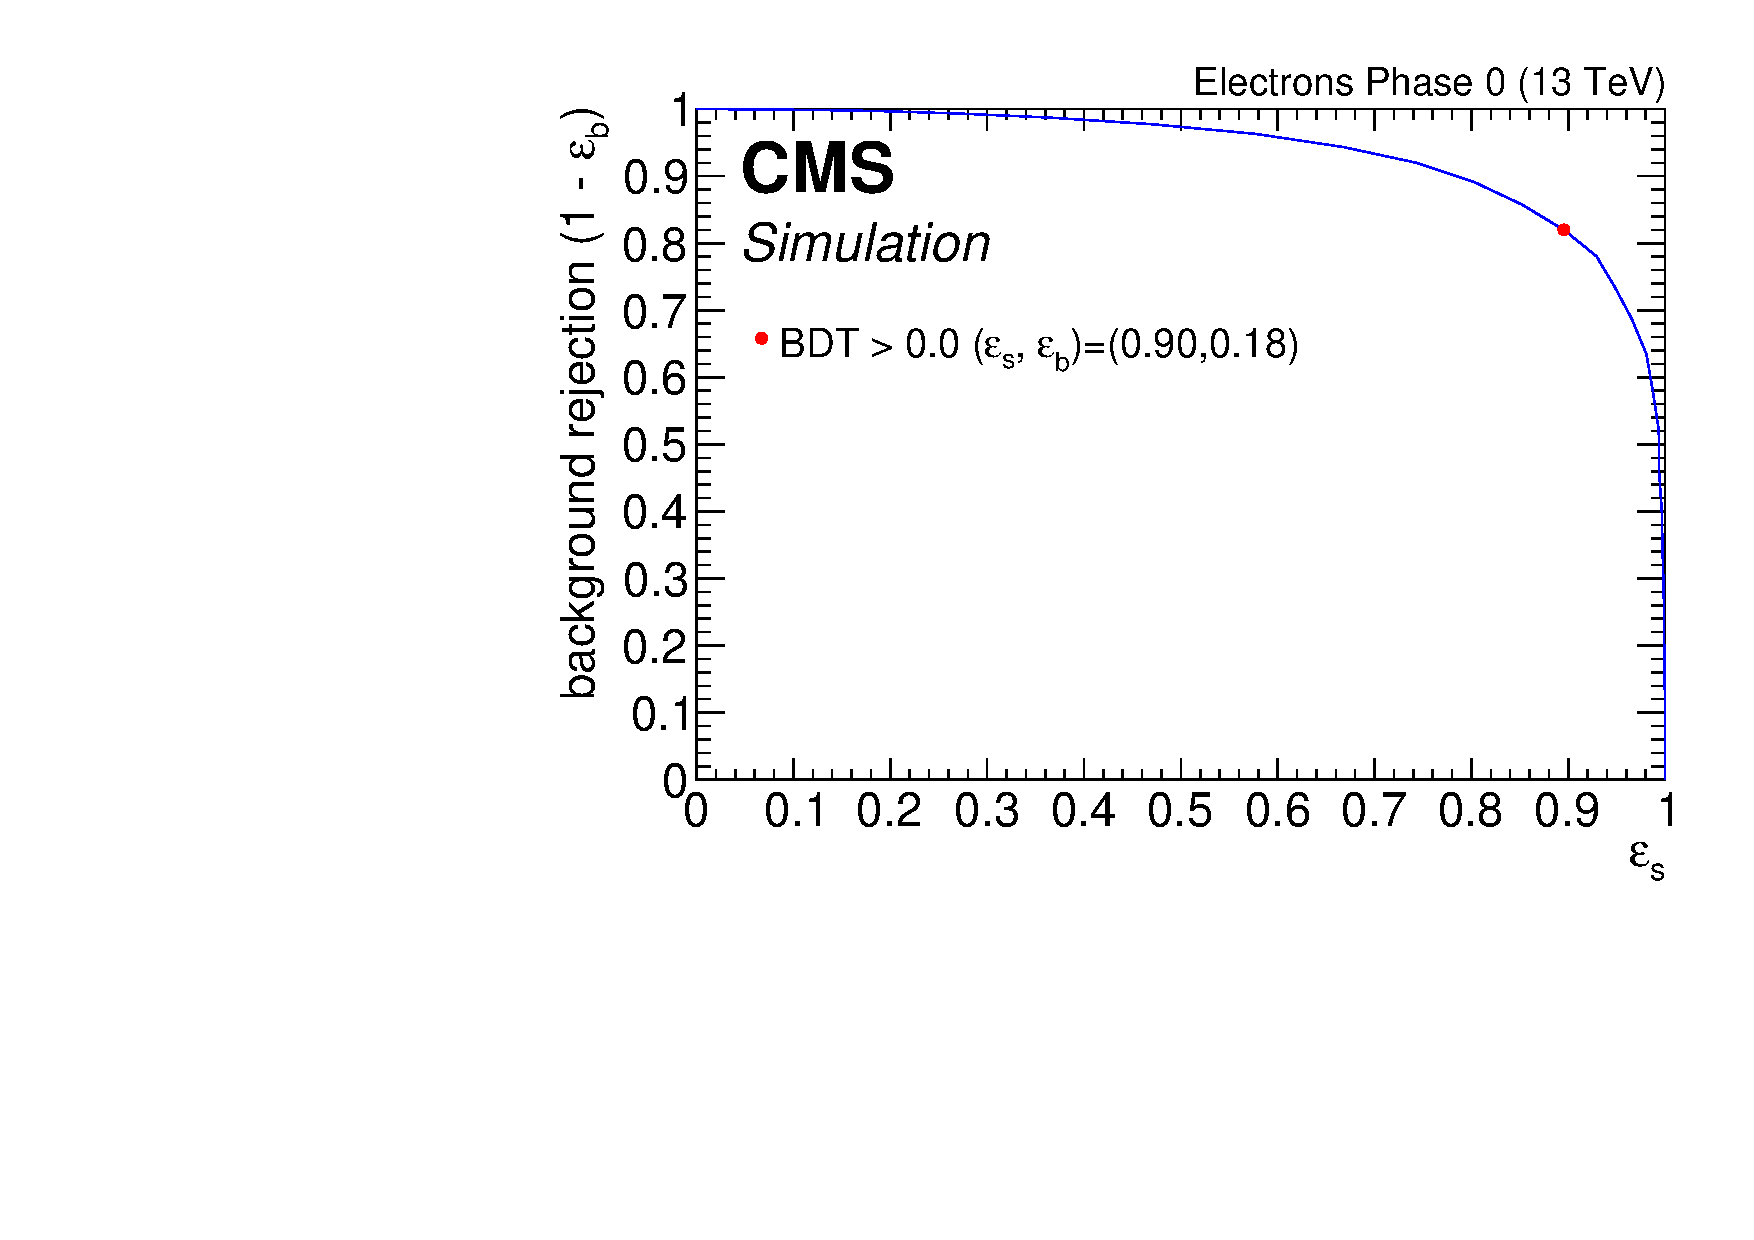
\includegraphics[width=0.48\linewidth]{plots/extrack_bdt/roc_Event_Ex_Track_Electrons_Phase_0.pdf} \\

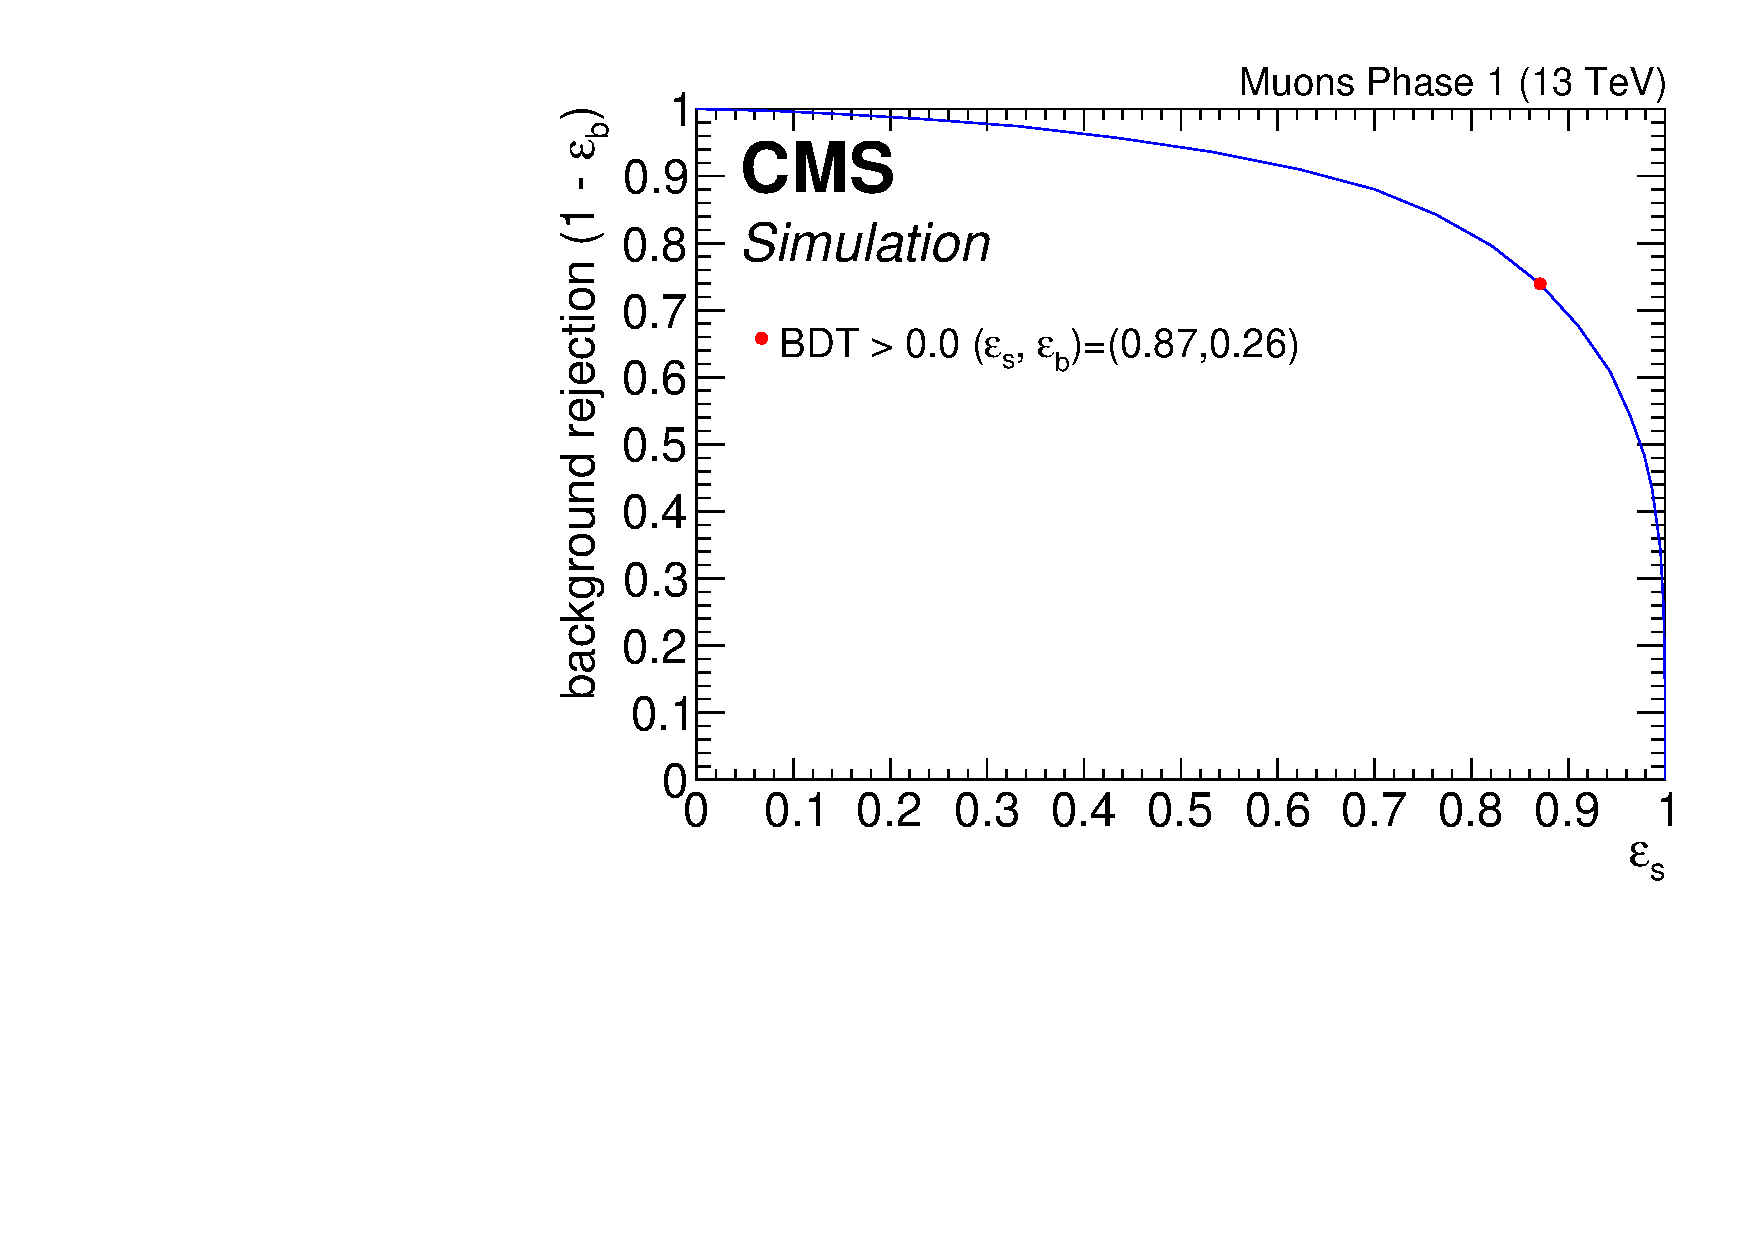
\includegraphics[width=0.48\linewidth]{plots/extrack_bdt/roc_Event_Ex_Track_Muons_Phase_1.pdf} \,
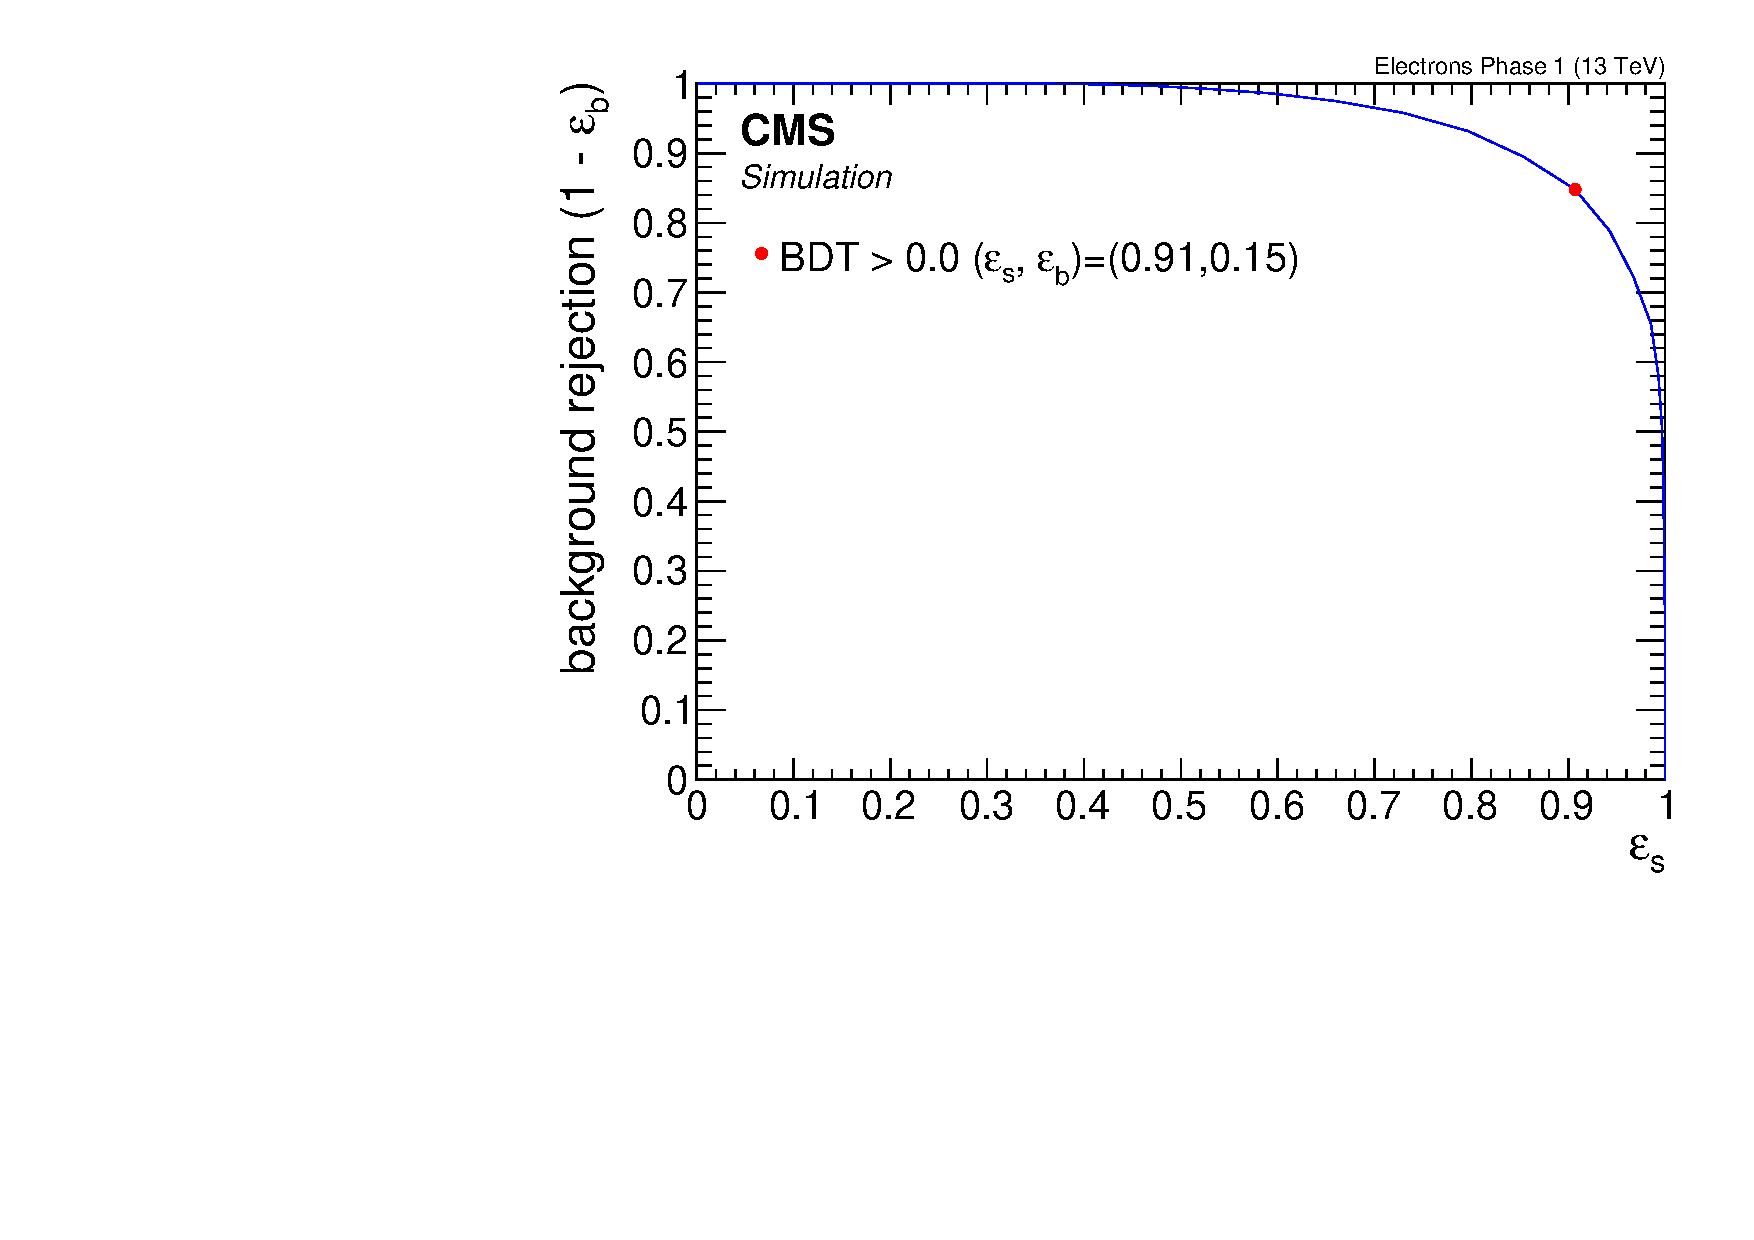
\includegraphics[width=0.48\linewidth]{plots/extrack_bdt/roc_Event_Ex_Track_Electrons_Phase_1.pdf} \\

\caption[Exclusive track category ROC curve]{Exclusive track category ROC curves in Phase 0 (top) and Phase 1 (bottom) for muons (left) and electrons (right)}
\label{fig:event-bdt-ex-track-roc}
\end{figure}

The training uses 18 different variables listed in Table~\ref{tab:extrack-bdt-variables} in decreasing order of importance ranking. Since the ranking is slightly different in the four trainings, the order in the case of the muons of phase 1 is chosen to be listed here. The fully identified lepton is denoted as $\ell$ and the non-identified lepton track as $t$.

\begin{table}[!htb]
	\centering
	\label{tab:extrack-bdt-variables}
		\caption{Exclusive track BDT input variables}
		%\vspace{1mm}
			\begin{tabular}{cll} \hline
			Rank & Variable & Description \\ \hline
			1 & $\pt(\ell)$ & lepton \pt\\
			2 & \HT & \\
			3 & \mht & \\
			4 & $\mindphimhtjets$ & \\
			5 & $\pt(\text{leading jet})$ & \\
			6 & $\njets$ & Number of jets \\					7 & track BDT output & \\
			8 & $\eta(t)$ & \\
			9 & $\pt(t)$ & track \pt\\
			10 & $\eta(\text{leading jet})$ & \\				11 & $\mll$ & invariant mass \\
			12 & $\eta(\ell)$ & \\
			13 & $m_T(\ell)$ & lepton transverse mass\\			
			14 & $\DR\left(\ell, t\right)$ & \\
			15 & $\phi(\ell)$ & \\
			16 & $\phi(t)$ & \\
			17 & $\abs{\Delta\phi\left(\ell,t \right)}$ & \\			
			18 & $\abs{\Delta \eta \left(\ell, t\right) }$ & \\			
			\hline
			\end{tabular}
\end{table}

Distributions of the input variables to the \gls{bdt} training can be seen in Figure~\ref{fig:extrack-input-distributions}. As mentioned before, the signal is taken from a pool of a range of model points, and events are not weighted to any luminosity or cross section in order to avoid over training. In the following sections we fully weighted distributions will be shown in order to asses the performance of the training for different model points and to understand the different components of the standard model background and how to estimate it properly.

\begin{figure}[!htb]
\centering
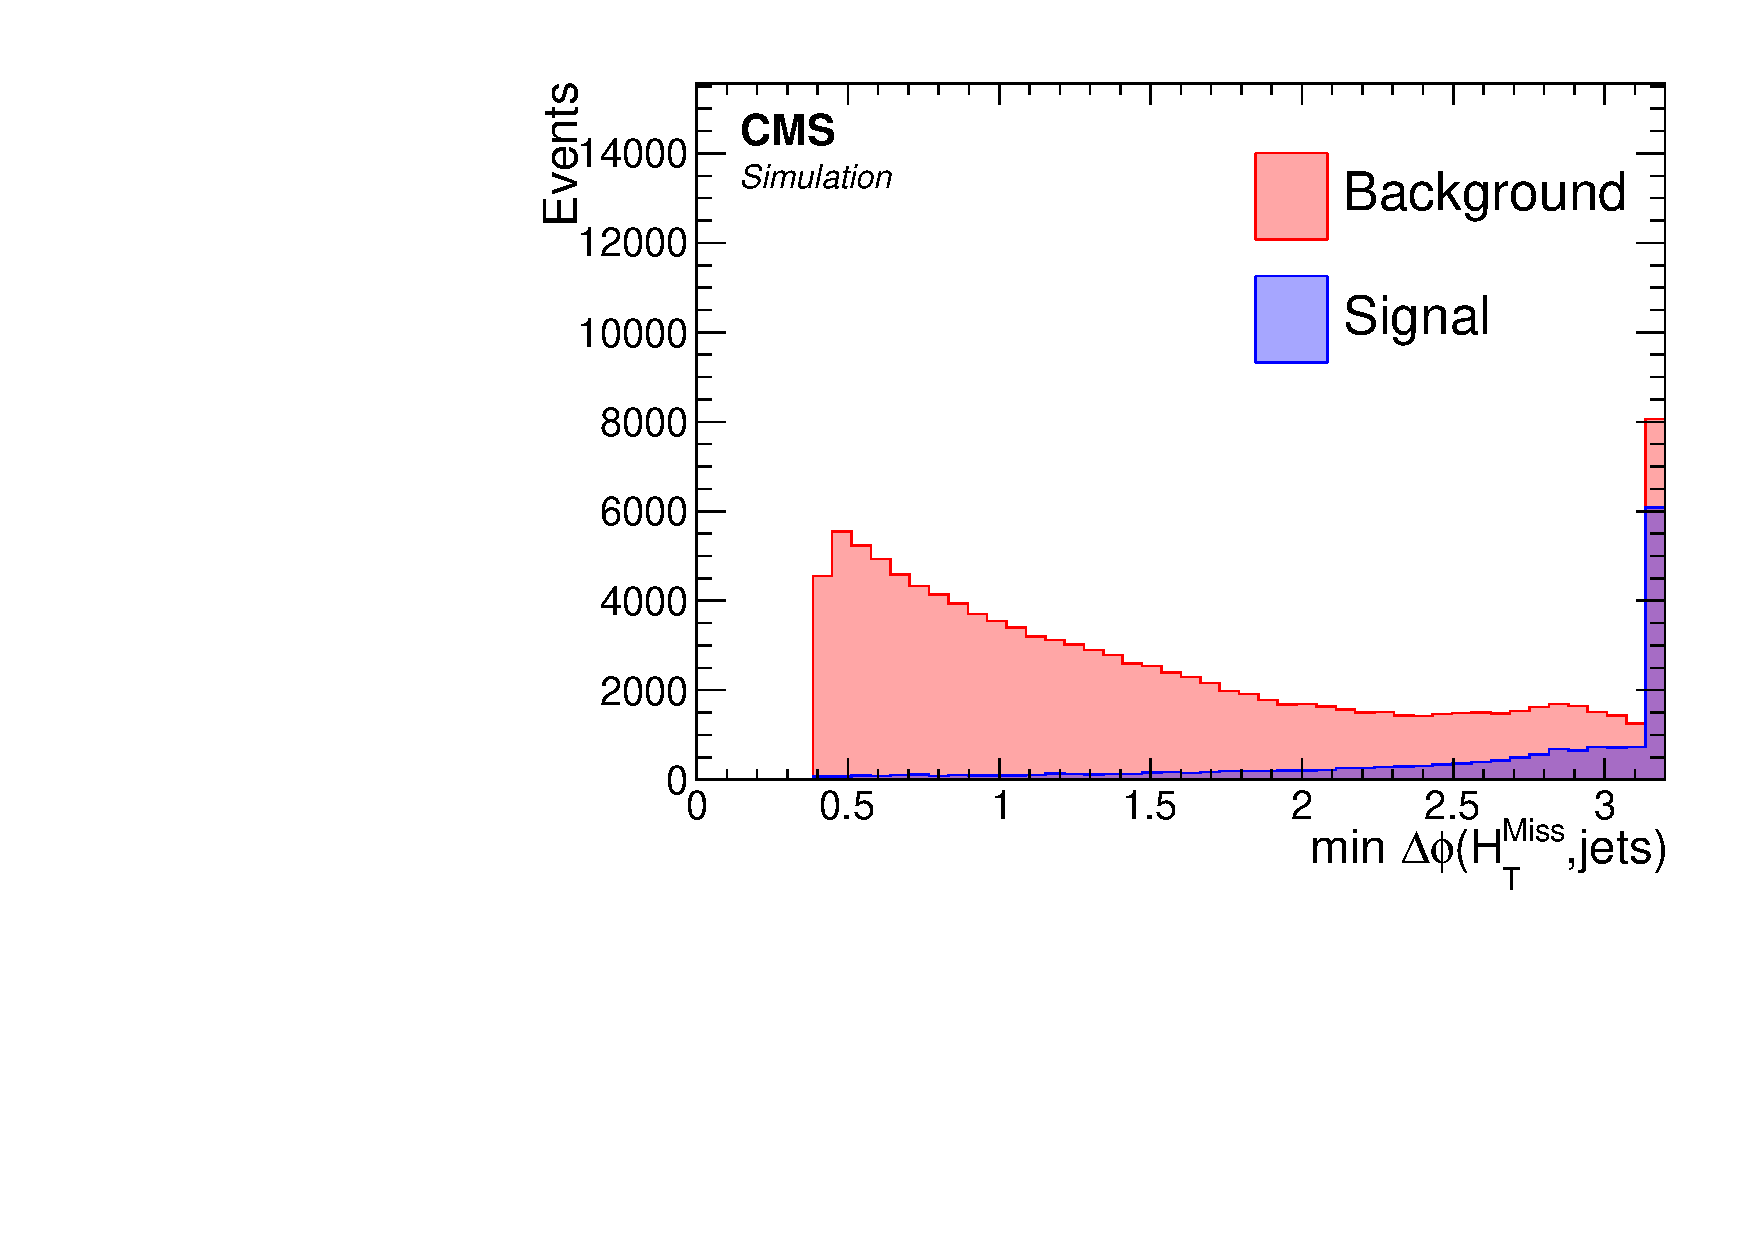
\includegraphics[width=0.32\linewidth]{plots/extrack_bdt_inputs_muons/none_MinDeltaPhiMhtJets.pdf} \,
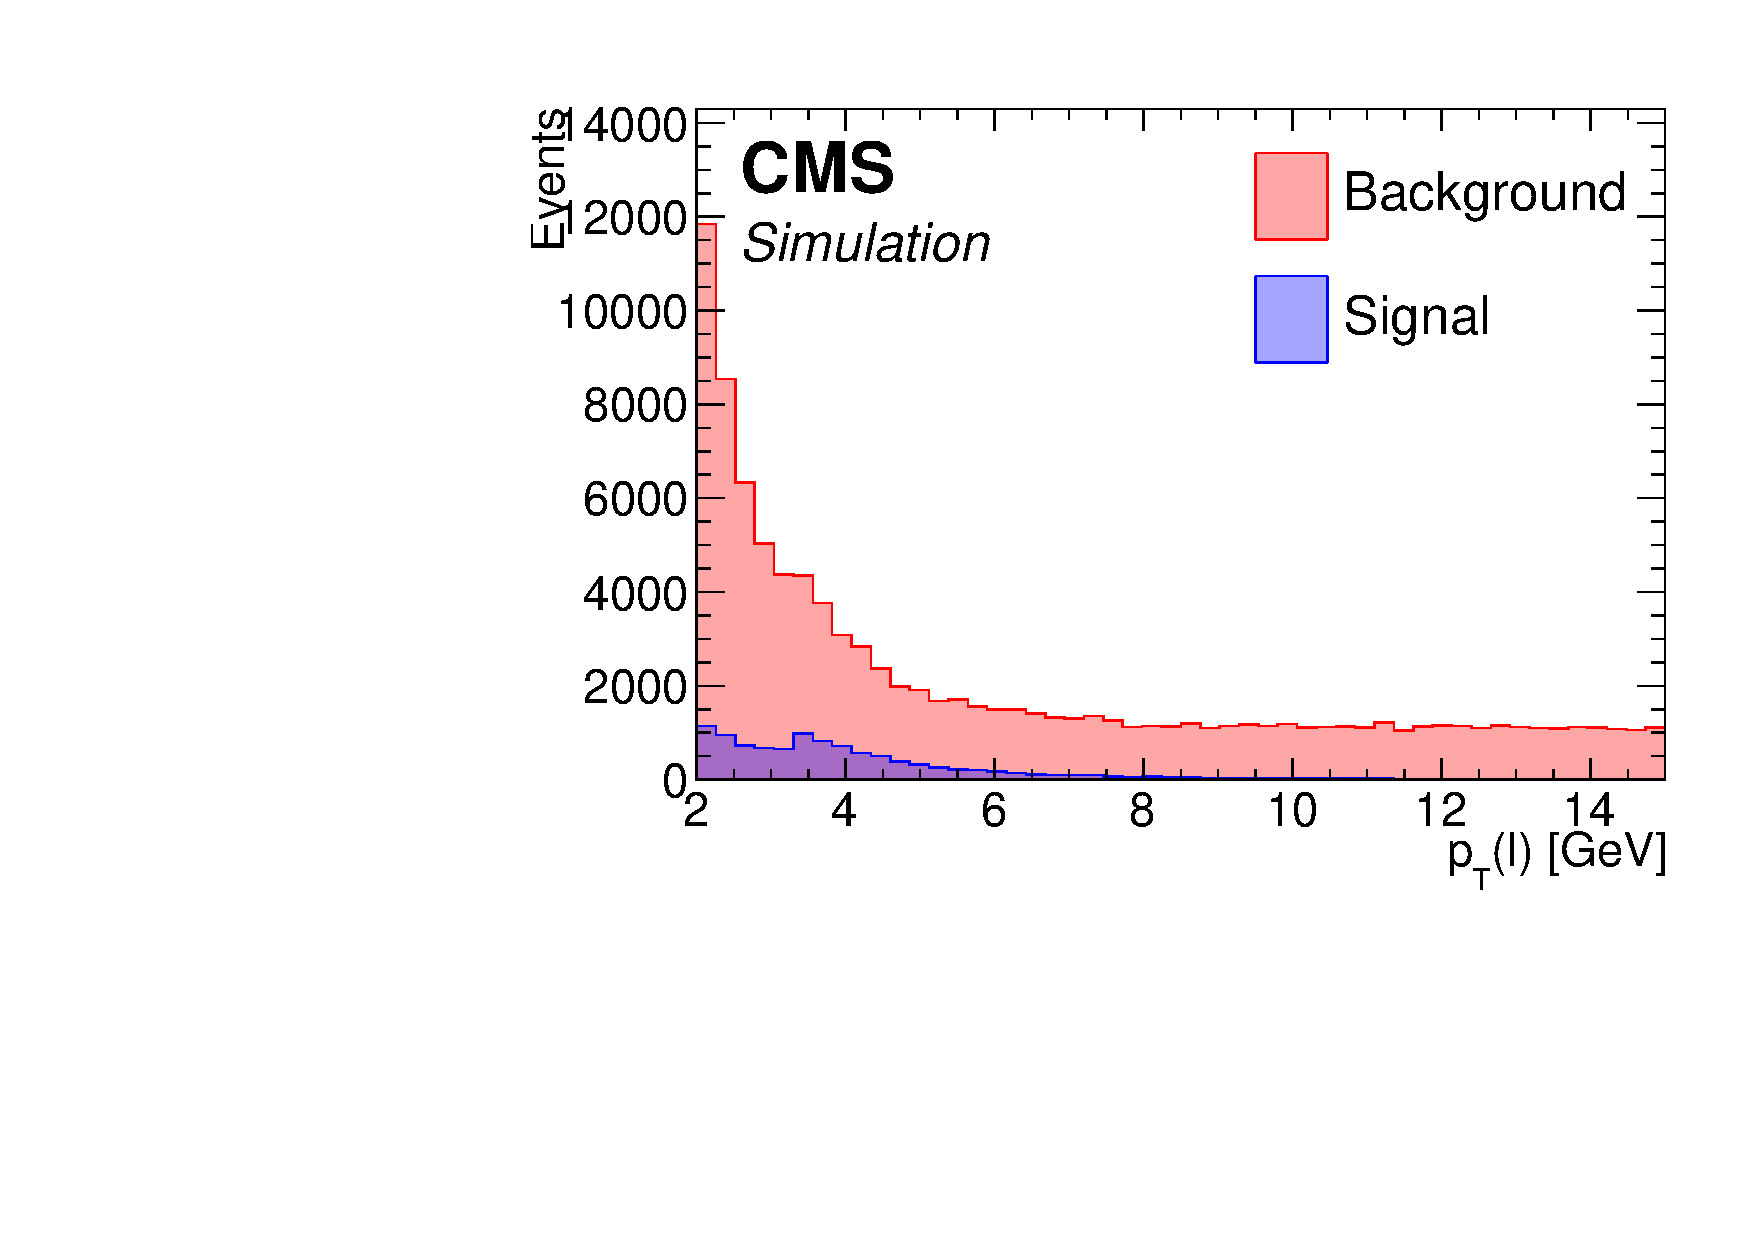
\includegraphics[width=0.32\linewidth]{plots/extrack_bdt_inputs_muons/none_leptonCorrJetNoMultIso10Dr0.6.Pt__.pdf} \,
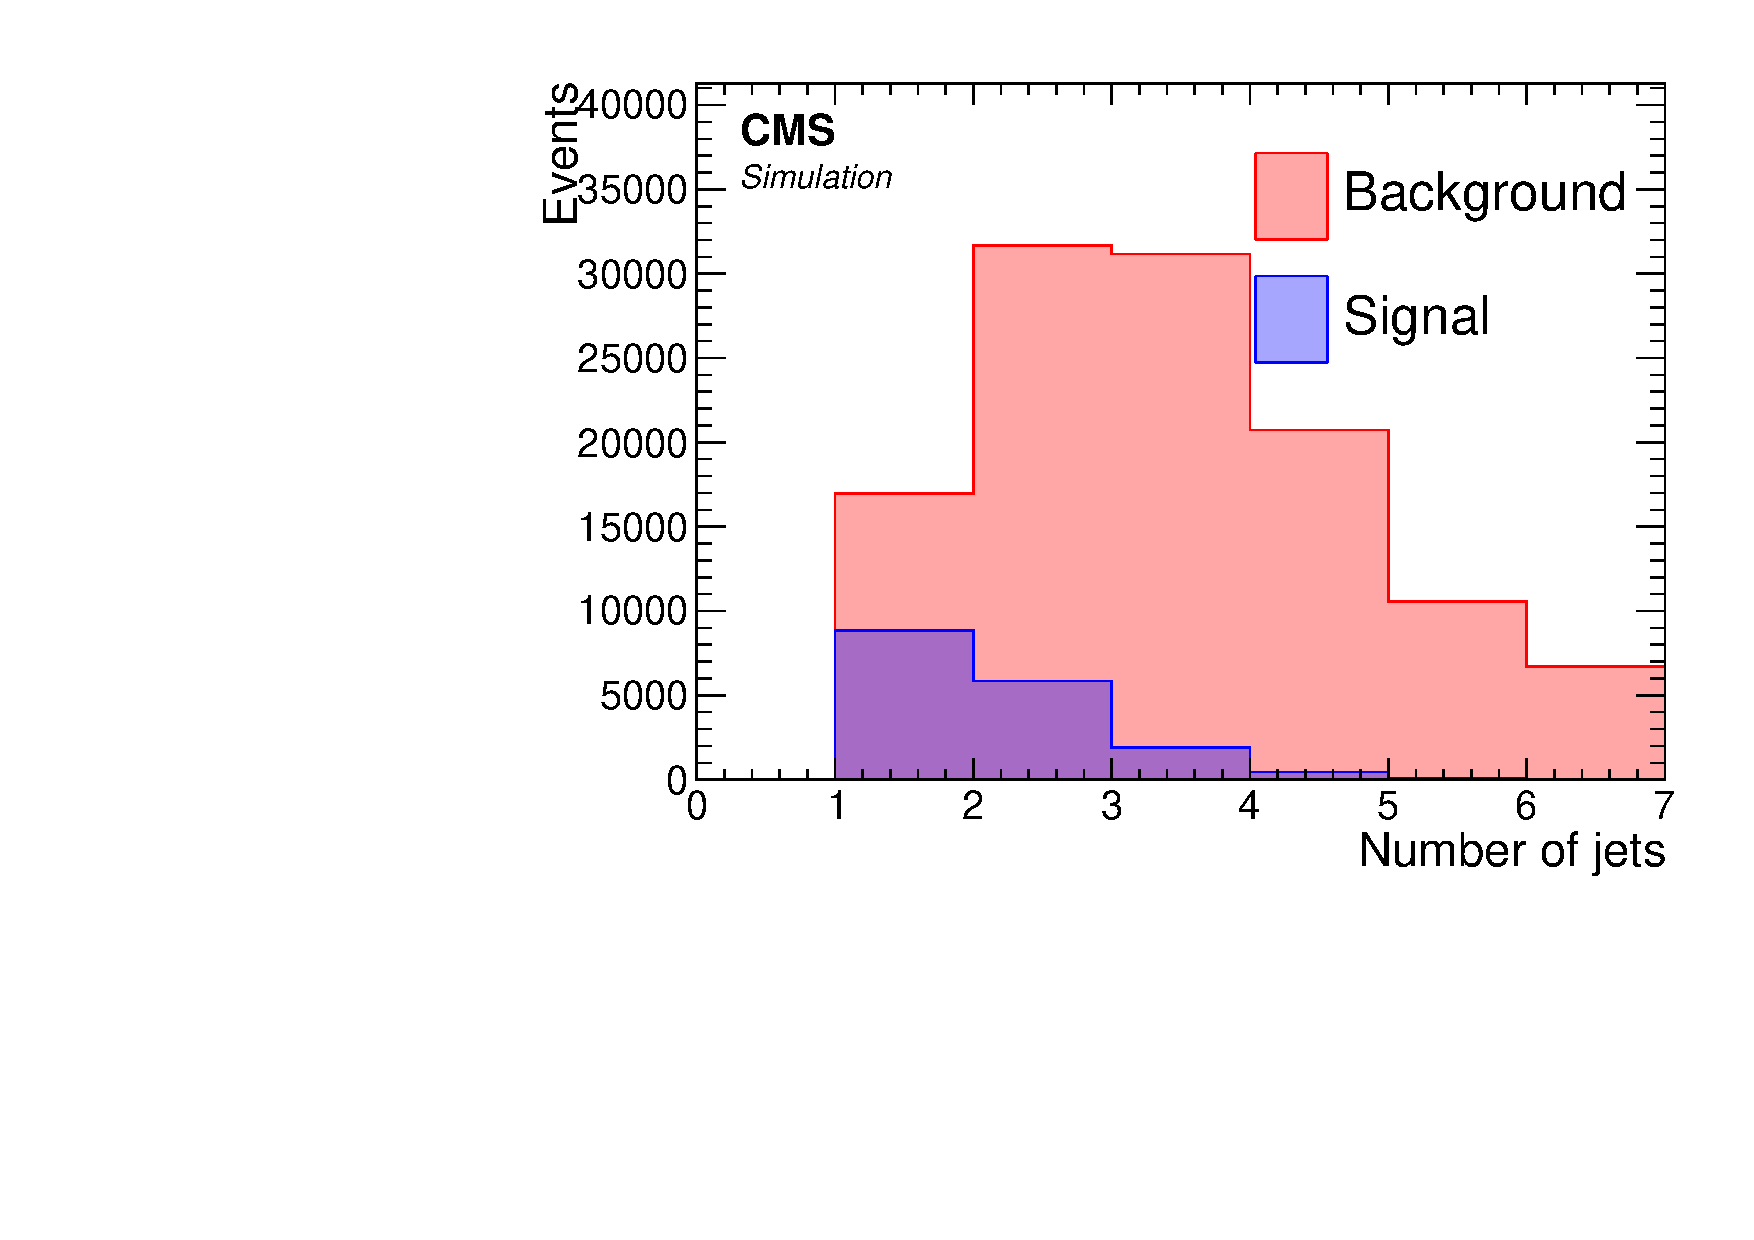
\includegraphics[width=0.32\linewidth]{plots/extrack_bdt_inputs_muons/none_NJets.pdf}   \\
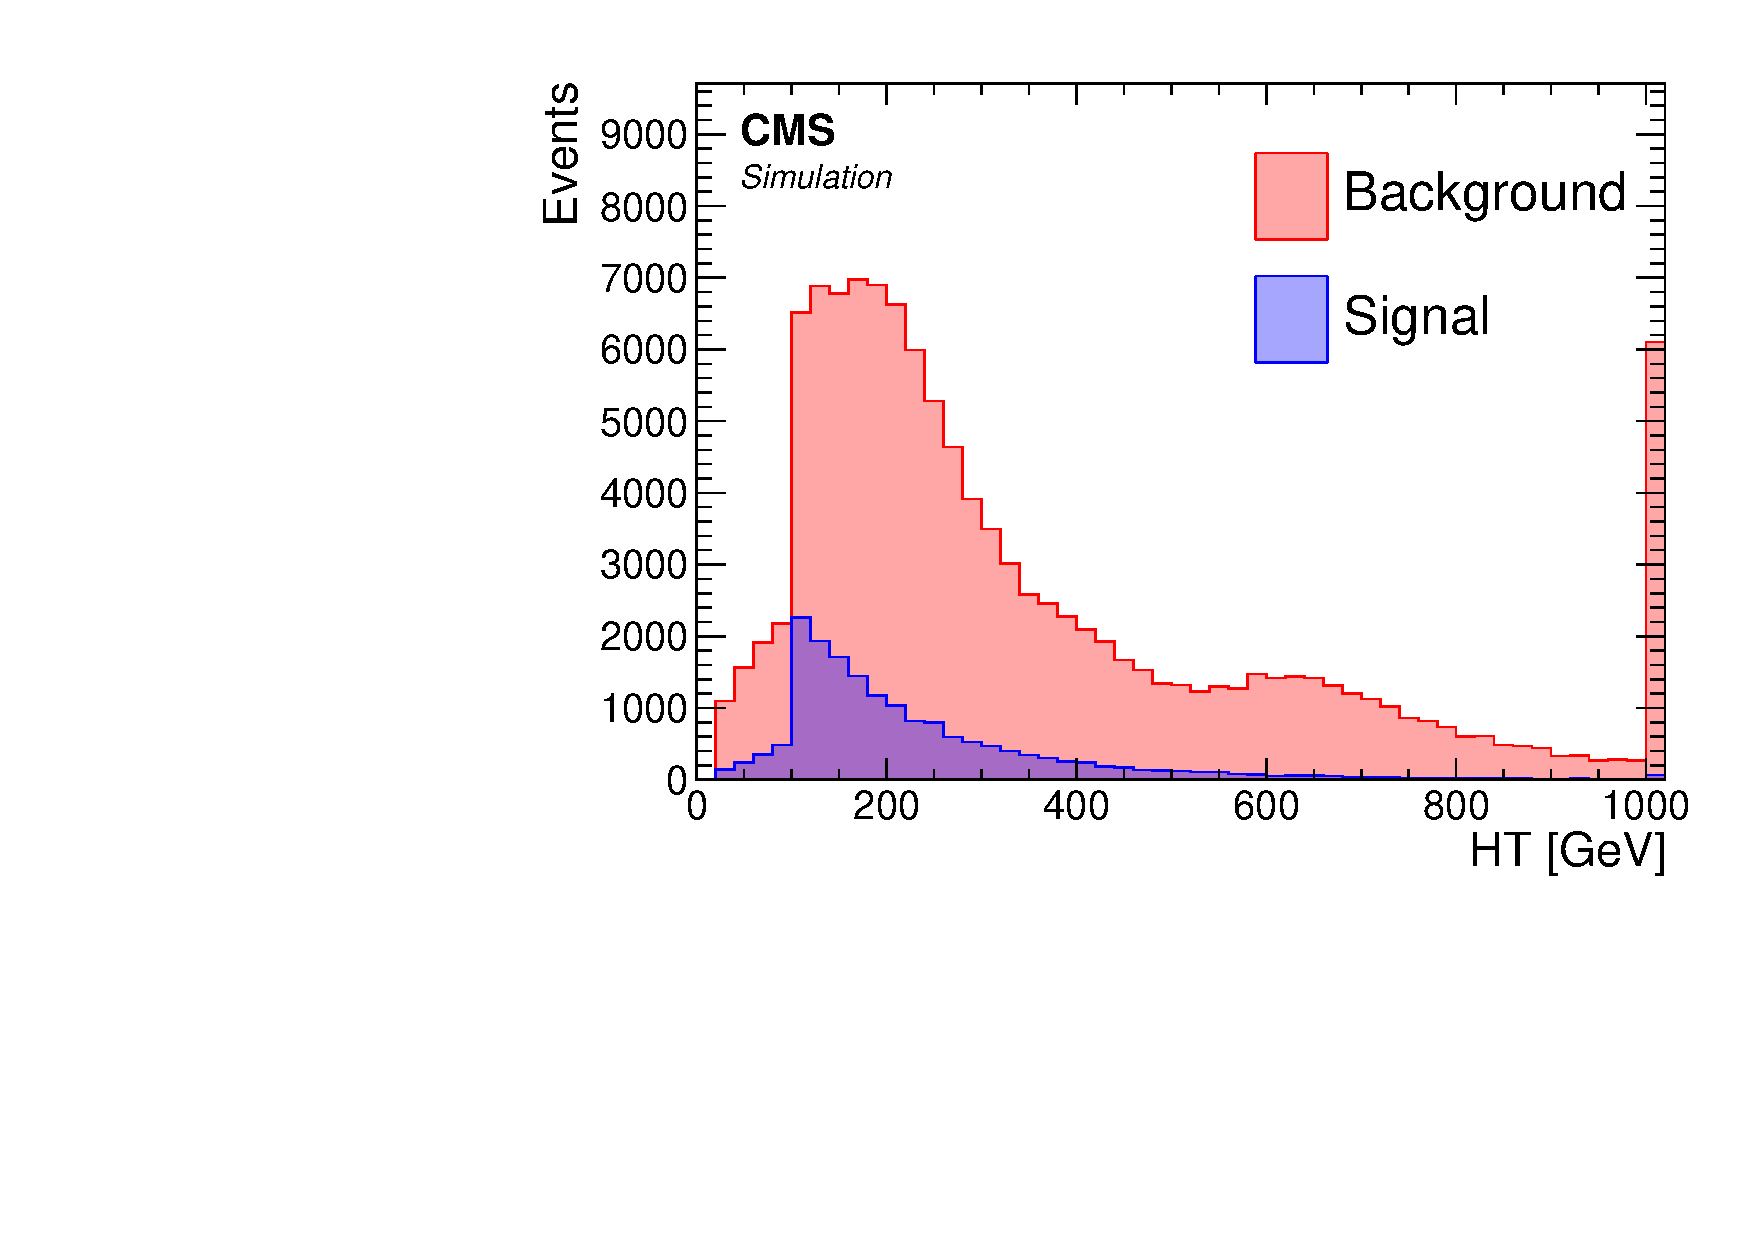
\includegraphics[width=0.32\linewidth]{plots/extrack_bdt_inputs_muons/none_HT.pdf} \,
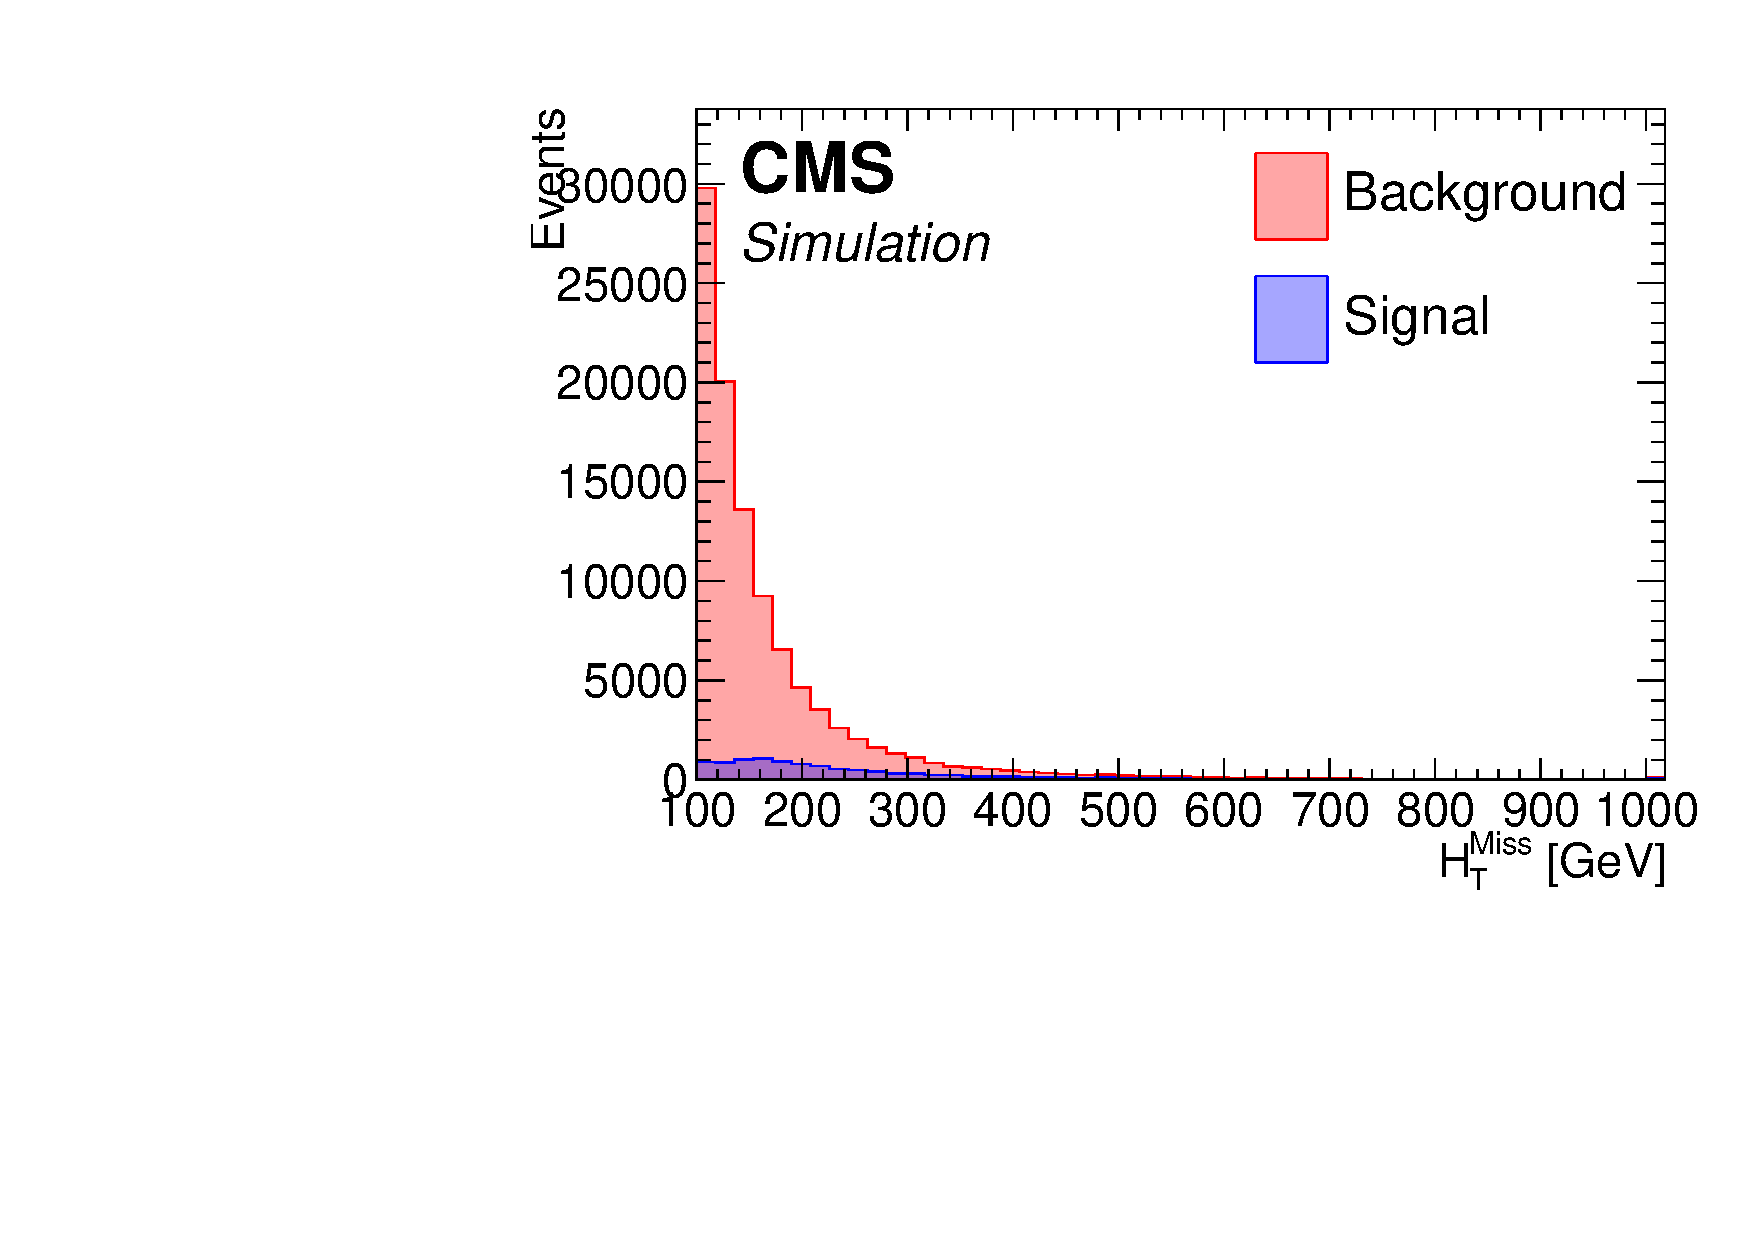
\includegraphics[width=0.32\linewidth]{plots/extrack_bdt_inputs_muons/none_MHT.pdf}  \,
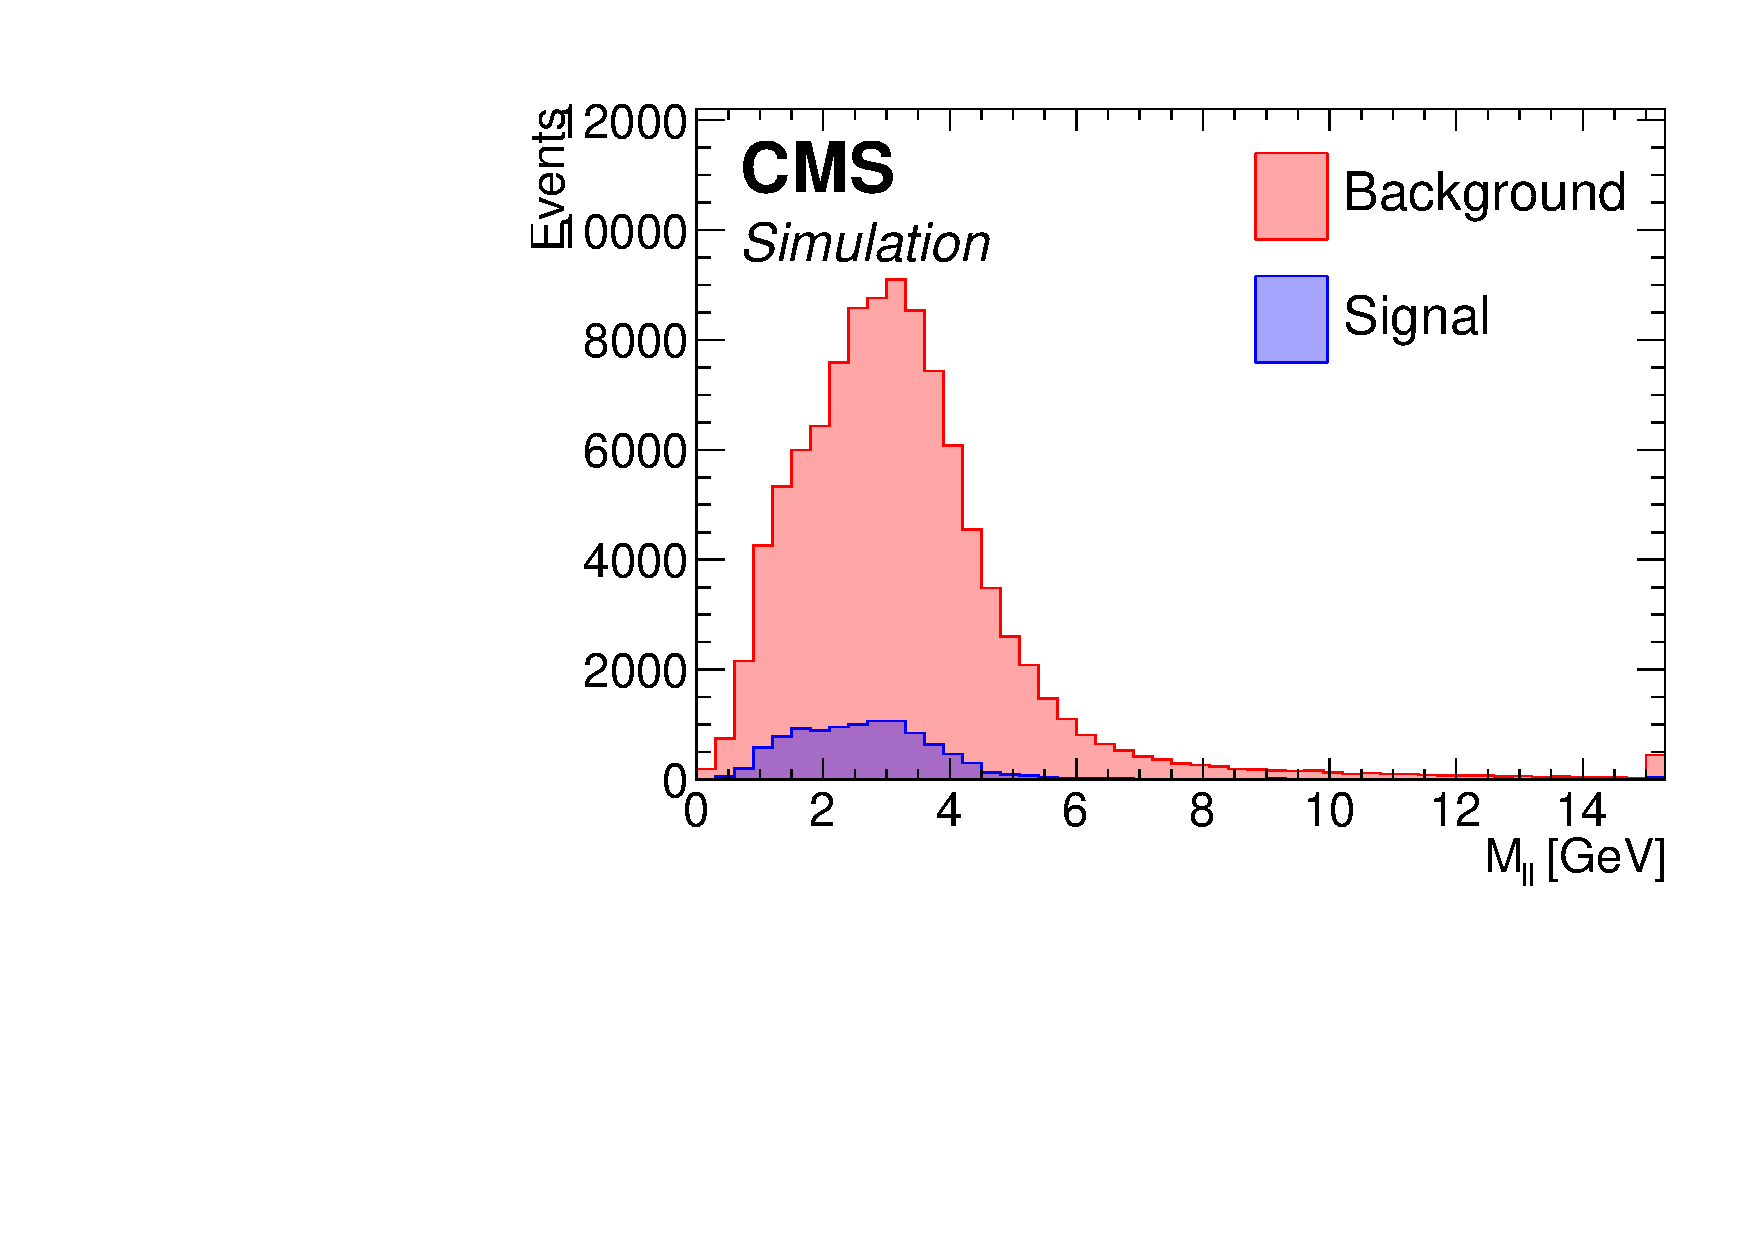
\includegraphics[width=0.32\linewidth]{plots/extrack_bdt_inputs_muons/none_exTrack_invMassCorrJetNoMultIso10Dr0.6.pdf} \\


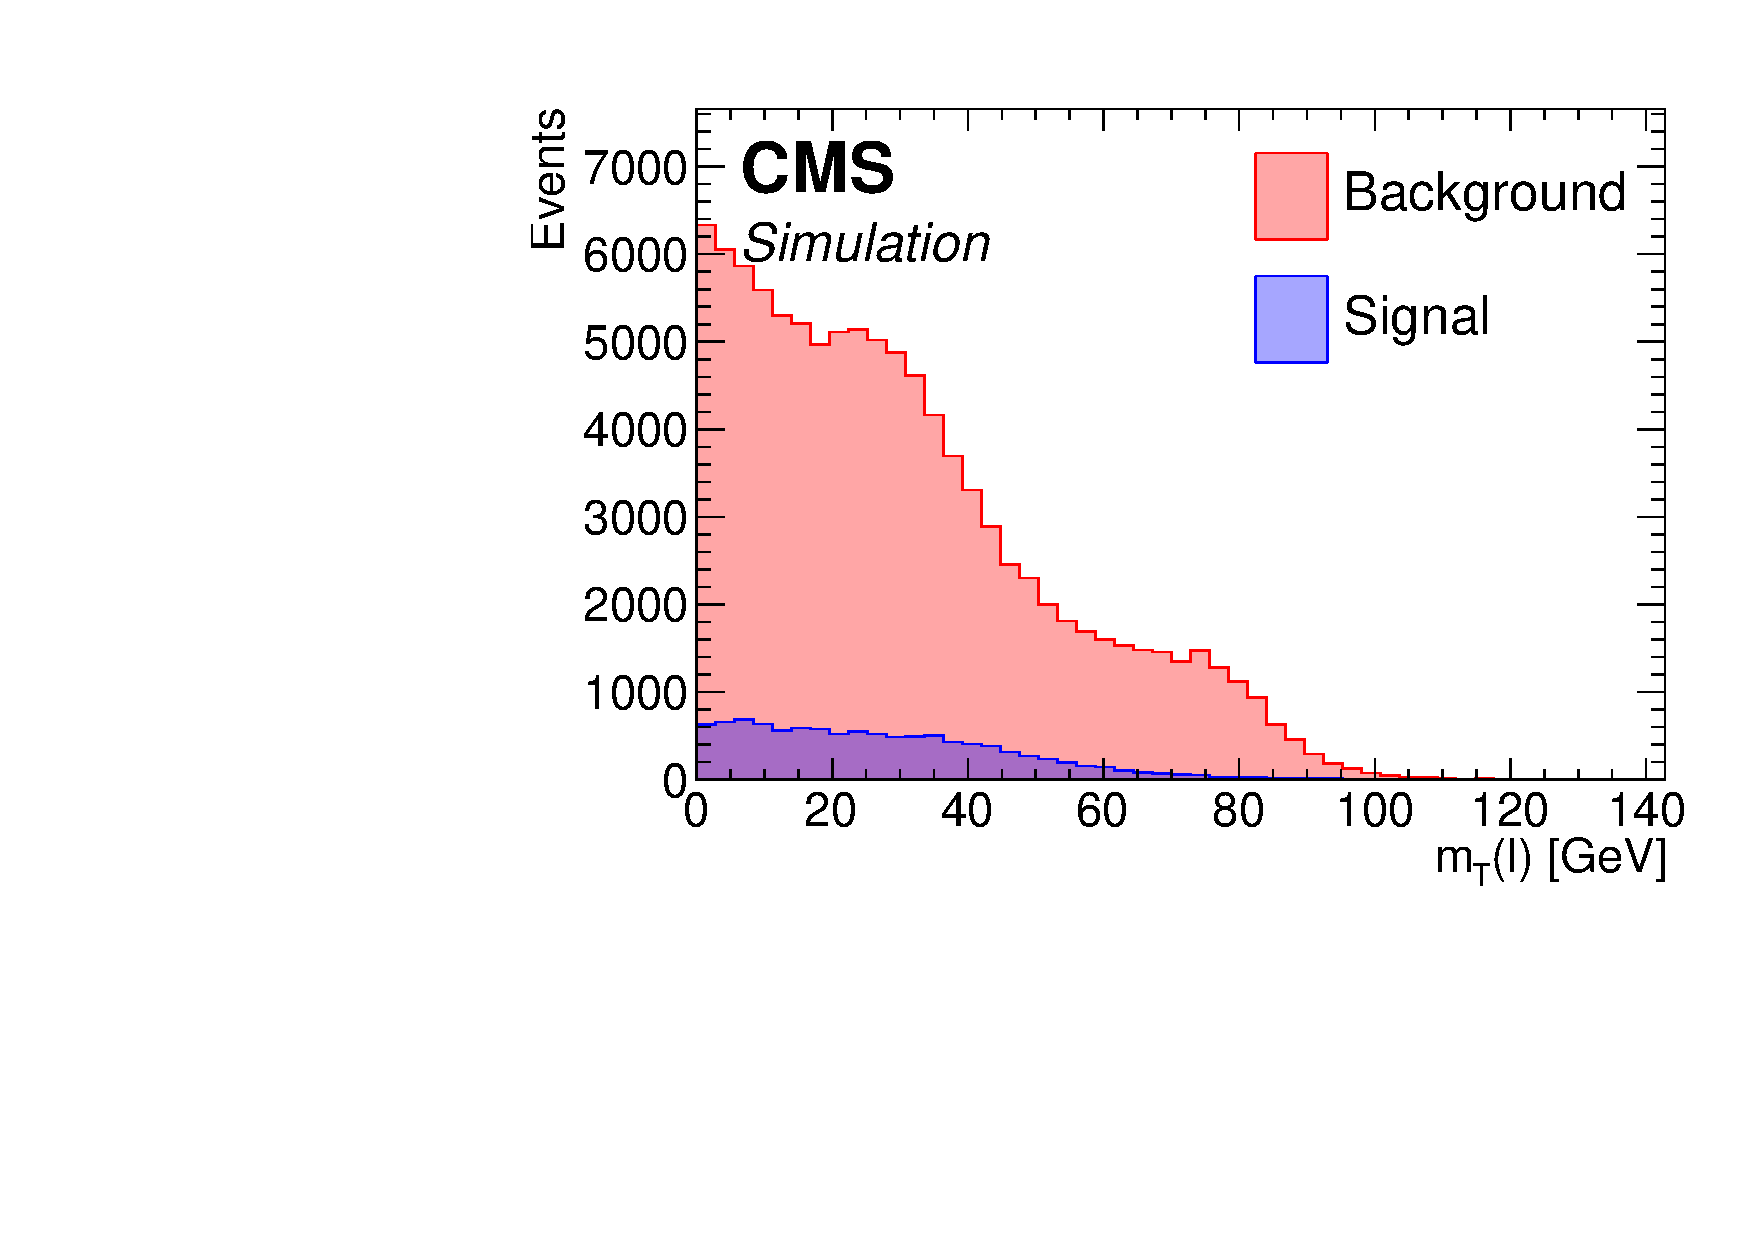
\includegraphics[width=0.32\linewidth]{plots/extrack_bdt_inputs_muons/none_mtlCorrJetNoMultIso10Dr0.6.pdf} \,
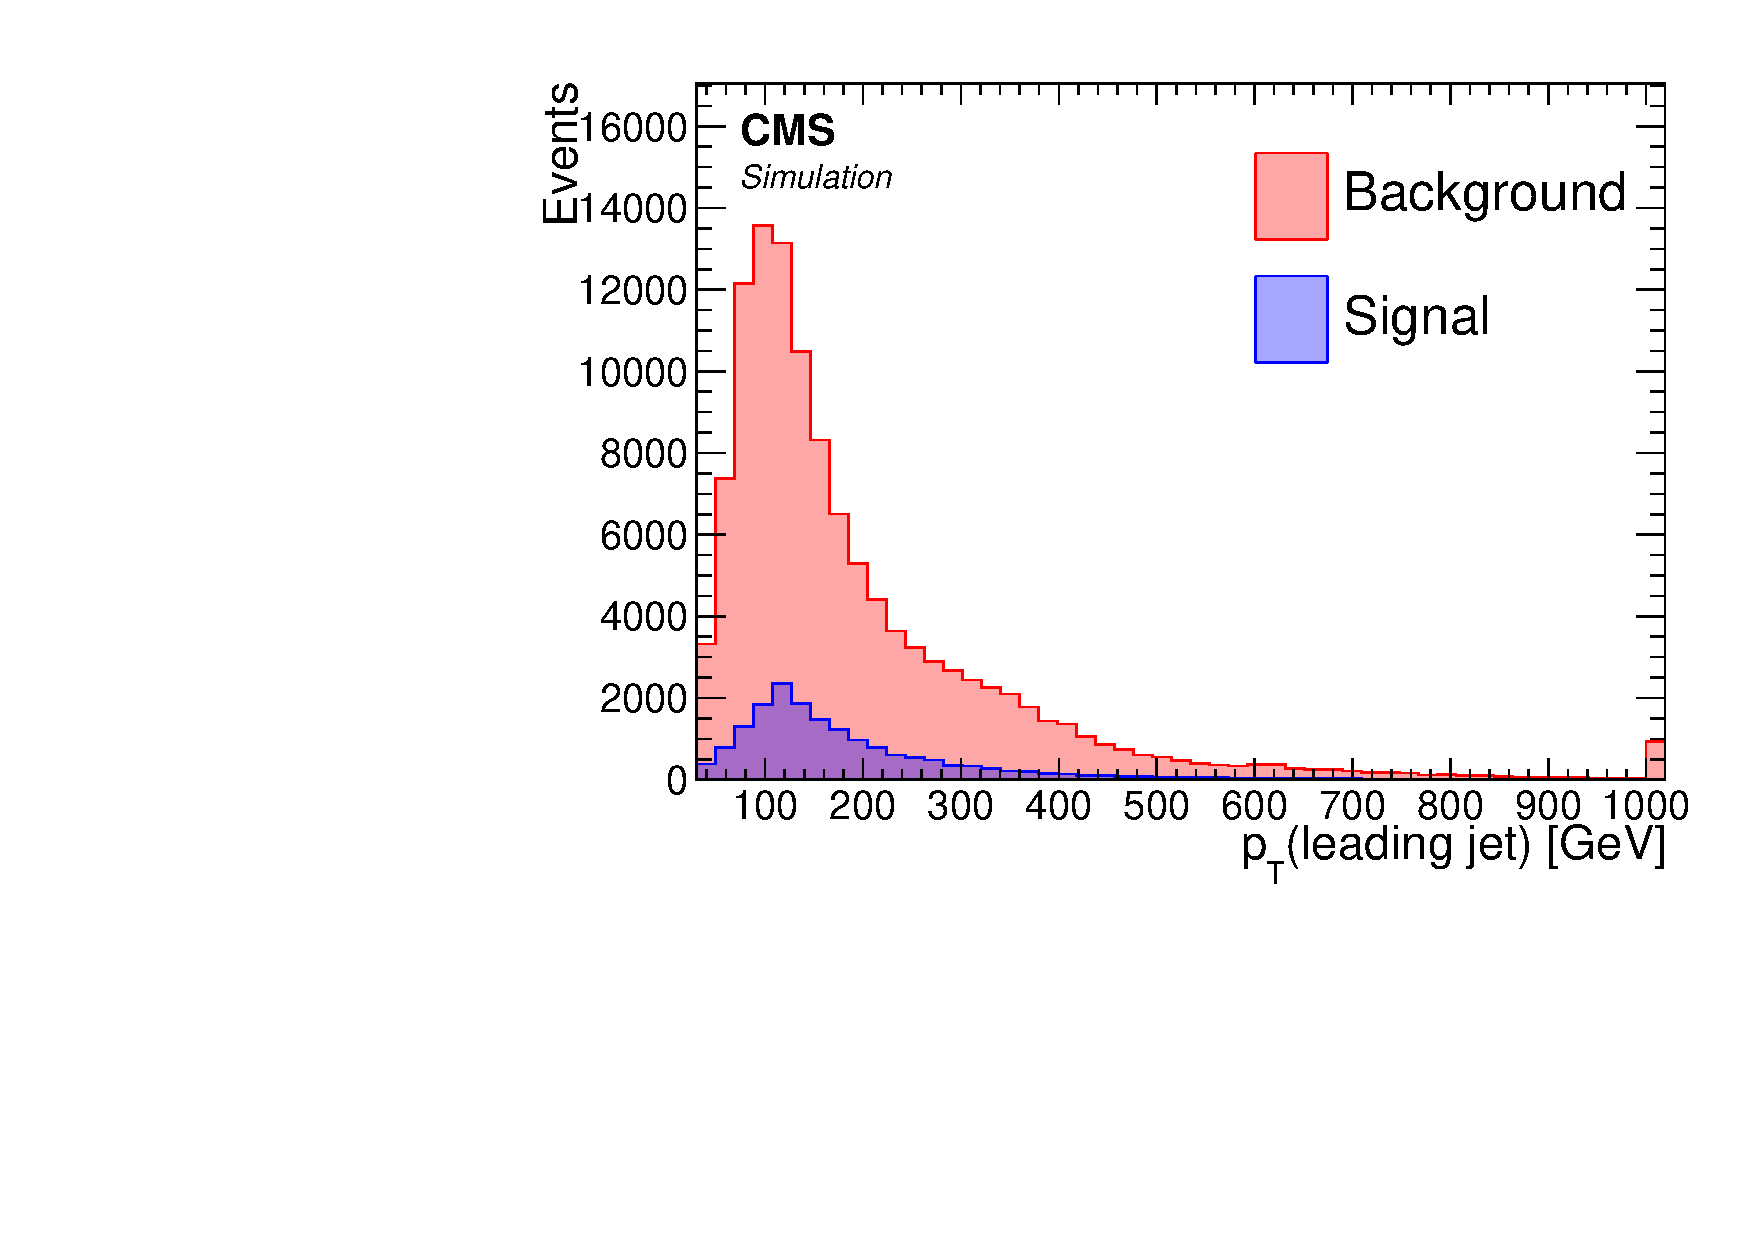
\includegraphics[width=0.32\linewidth]{plots/extrack_bdt_inputs_muons/none_LeadingJetPt.pdf} \,
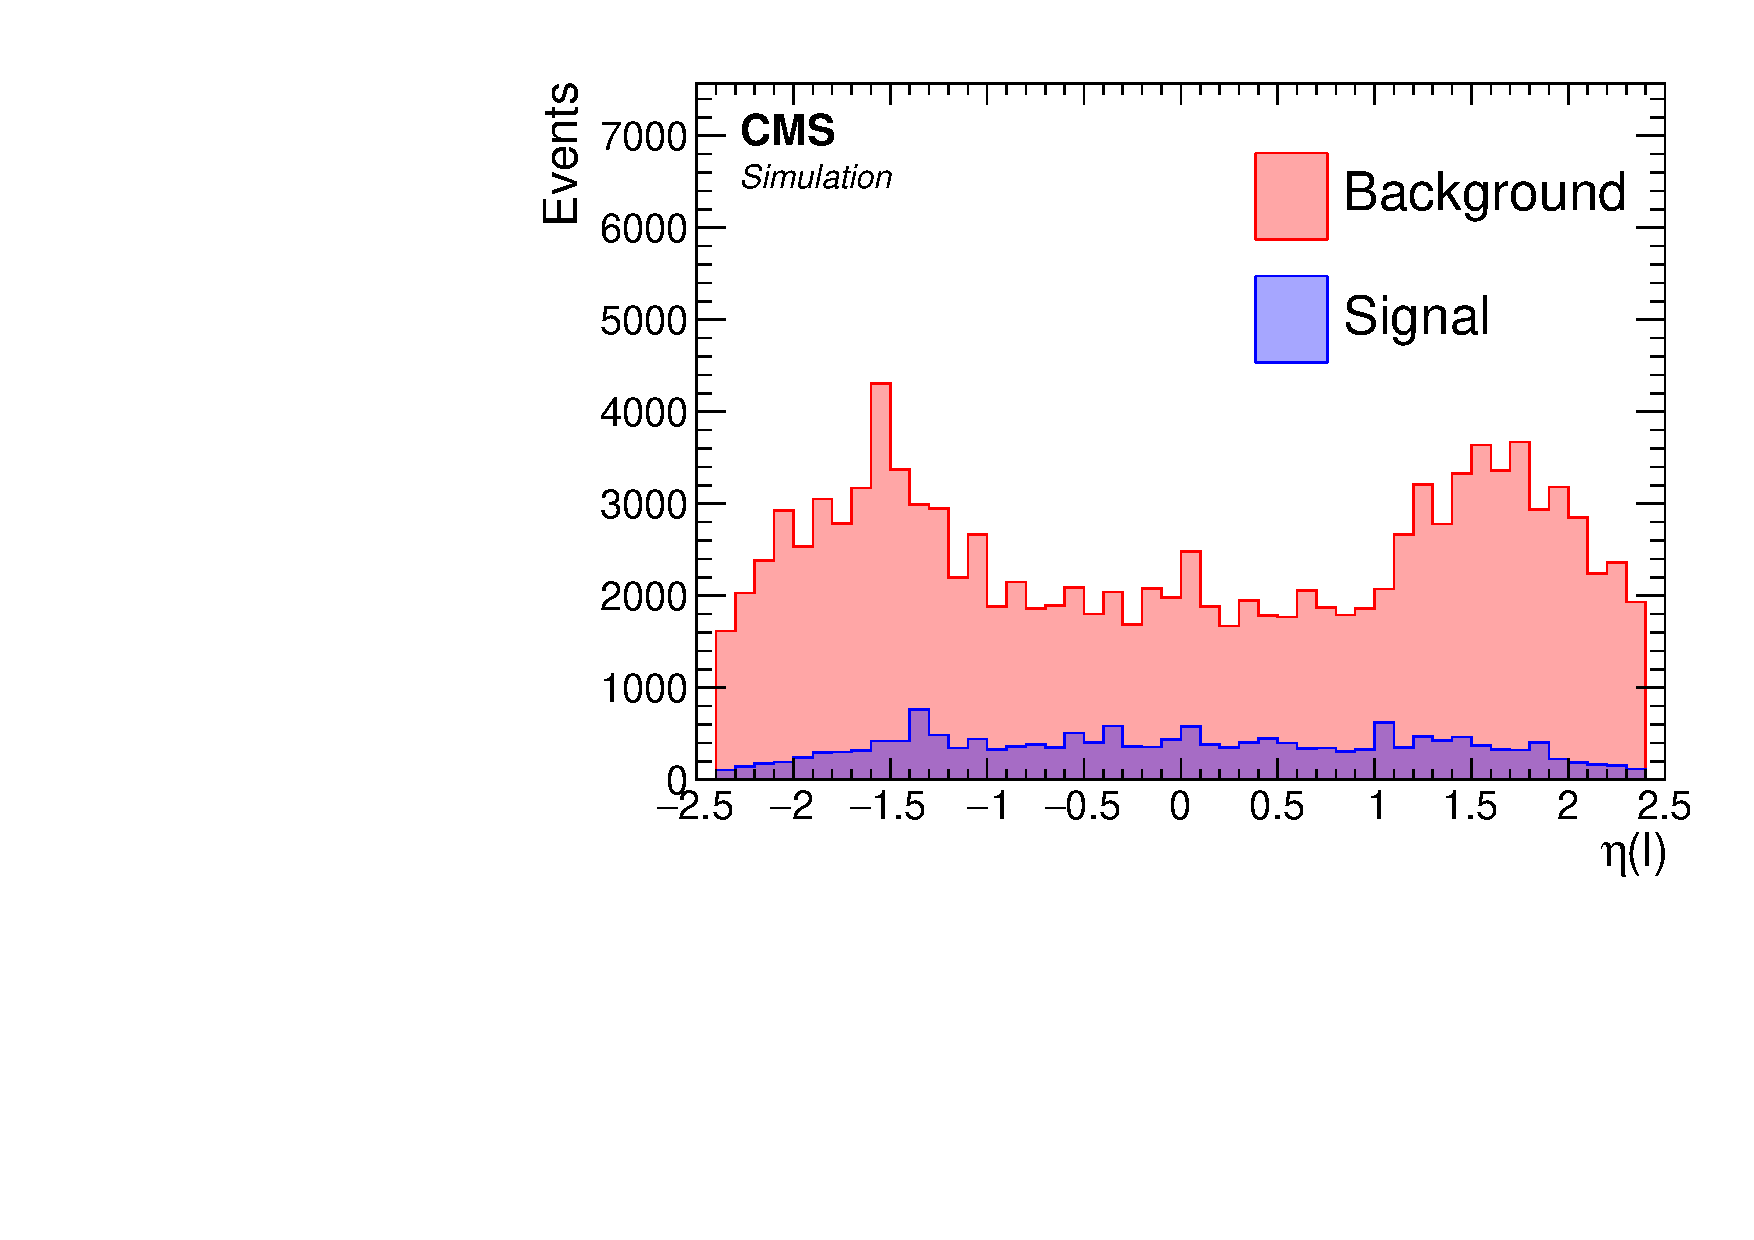
\includegraphics[width=0.32\linewidth]{plots/extrack_bdt_inputs_muons/none_leptonCorrJetNoMultIso10Dr0.6.Eta__.pdf}   \\
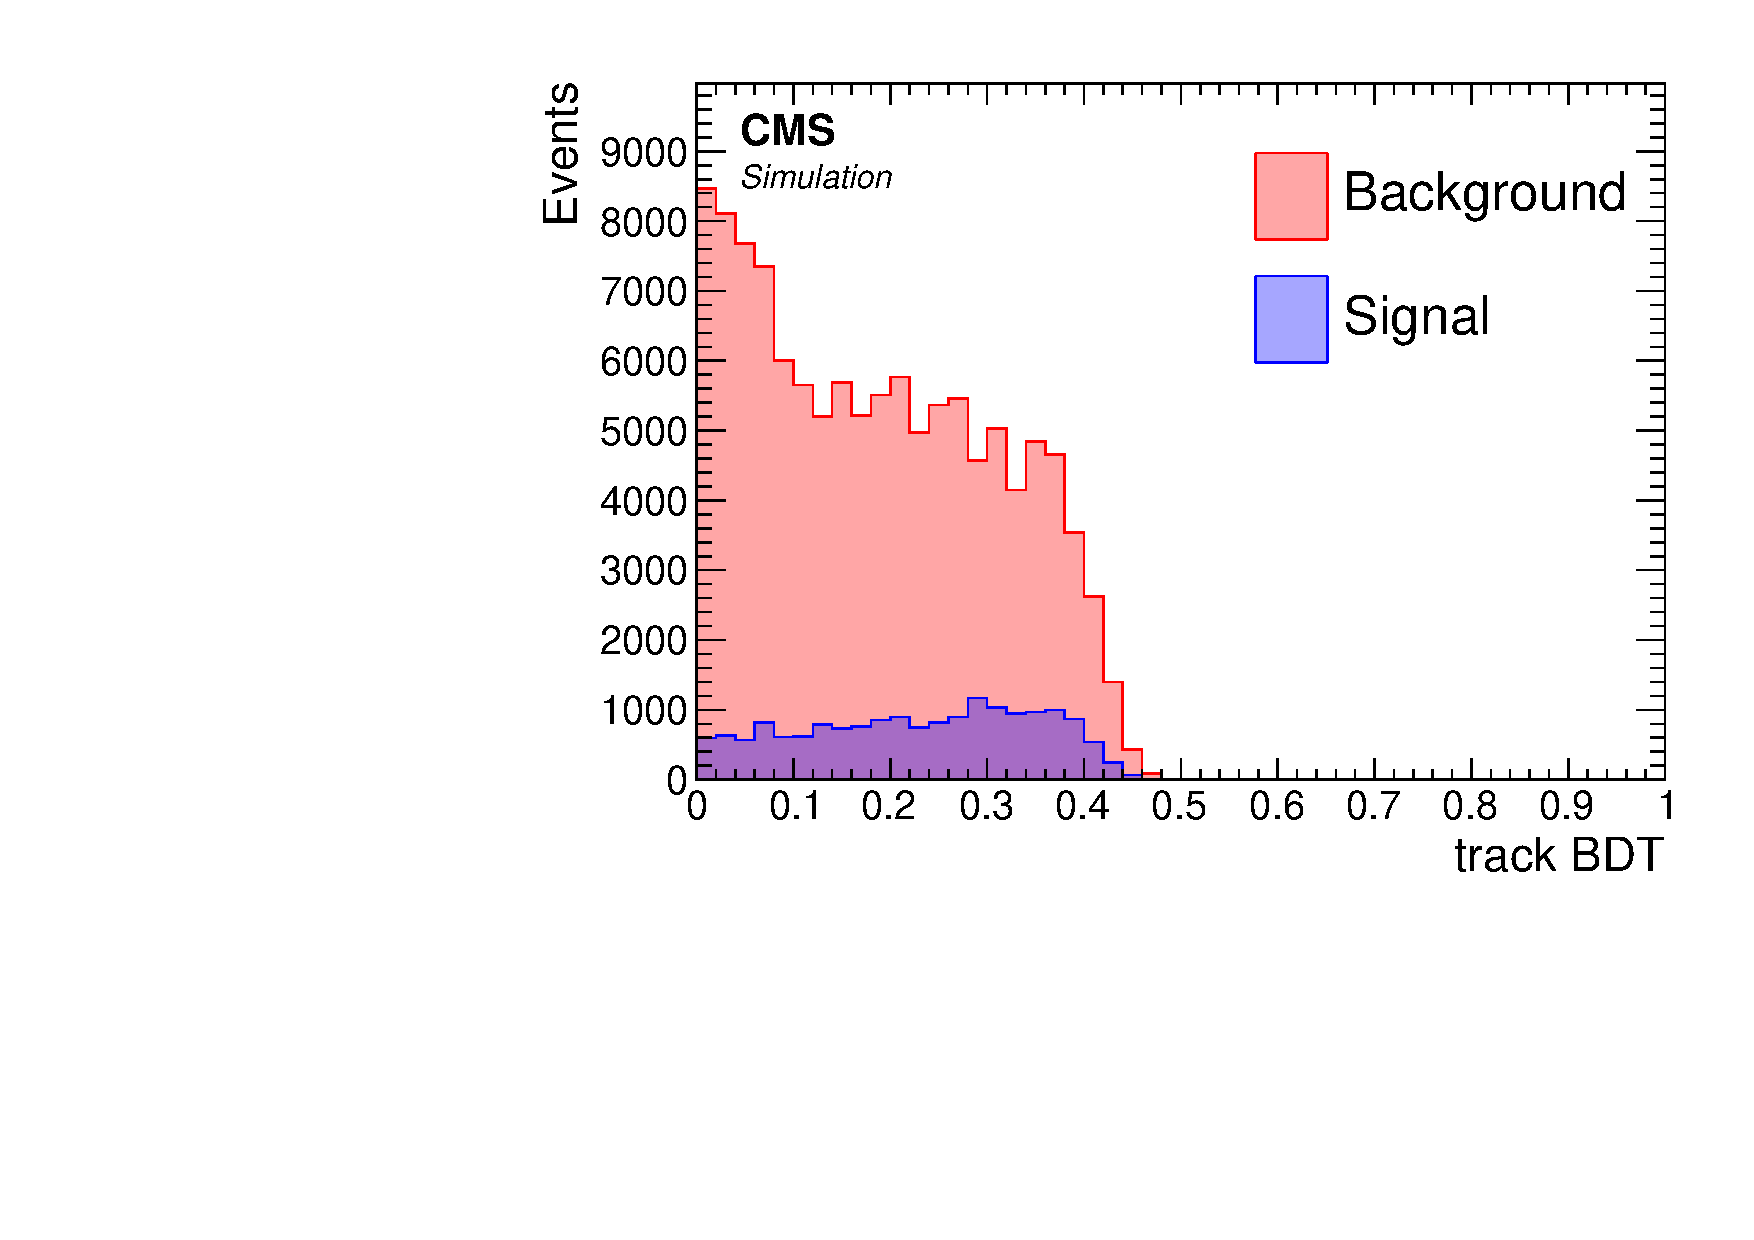
\includegraphics[width=0.32\linewidth]{plots/extrack_bdt_inputs_muons/none_trackBDTCorrJetNoMultIso10Dr0.6.pdf} \,
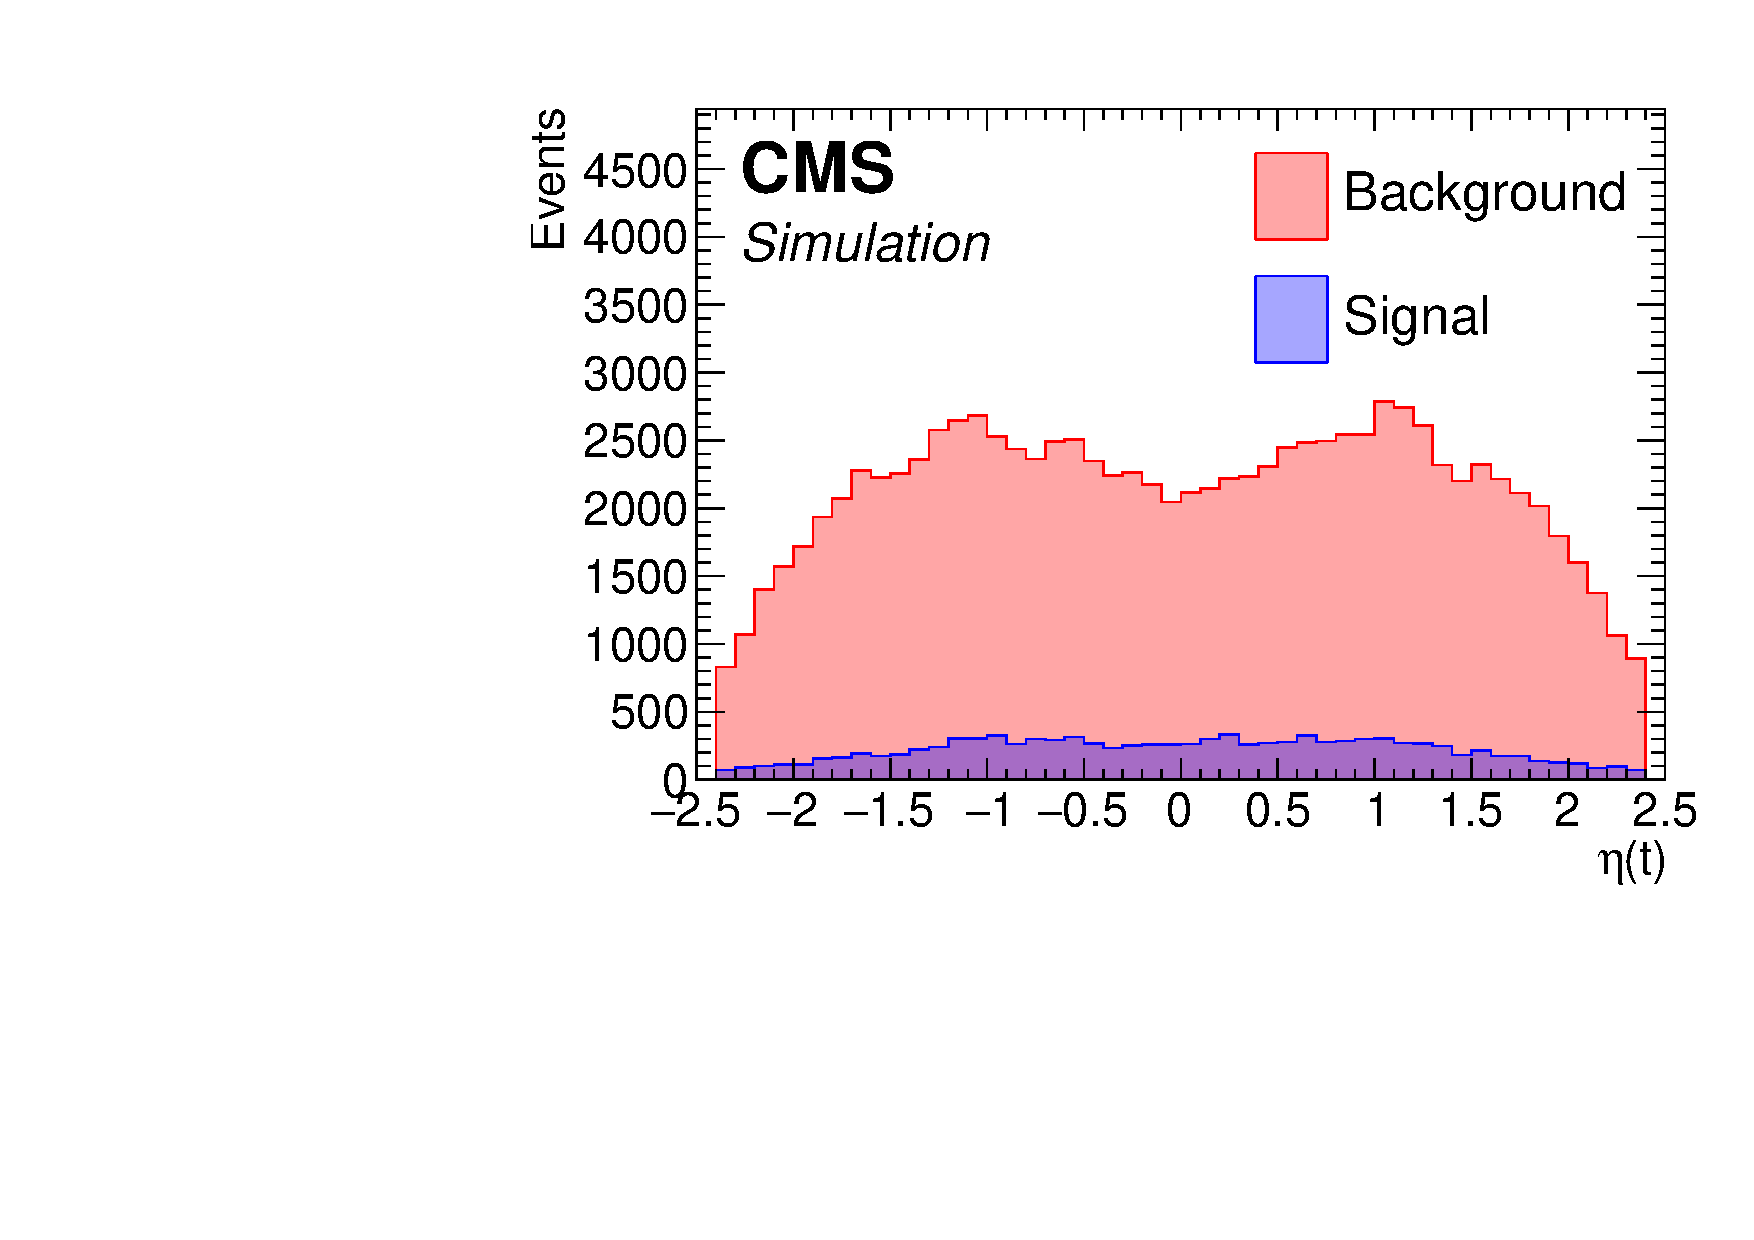
\includegraphics[width=0.32\linewidth]{plots/extrack_bdt_inputs_muons/none_trackCorrJetNoMultIso10Dr0.6.Eta__.pdf}  \,
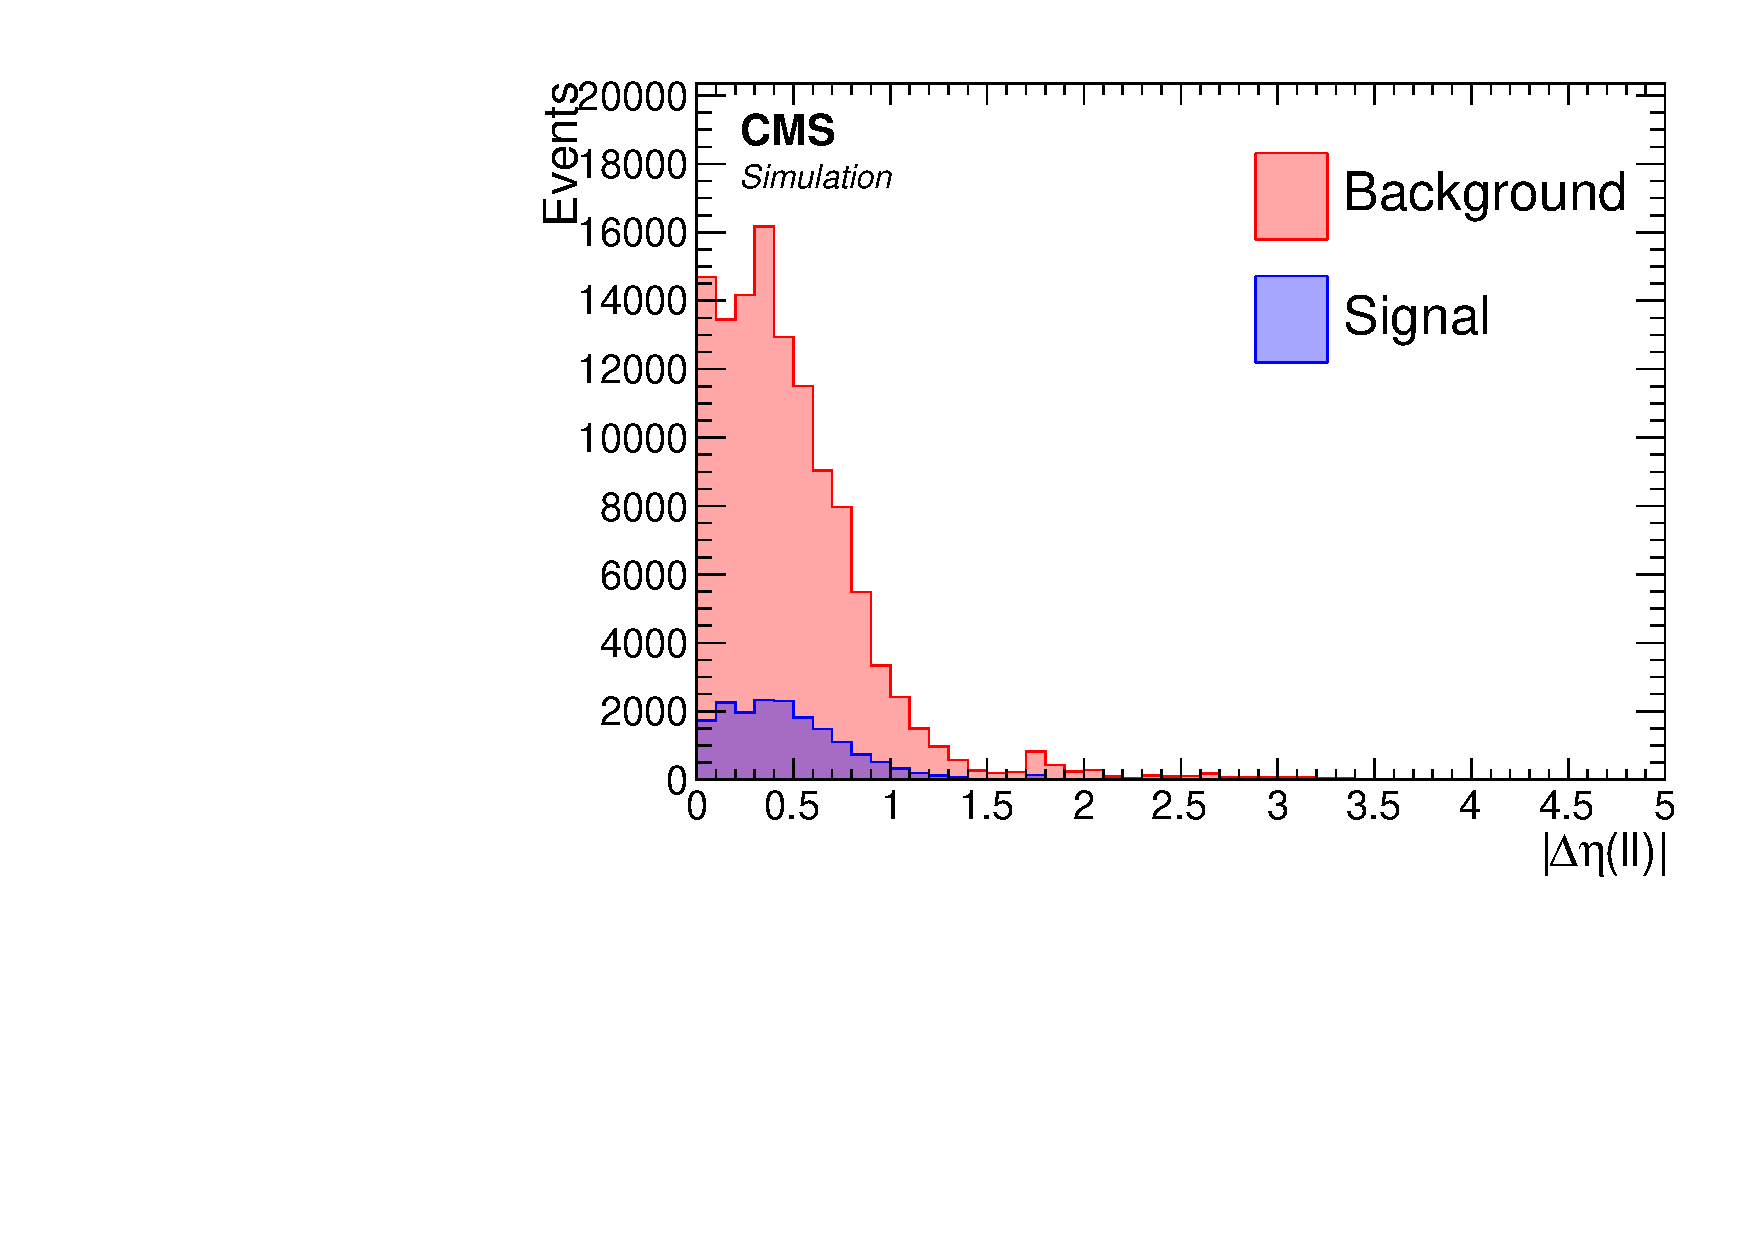
\includegraphics[width=0.32\linewidth]{plots/extrack_bdt_inputs_muons/none_exTrack_deltaEtaCorrJetNoMultIso10Dr0.6.pdf} \\


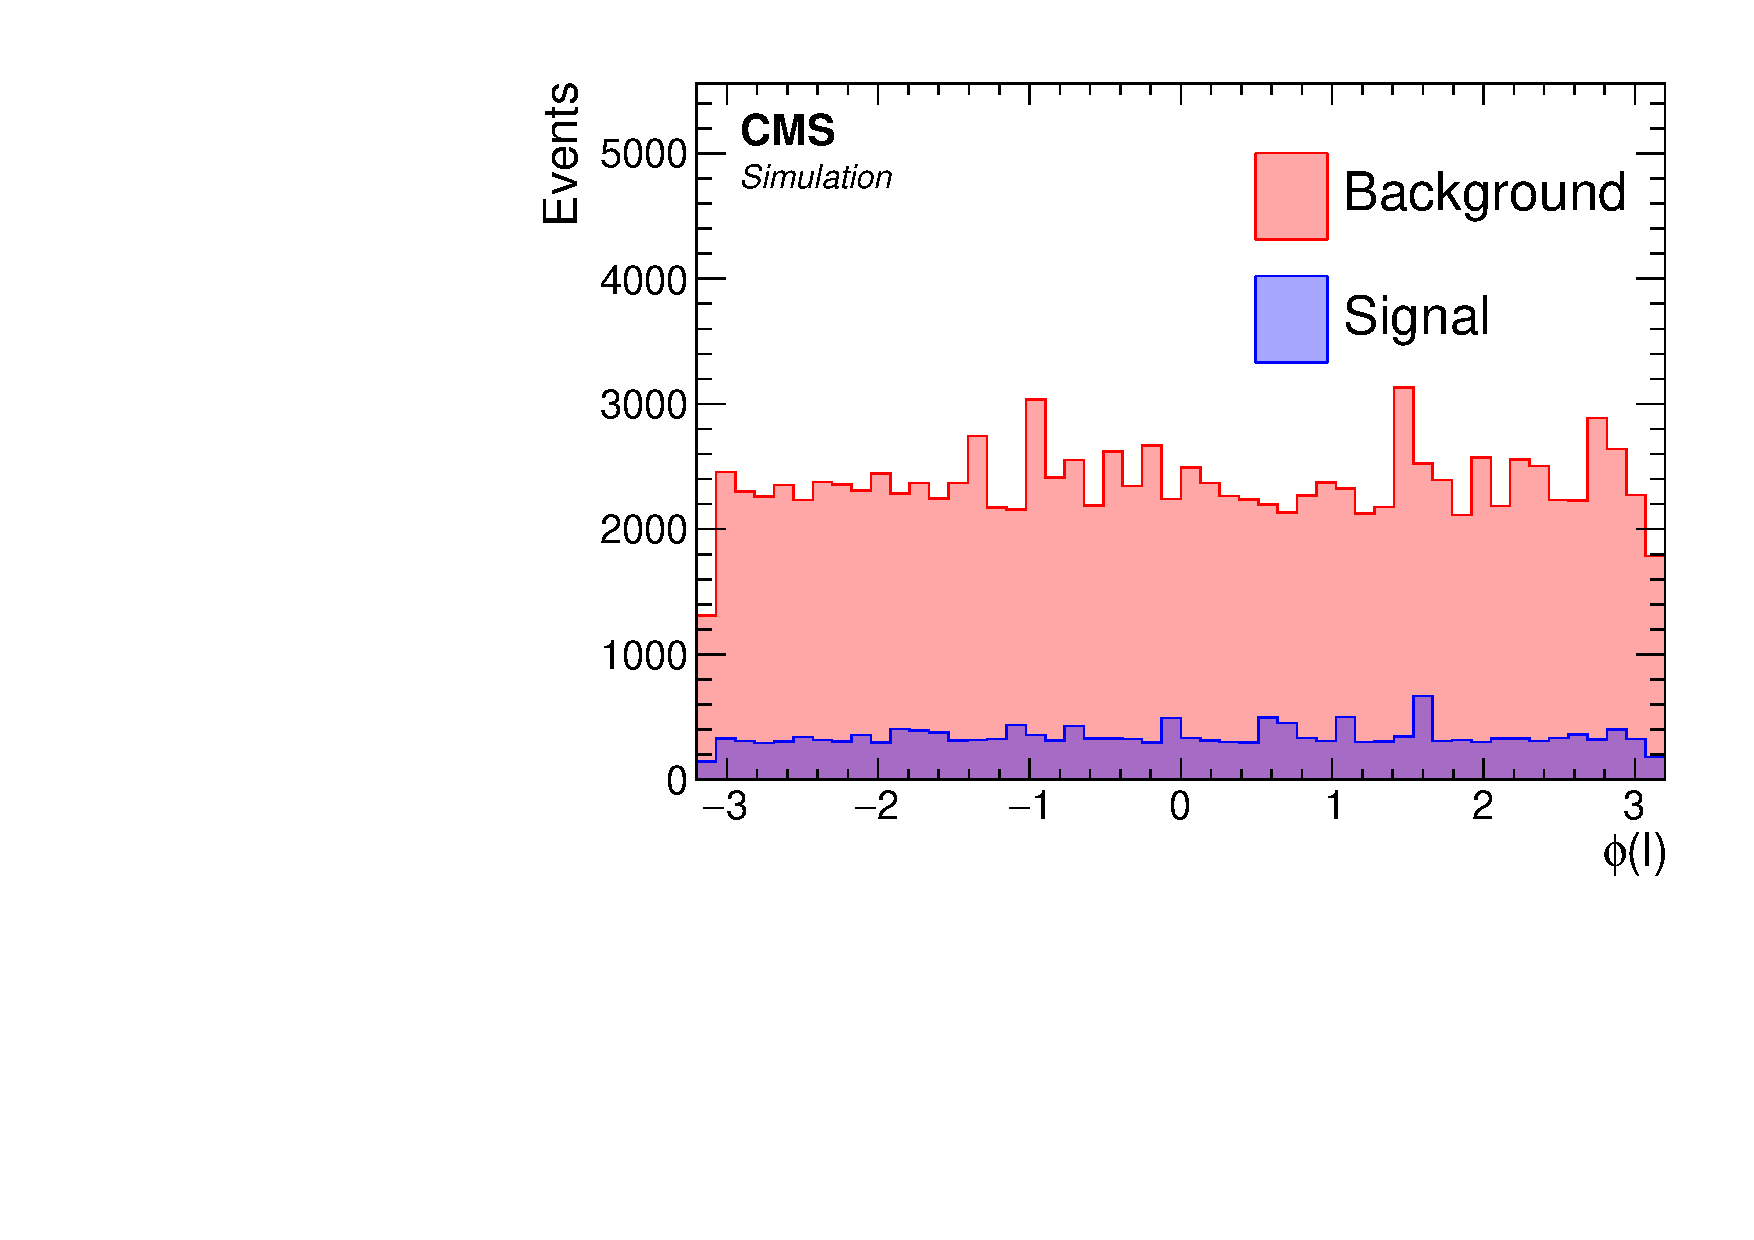
\includegraphics[width=0.32\linewidth]{plots/extrack_bdt_inputs_muons/none_leptonCorrJetNoMultIso10Dr0.6.Phi__.pdf} \,
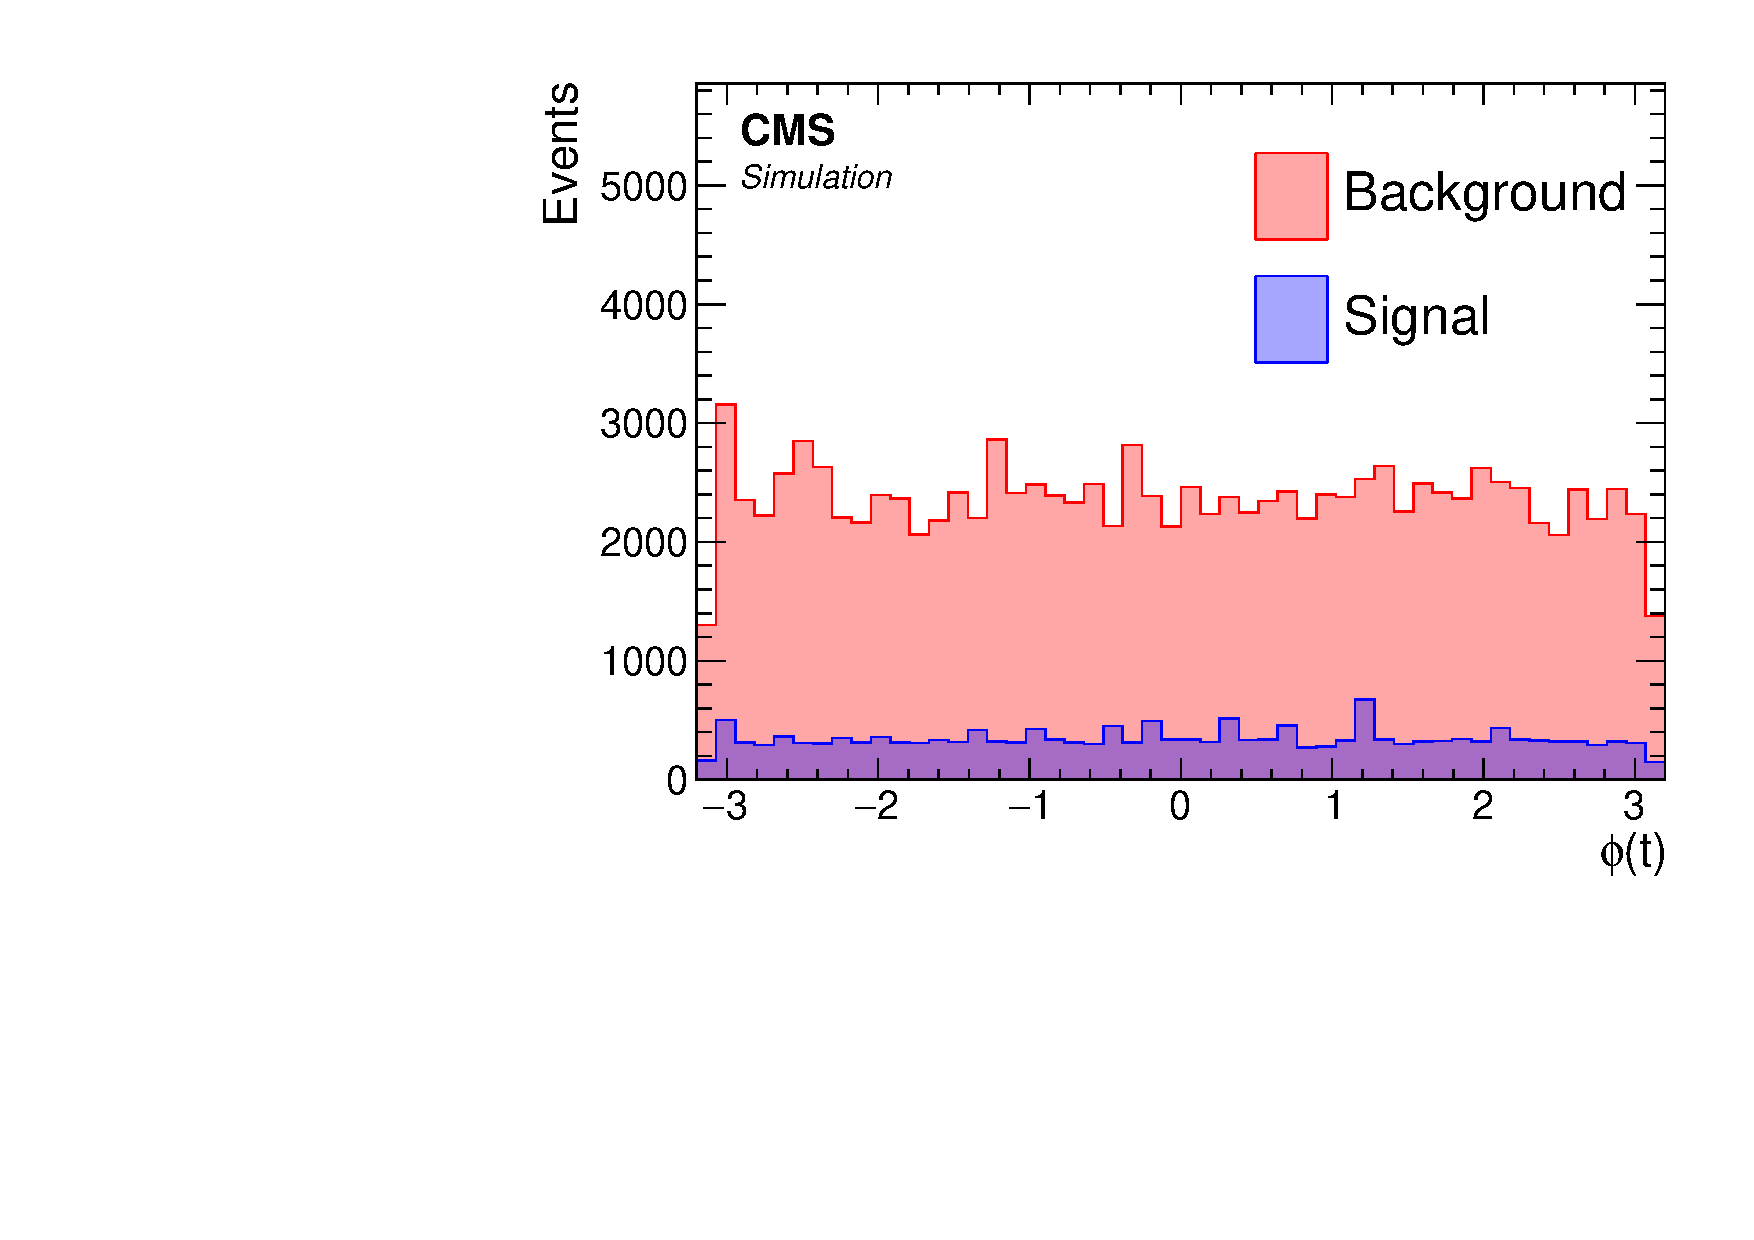
\includegraphics[width=0.32\linewidth]{plots/extrack_bdt_inputs_muons/none_trackCorrJetNoMultIso10Dr0.6.Phi__.pdf} \,
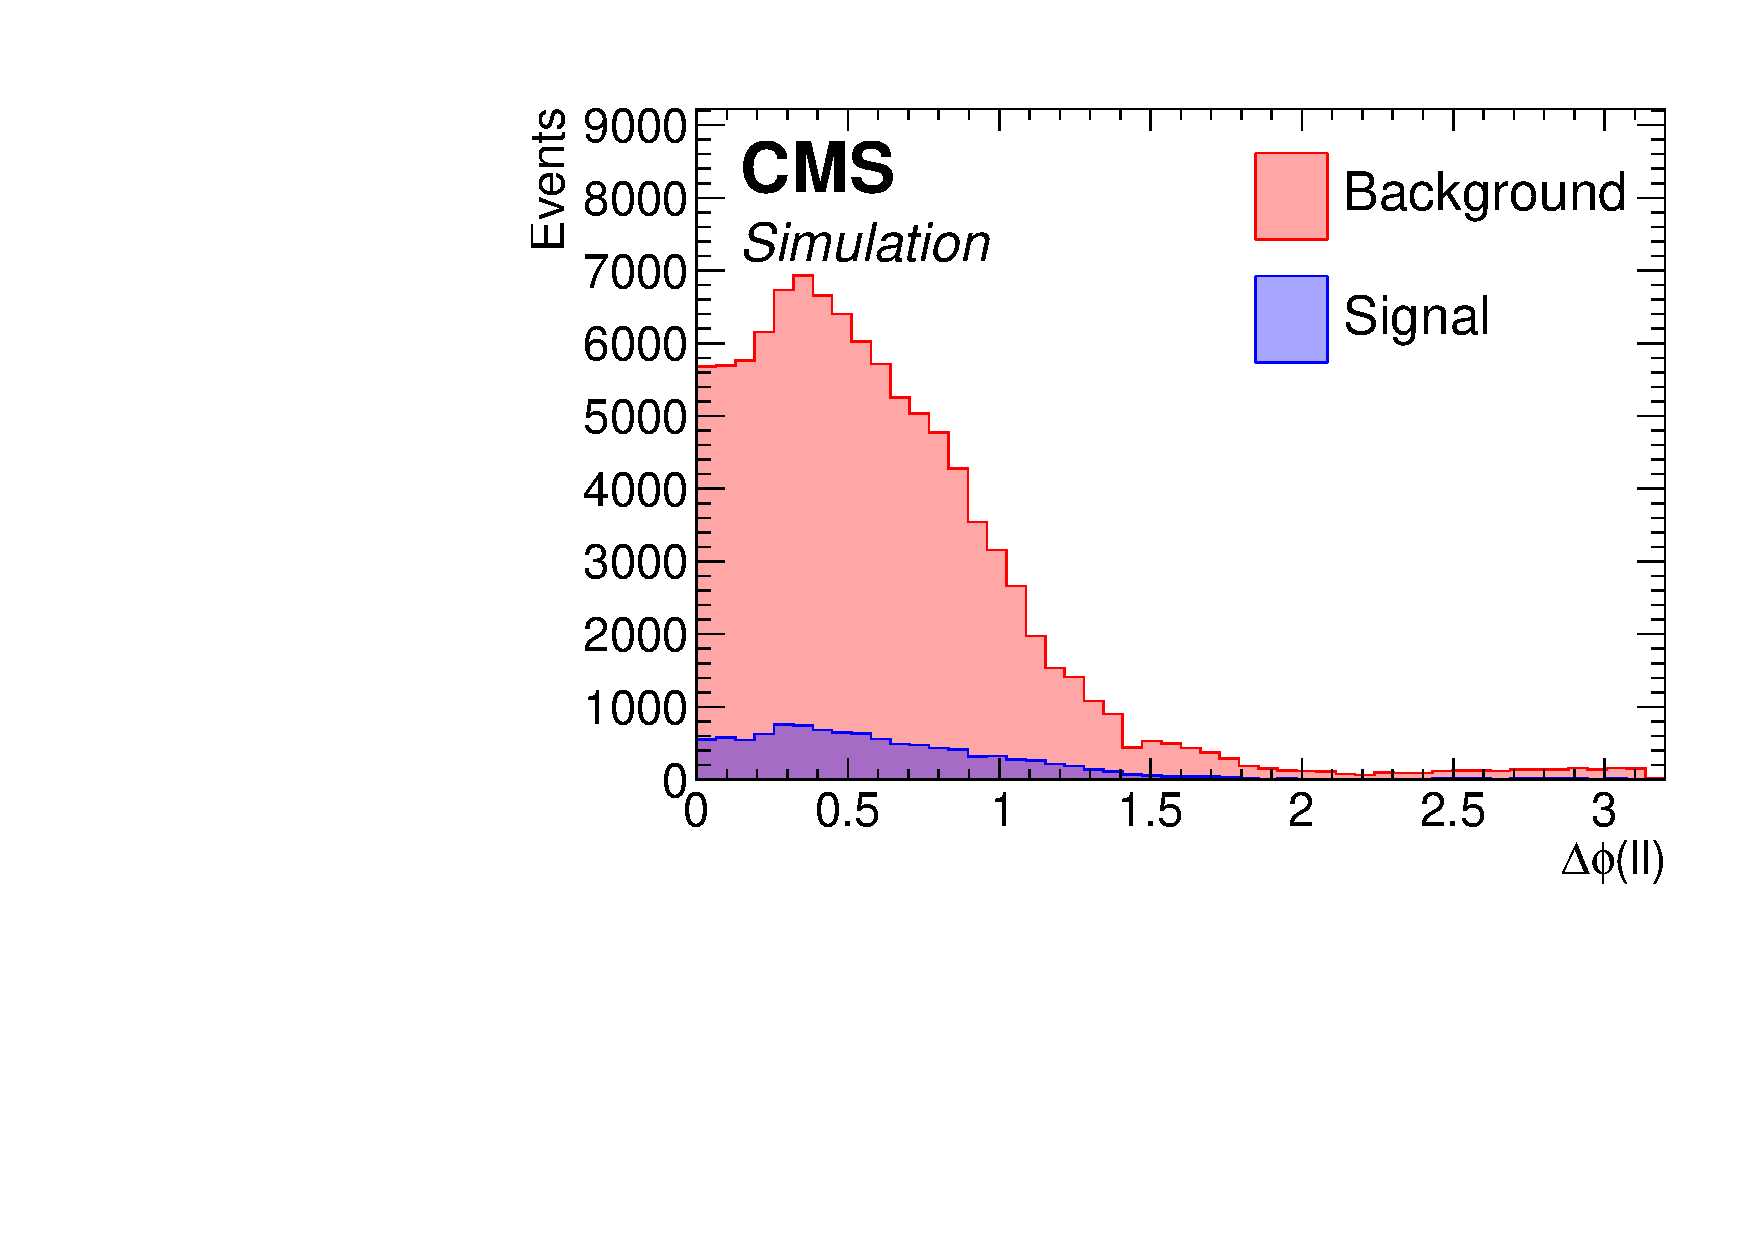
\includegraphics[width=0.32\linewidth]{plots/extrack_bdt_inputs_muons/none_exTrack_deltaPhiCorrJetNoMultIso10Dr0.6.pdf} \\
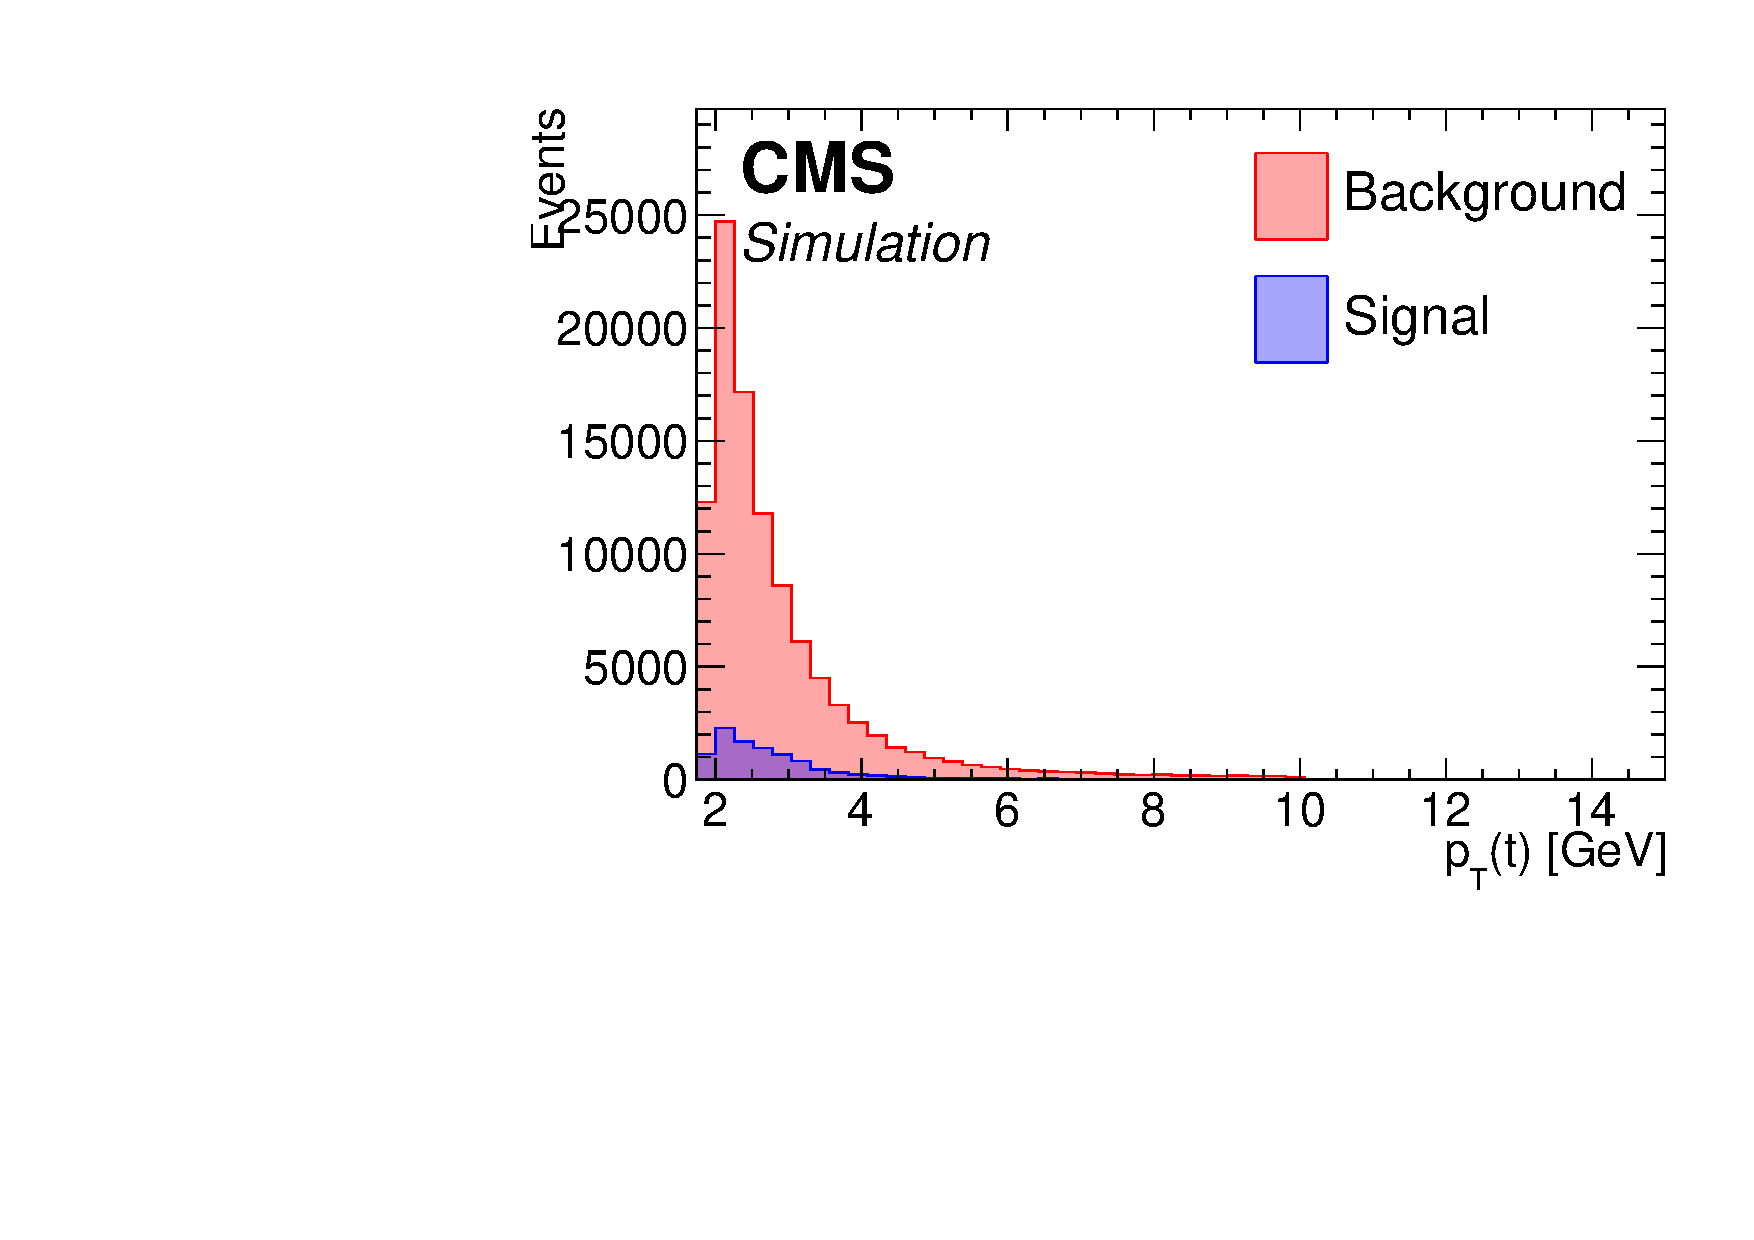
\includegraphics[width=0.32\linewidth]{plots/extrack_bdt_inputs_muons/none_trackCorrJetNoMultIso10Dr0.6.Pt__ .pdf}  \,
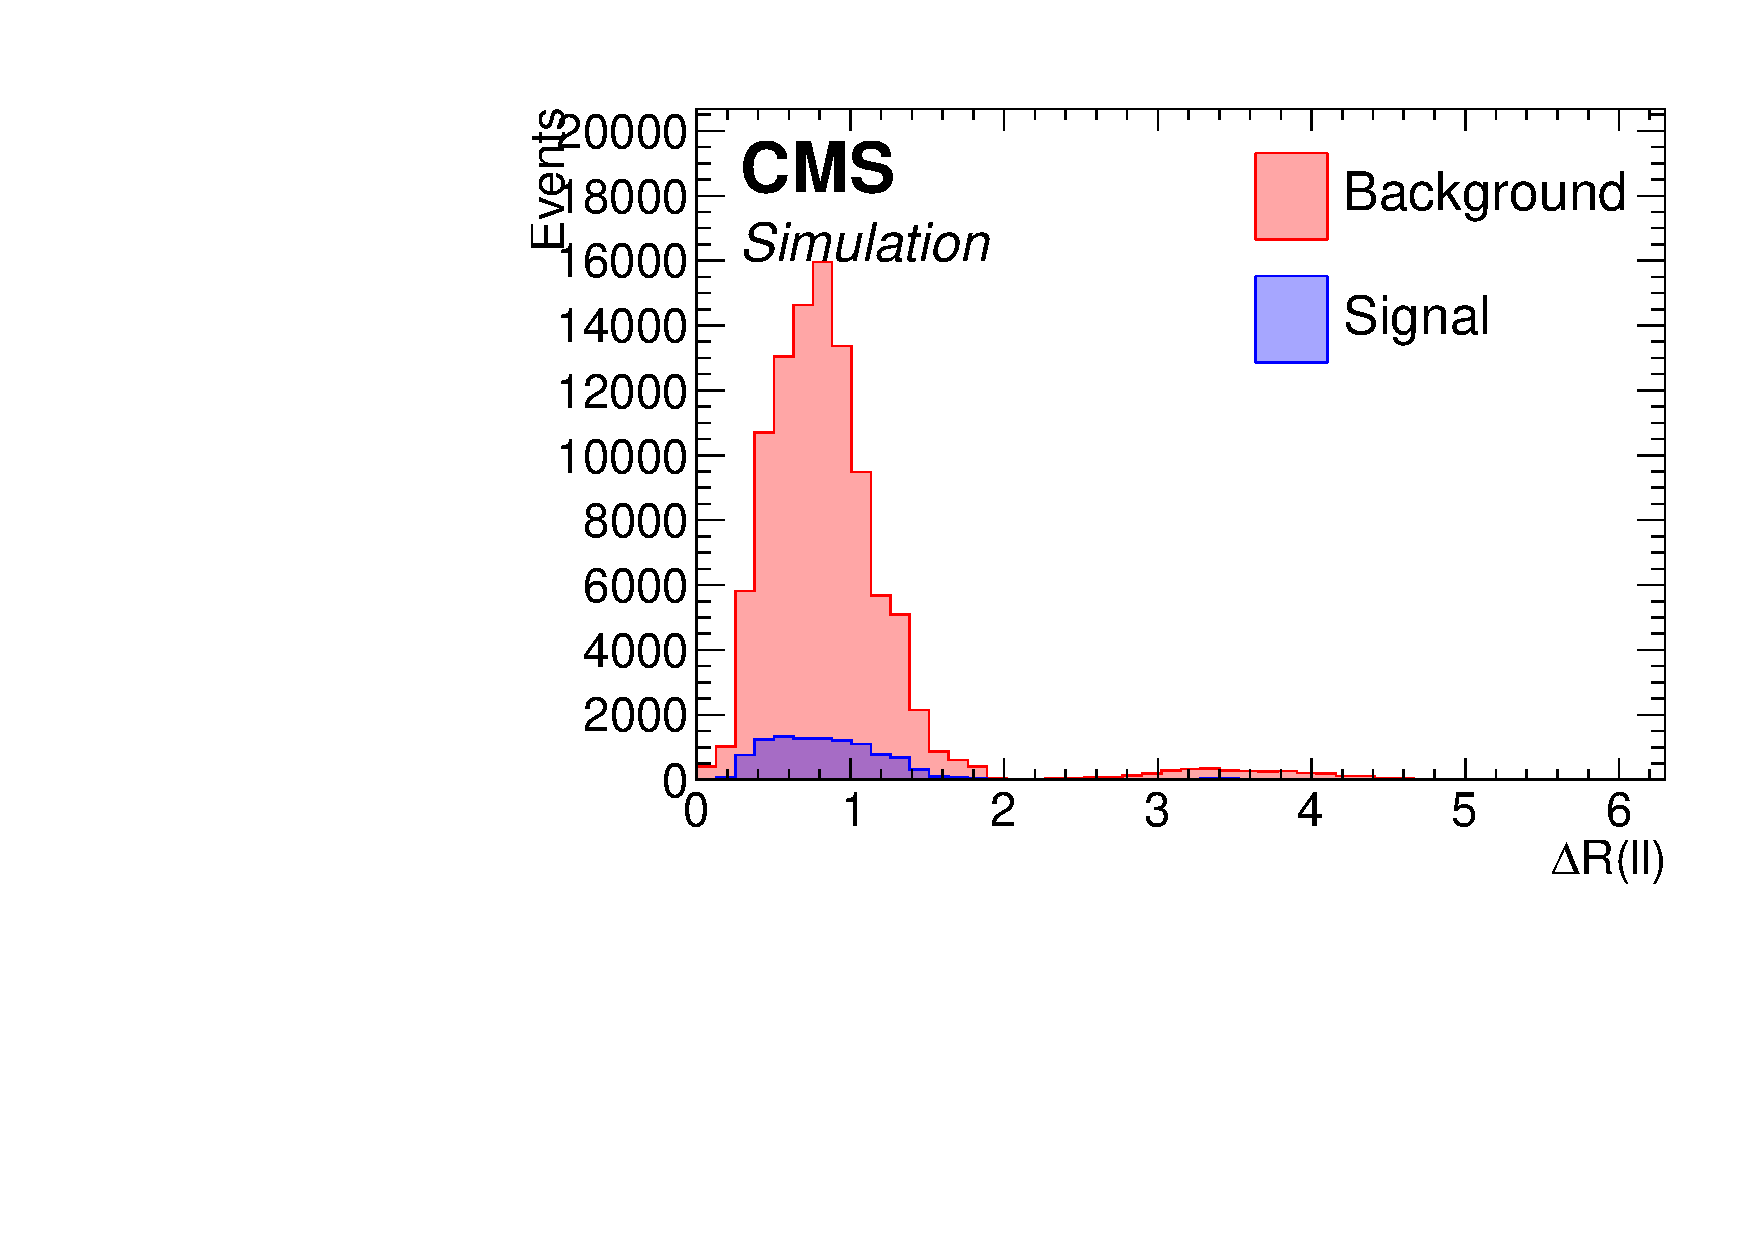
\includegraphics[width=0.32\linewidth]{plots/extrack_bdt_inputs_muons/none_exTrack_deltaRCorrJetNoMultIso10Dr0.6.pdf} \,
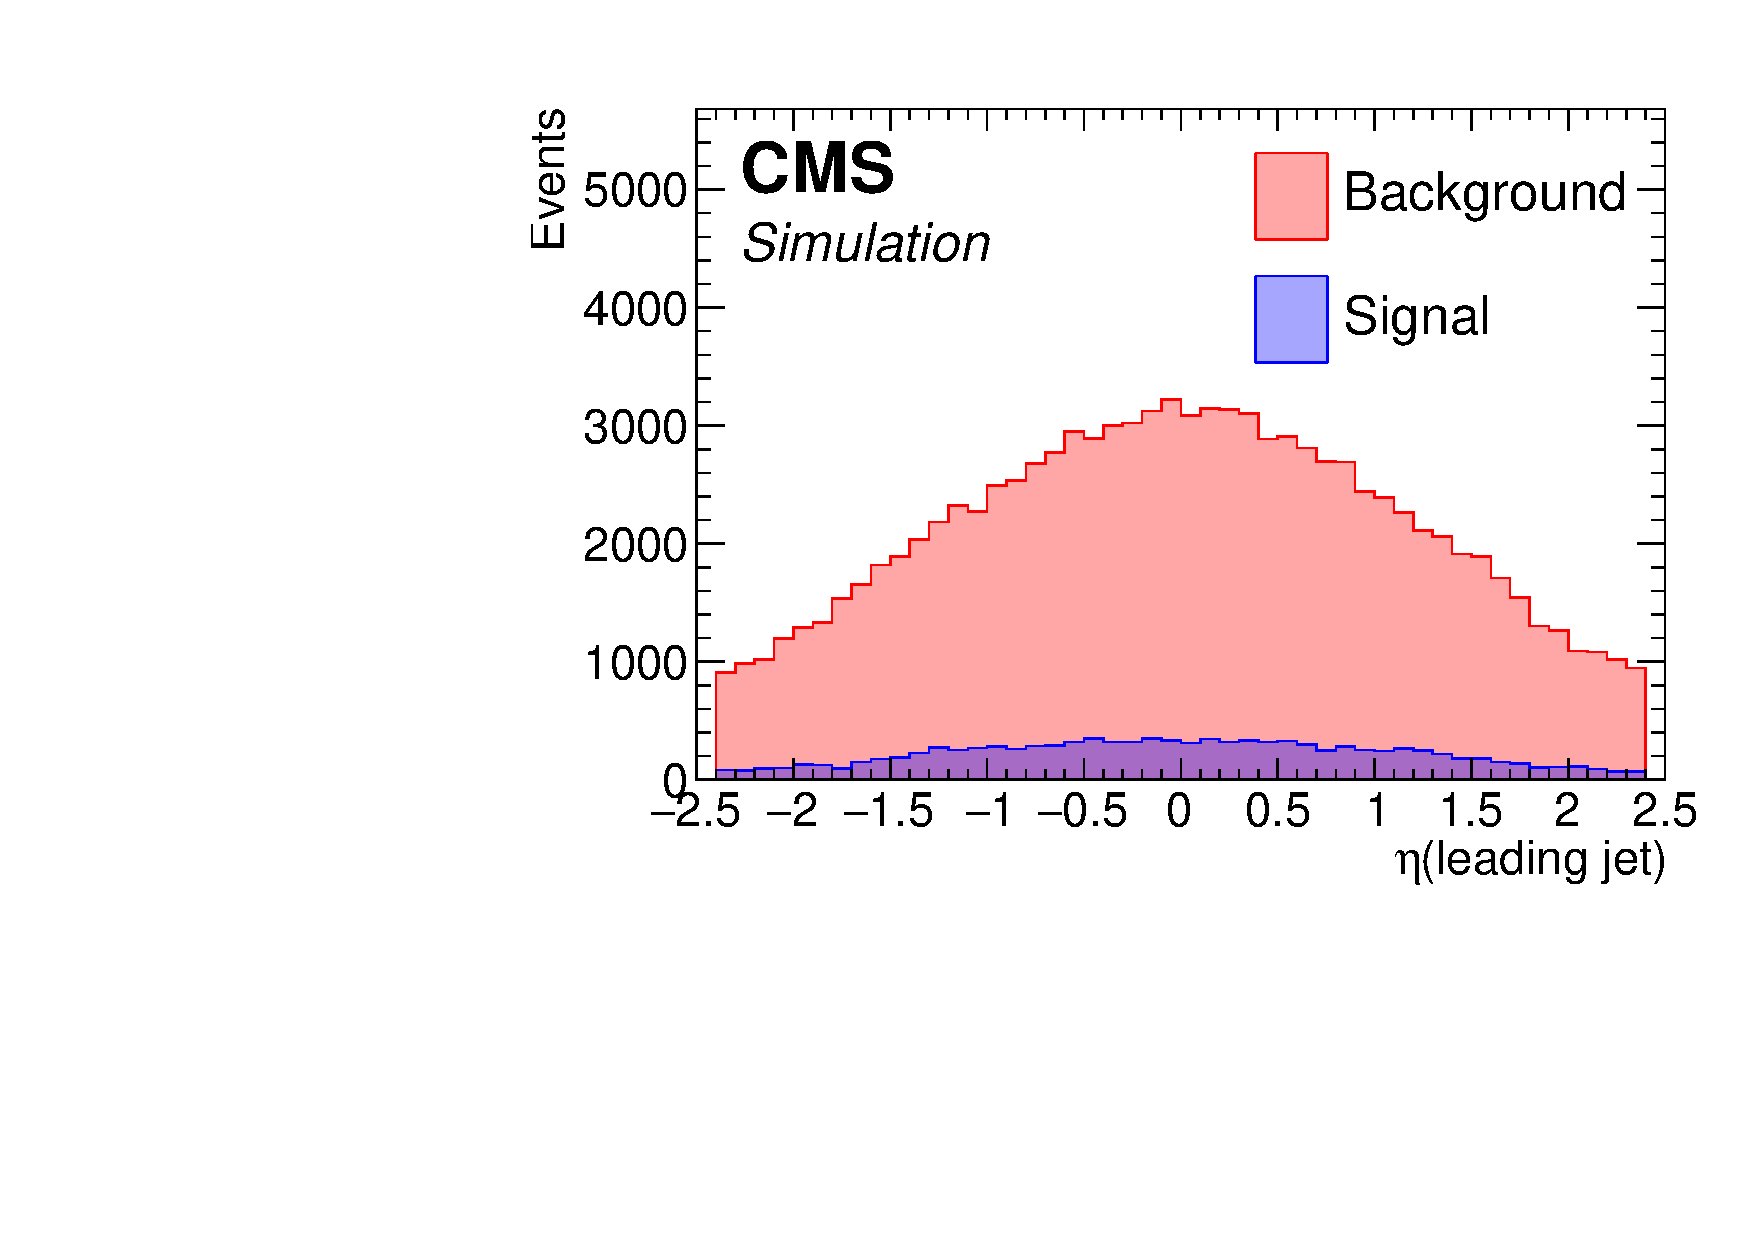
\includegraphics[width=0.32\linewidth]{plots/extrack_bdt_inputs_muons/none_LeadingJet.Eta__.pdf}   \\

\caption[exclusive track training input distribution]{Exclusive track BDT training input variables. The plots are ordered by importance ranking.}
\label{fig:extrack-input-distributions}
\end{figure}